\documentclass[10pt]{extarticle}
\title{}
\author{Avinash Iyer}
\date{}
\usepackage[shortlabels]{enumitem}

%font setup
%
%\usepackage{newpxtext,eulerpx}
\usepackage{cmbright}

%paper setup
\usepackage{geometry}
\geometry{letterpaper, portrait, margin=1in}
\usepackage{fancyhdr}

%symbols
\usepackage{amsmath}
\usepackage{amssymb}
\usepackage{mathtools}
\usepackage{hyperref}
\usepackage{gensymb}

\usepackage[T1]{fontenc}
\usepackage[utf8]{inputenc}

%chemistry stuff
\usepackage[version=4]{mhchem}
\usepackage{chemfig}

%plotting
\usepackage{pgfplots}
\usepackage{tikz}
\tikzset{middleweight/.style={pos = 0.5, fill=white}}
\tikzset{weight/.style={pos = 0.5, fill = white}}
\tikzset{lateweight/.style={pos = 0.75, fill = white}}
\tikzset{earlyweight/.style={pos = 0.25, fill=white}}
\usetikzlibrary{intersections}
\usepackage{multicol}
%\usepackage{natbib}

%graphics stuff
\usepackage{graphicx}
\graphicspath{ {./images/} }

%code stuff
%when using minted, make sure to add the -shell-escape flag
%you can use lstlisting if you don't want to use minted
%\usepackage{minted}
%\usemintedstyle{pastie}
%\newminted[javacode]{java}{frame=lines,framesep=2mm,linenos=true,fontsize=\footnotesize,tabsize=3,autogobble,}
%\newminted[cppcode]{cpp}{frame=lines,framesep=2mm,linenos=true,fontsize=\footnotesize,tabsize=3,autogobble,}

%\usepackage{listings}
%\usepackage{color}
%\definecolor{dkgreen}{rgb}{0,0.6,0}
%\definecolor{gray}{rgb}{0.5,0.5,0.5}
%\definecolor{mauve}{rgb}{0.58,0,0.82}
%
%\lstset{frame=tb,
%	language=Java,
%	aboveskip=3mm,
%	belowskip=3mm,
%	showstringspaces=false,
%	columns=flexible,
%	basicstyle={\small\ttfamily},
%	numbers=none,
%	numberstyle=\tiny\color{gray},
%	keywordstyle=\color{blue},
%	commentstyle=\color{dkgreen},
%	stringstyle=\color{mauve},
%	breaklines=true,
%	breakatwhitespace=true,
%	tabsize=3
%}
\renewcommand{\mathbf}[1]{\mathbold{#1}}
% text + color boxes
\usepackage[most]{tcolorbox}
\tcbuselibrary{breakable}
\tcbuselibrary{skins}
\newtcolorbox{problem}[1]{colback=white,enhanced,title={\small #1},
          attach boxed title to top center=
{yshift=-\tcboxedtitleheight/2},
boxed title style={size=small,colback=black!60!white},sharp corners, breakable}
%including PDFs
\setlength{\parindent}{0pt}

\pagestyle{fancy}
\fancyhf{}
\rhead{Avinash Iyer}
\lhead{Math 310: Class Notes}
\newcommand{\card}{\text{card}}
\newcommand{\ran}{\text{Ran}}
\newcommand{\N}{\mathbb{N}}
\newcommand{\Q}{\mathbb{Q}}
\newcommand{\Z}{\mathbb{Z}}
\newcommand{\R}{\mathbb{R}}
\newcommand{\F}{\mathbb{F}}
\begin{document}
  \begin{problem}{Introduction: naive set theory}
    \begin{align*}
      \mathbb{N} &= \{1,2,3,\dots,\}\\
      \mathbb{Z} &= \{0,\pm1,\pm2,\dots,\} \\
      \mathbb{Z}_+ &= \{0,1,2,\dots,\}\\
      \mathbb{Q} &= \left\{\frac{a}{b} \mid a,b\in\mathbb{Z},b\neq 0\right\}\\
      \mathbb{C} &= \{a+bi \mid a,b\in \mathbb{R}\}\\
      \mathbb{C}_q &= \{a+bi \mid a,b\in \mathbb{Q}\}
    \end{align*}
    Recall: given sets $X$ and $Y$, a relation from $X$ to $Y$ is a subset of $X\times Y$, where $\times$ denotes the cartesian product of $X$ and $Y$.\\

    A relation $f\subseteq X\times Y$ is a function from $X$ to $Y$ such that $\forall x\in X$, $\exists!y\in Y$ such that $(x,y) \in f$. We write $f(x) = y$, and denote $f$ as $f:X\rightarrow Y$.\\

    $X$ is the \textbf{domain} of $f$ and $Y$ is the \textbf{codomain}. The range $\text{Ran}(f) = \{f(x)\mid x\in X\}\subseteq Y$. \\

    The graph of a function $\text{Graph}(f) = \{(x,f(x))\mid x\in X\} \subseteq X\times Y$.
    \begin{problem}{Examples}
      \[\text{id}_x: X\rightarrow X, \text{id}_X(x) = x\]
      This is the identity function.\\

      The Characteristic Function: If $A\subseteq X$
      \[\mathbf{1}_A: X\rightarrow \mathbb{R}, ~\mathbf{1}_A(x) = \begin{cases}
        1,&x\in A\\
        0,&x\notin A
      \end{cases}\]
    \end{problem}
    \begin{problem}{Algebra of Functions}
      Let $X$ be any set, and $\mathcal(X;\mathbb{R}) = \{f:X\rightarrow \mathbb{R}\}$ represent the function space of $X$ with codomain $\mathbb{R}$.\\

      Let $f,g\in \mathcal{F}(X;\mathbb{R})$. Then, $(f+g)(x) = f(x) + g(x)$, and $(f\cdot g)(x) = f(x)\cdot g(x)$.\\

      If $t\in \mathbb{R}$, then $(tf)(x) = tf(x)$ (scalar multiplication). If $g(x)\neq 0\forall x\in X$, then $\left(\frac{f}{g}\right)(x) := \frac{f(x)}{g(x)}$.\\

      Finally, we have composition. If $f:X\rightarrow Y$ and $g:Y\rightarrow Z$ are functions, then $g\circ f(x) = g(f(x))$.
    \end{problem}
    \begin{problem}{Injective, Subjective, and Bijective}
      A function $f:X\rightarrow Y$ is a \textbf{injective} map, then, if $f(x_1) = f(x_2)$, then $x_1 = x_2$.For example, the shift map $S:\mathbb{N} \rightarrow \mathbb{N},~S(n) = n+1$ is injective.\\

      Any strictly increasing function $f:I\rightarrow \mathbb{R}$, where $I$ is any interval, is injective.\\

      A function $f$ is \textbf{surjective} if $\forall y\in Y, \exists x\in X$ such that $f(x) = y$.\\

      Consider the function $f:\mathbb{R} \rightarrow \mathbb{R},~f(x) = x^3-2x+1$. We can show that this function is surjective because $\lim_{x\rightarrow \infty}f(x) = \infty$, $\lim_{x\rightarrow -\infty} f(x) = -\infty$. Due to the intermediate value theorem, we get that $\text{ran}(f) = \mathbb{R}$.\\

      $f$ is \textbf{bijective} if it is injective and surjective.
    \end{problem}
    \begin{problem}{Invertibility}
      Let $f:X\rightarrow Y$ be a function. $f$ is \textbf{left-invertible} if $\exists g:Y\rightarrow X$ such that $g\circ f = \text{id}_X$. $f$ is \textbf{right-invertible} if $\exists h:Y\rightarrow X$ such that $f\circ h = \text{id}_Y$.\\

      $f$ is \textbf{invertible} if $\exists k:Y\rightarrow X$ such that $f\circ k = \text{id}_Y$ and $k\circ f = \text{id}_X$.\\

      For example, the function $\text{Sin}(x)$ defined as $\sin(x)$ restricted to $[-\pi/2,\pi/2]$ has an inverse, $\arcsin(x):[-1,1] \rightarrow [-\pi/2,\pi/2]$.
    \end{problem}
  \end{problem}
  \begin{problem}{Invertibility Definition}
    $f$ is invertible if and only if $f$ is left and right invertible.
    \tcblower
      Forward direction: This is via the definition of invertibility.\\

      Reverse direction: Suppose $g$ is a left-inverse of $f$, and $h$ is a right-inverse of $f$. Therefore, $g\circ f = \text{id}_X$, and $f\circ h = \text{id}_Y$. Observe that $g = g\circ \text{id}_Y$. Therefore, $g = g\circ(f\circ h)$. Via associativity, $g = (g\circ f)\circ h = \text{id}_X \circ h = h$.
  \end{problem}
  \begin{problem}{Injection and Surjection Invertibility}
    If $f:X\rightarrow Y$ is a function:
    \begin{enumerate}
      \item $f$ is injective $\Leftrightarrow$ $f$ is left-invertible.
      \item $f$ is surjective $\Leftrightarrow$ $f$ is right-invertible.
      \item $f$ is bijective $\Leftrightarrow$ $f$ is invertible.
    \end{enumerate}
    \tcblower
    We will prove the first proposition in the forward direction. Suppose $f$ is injective. Given $y\in \text{ran}(f)$, we know that $\exists! x_y\in X$ such that $f(x_y) = Y$, by the definition of injective.\\

    Let $g:Y\rightarrow X$. We will define $g$ as follows:
    \[
      g(y) = \begin{cases}
        x_y & y\in \text{ran}(f) \\
        x_0 & y\notin \text{ran}(f)
      \end{cases}
    \] 
    Where $x_0$ is an arbitrary point in $X$. We can see that $g\circ f = \text{id}_X$.
  \end{problem}
  \begin{problem}{Cardinality and Finitude}
    Which set is ``larger,'' $\{1,2,3\}$ or $\{1,2,3,4\}$? $\mathbb{N}$ or $\mathbb{N}_0$? $\mathbb{Z}$ or $\mathbb{Q}$?\\

    In order to prove that one set is ``the same size'' as the other, we can create pairs. For two sets $A$ and $B$, we can show that $A$ is the same size as $B$ by creating a function. For example, to show that $\mathbb{N}$ and $\mathbb{N}_0$ have the same size, we create $s:\mathbb{N} \rightarrow \mathbb{N}_0$, $s(n) = n+1$.

    \begin{problem}{Cardinality}
      Sets $A$ and $B$ have the same \textbf{cardinality} if $\exists$ bijection $f:A\rightarrow B$. We write $\text{card}(A) = \text{card}(B)$.
    \end{problem}
    \begin{problem}{Equivalent Cardinalities of Intervals}
      Given $a<b$ and $c<d$, we know that $\text{card}\left([a,b]\right) = \text{card}\left([c,d]\right)$.
      \tcblower
      We can create a linear function from $[a,b]$ to $[c,d]$, and since linear functions are bijections, we know that $\text{card}\left([a,b]\right) = \text{card}\left([c,d]\right)$.
    \end{problem}
    \begin{problem}{Intervals and Real Numbers}
      \[
        \text{card}\left((0,1)\right) = \text{card}(\mathbb{R})
      \] 
      \tcblower
      \begin{itemize}
        \item $\tan: (-\pi/2,\pi/2) \rightarrow \mathbb{R}$ is a bijection:
          \begin{itemize}
            \item $\tan$ is strictly increasing (and thus injective)
            \item $\lim_{x\rightarrow\infty} \tan(x) = \infty$ and $\lim_{x\rightarrow -\infty}\tan(x) = -\infty$, and by intermediate value theorem, $\tan$ is surjective
          \end{itemize}
        \item $\ell: (0,1) \rightarrow (-\pi/2,\pi/2)$ is a bijection as it is a linear function between two intervals.
        \item Therefore, our bijection is $\tan \circ \ell: (0,1) \rightarrow \mathbb{R}$.
      \end{itemize}
    \end{problem}
    \begin{problem}{Finitude}
      A set $F$ is \textbf{finite} if $F$ is empty or $\exists n\in \mathbb{N}$ such that $\text{card}(F) = \text{card}\left(\{1,2,\dots,n\}\right)$. A non-finite set is called infinite.
      \tcblower
      We can \textsl{enumerate} $F$ by creating a function $\sigma: \{1,2,\dots,n\}\rightarrow F$, such that $x_j = \sigma(j)$ for $F = \{x_1,x_2,\dots,x_n\}$.
    \end{problem}
    \begin{problem}{Inequality of Finite Sets}
      If $m\neq n$, then $\text{card}\{1,2,\dots,m\} = \text{card}\{1,2,\dots,n\}$.
      \tcblower
      WLOG, suppose $m>n$.\\

      Suppose toward contradiction that $f: \{1,2,\dots,m\} \rightarrow \{1,2,\dots,n\}$ is our bijection. This means there are $m$ ``pigeons'' and $n$ ``holes.''\\

      One hole, $j$, must contain at least two pigeons (i.e., $f(i) = f(k) = j$ for some $i\neq k\in \{1,2,\dots,m\}$). Since $f$ is assumed to be injective, this is a contradiction.
    \end{problem}
    \begin{problem}{Infinitude of the Naturals}
      $\mathbb{N}$ is infinite.
      \tcblower
      Suppose toward contradiction that $\mathbb{N}$ is finite. Thus, $\exists m\in \mathbb{N}$ such that $f:\mathbb{N} \rightarrow \{1,2,\dots,m\}$ is a bijection.\\

      Consider the inclusion $i: \{1,2,\dots,m+1\}\rightarrow \mathbb{N}$. $i$ is injective.\\

      Then, $f\circ i: \{1,2,\dots,m+1\} \rightarrow \{1,2,\dots,m\}$ is an injection, but by the pigeonhole principle, this cannot be. Therefore, we have reached a contradiction.
    \end{problem}
    \begin{problem}{Proposition}
      If $A$ is infinite, $\exists i: \mathbb{N} \xhookrightarrow{} A$.
      \tcblower
      $\exists a_1\in A$, as $A\neq \emptyset$.\\

      $A\setminus \{a_1\} \neq \emptyset$, so $\exists a_2 \in A\setminus \{a_1\}$.\\

      $A \setminus \{a_1,a_2\} \neq \emptyset$, so $\exists a_3\in A\setminus \{a_1,a_2\}$.\\

      $\vdots$\\

      We thus get a sequence $\{a_1,a_2,\dots\}$ of distinct elements of $A$.\\

      Consider $f:\mathbb{N} \rightarrow A$, $f(n) = a_n$. $f$ is injective as $a_n$ are distinct.
    \end{problem}
    \begin{problem}{Cardinality of Integers and Natural Numbers}
      \[
        \text{card}(\mathbb{Z}) = \text{card}(\mathbb{N})
      \] 
      \tcblower
      \[
        f:\mathbb{Z} \rightarrow \mathbb{N}
      \] 
      \begin{align*}
        f(m) &= \begin{cases}
          2m + 1 & m\geq 0\\
          -2m & m<0
        \end{cases}
      \end{align*}
      $f$ is a bijection as $g:\mathbb{N} \rightarrow \mathbb{Z},~g(n) = (-1)^{n+1}\left\lfloor \frac{n}{2}\right\rfloor$ is the inverse of $f$.
    \end{problem}
    \begin{problem}{Power Set}
      Given any set $X$, $\mathcal{P}(X) = \{A \mid A\subseteq X\}$ is the \textbf{power set} of $X$.\\

      $2^X:= \{f\mid f:X\rightarrow \{0,1\}\}$.
    \end{problem}
    \begin{problem}{Power Set and $2^{X}$}
      \[
        \text{card}(\mathcal{P}(X)) = \text{card}(2^X)
      \] 
      \tcblower
      Let $\varphi: \mathcal{P}(X) \rightarrow 2^X$.\\

      For $A\subseteq X$, put $\varphi(A) := \mathbf{1}_A$.\\

      Consider $\psi: 2^X \rightarrow \mathcal{P}(X)$. $\psi(f) = f^{-1}(\{1\}) = \{x\in X \mid f(x) = 1\}$.\\

      Then, $\psi\circ\varphi(A) = \psi(\mathbf{1}_A) = \mathbf{1}^{-1}(\{1\}) = A$,\\

      and, we claim $\varphi(\psi(f)) = \varphi(f^{-1}(\{1\})) = \mathbf{1}_{f^{-1}(\{1\})} = f$.
    \end{problem}
    \begin{problem}{Cantor's Theorem}
      \[
        \nexists~\text{surjection}~\mathbb{N}\rightarrow (0,1)
      \] 
      \tcblower
      Fact from calculus: $\forall \sigma\in (0,1)$, $\sigma$ can be written uniquely as a decimal expansion.
      \[
        \sigma = \sum_{k=1}^{\infty} \frac{\sigma_k}{10^k}
      \] 
      Where $\sigma_k\in \{0,1,\dots,9\}$ and not terminating in $9$s.\\

      Suppose toward contradiction that $\exists r:\mathbb{N} \rightarrow (0,1)$ that is a surjection. Write $r(n) = 0.\sigma_1(n)\sigma_2(n)\sigma_3(n)\dots$, and $\sigma_j(n) \in \{0,1,\dots,9\}$, and not terminating in $9$s.\\

      Consider $\tau: \mathbb{N} \rightarrow \{0,1,\dots,9\}$:
      \[
        \tau(n) = \begin{cases}
          3 & \sigma_n(n) = 2\\
          2 & \sigma_n(n) \neq 2
        \end{cases}
      \]
      Let $\tau = 0.\tau(1)\tau(2)\tau(3)\dots$. Since $r$ is surjective, $\exists m\in \mathbb{N}$ such that $r(m) = 0.\sigma_1(m)\sigma_2(m)\dots \sigma_m(m)\dots = \tau = 0.\tau(1)\tau(2)\dots\tau(m)\dots$.\\

      This implies that $\sigma_m(m) = \tau(m)$, which is definitionally not true, which is our contradiction.
    \end{problem}
  \end{problem}
  \begin{problem}{Comparing Cardinalities}
    \begin{itemize}
      \item $\text{card}(A) \leq \text{card}(B) \Rightarrow \exists f: A\xhookrightarrow{} B$ 
      \item $\text{card}(A) < \text{card}(B) \Rightarrow \text{card}(A) \leq \text{card}(B), \text{card}(A) \neq \text{card}(B)$
    \end{itemize}
    For example, $X\subseteq Y \Rightarrow \text{card}(X) \leq \text{card}(Y)$ because $i: X\xhookrightarrow{} Y, i(x) = x$ is an injection.\\

    \begin{problem}{Transitive Property}
      If $\text{card}(A) \leq \text{card}(B) \leq \text{card}(C)$, then $\text{card}(A) \leq \text{card}(C)$.
      \tcblower
      The composition of two injective functions is injective.
    \end{problem}
    \begin{problem}{Canonical Set Comparisons}
      Via the inclusion map, we know the following:
      \[
        \text{card}(\mathbb{N}) \leq \text{card}(\mathbb{Z}) \leq \text{card}(\mathbb{Q}) \leq \text{card}(\mathbb{R})
      \] 
    \end{problem}
    \begin{problem}{Cardinality of the Power Set}
      For any set $A$, $\text{card}(A) < \text{card}(\mathcal{P}(A))$.
      \tcblower
      Let us construct a function: $f: A \rightarrow \mathcal{P}(A)$, where $a \mapsto \{a\}$.\\

      $f$ is injective, as if $\{a\} = \{a'\}$, $a = a'$. So, $\text{card}(A) \leq \text{card}(\mathcal{P}(A))$.
      \begin{description}
        \item[Claim] $\not\exists g: A\rightarrow \mathcal{P}(A)$, $g$ is surjective.
      \end{description}
      Suppose toward contradiction that such a $g$ exists. Consider $S: \{a\in A \mid a\notin g(a)\}$.\\

      Since $g$ is onto, $\exists a_0\in A$ with $g(a_0) = S$. $a_0 \in g(a_0) \Leftrightarrow a_0\in S \Leftrightarrow a_0\notin g(a_0)$. $\bot$
    \end{problem}
    \begin{problem}{Equivalent Propositions}
      \begin{enumerate}[(i)]
        \item $\text{card}(A) \leq \text{card}(B)$
        \item $\exists f: A\xhookrightarrow{} B$
        \item $\exists g: B\rightarrow A$, $g$ surjection.
      \end{enumerate}
      \tcblower
      By definition, (i) $\Leftrightarrow$ (ii).
      \begin{description}[font=\normalfont]
        \item[(ii) $\Rightarrow$ (iii)] If $f: A\xhookrightarrow{} B$, $f$ is left-invertible, and thus $\exists g: B\rightarrow A$ with $g\circ f = id_A$. So, $g$ is right-invertible, so $g$ is surjective.
        \item[(iii) $\Rightarrow$ (ii)] If $g: B \rightarrow A$ is surjective, then $g$ is right-invertible, so $\exists f: A\rightarrow B$ such that $g\circ f = id_B$. So, $f$ is left-invertible, so $f$ is injective.
      \end{description}
    \end{problem}
    \begin{problem}{Corollary}
      If $f: A\rightarrow B$ is any map, $\text{card}(f(A)) \leq \text{card}(A)$.
      \tcblower
      Consider $g: A\rightarrow f(A)$, where $g(a) = f(a)$. So, $g$ is onto, so $\exists$ an injection $f(A) \xhookrightarrow{} A$.
    \end{problem}
    \begin{problem}{More Cardinality of Canonical Sets}
      Consider the map $q: \mathbb{Z} \times \mathbb{N} \rightarrow \mathbb{Q}, q(m,n) = \frac{m}{n}$. This map is \textsl{not} injective, as $2/4 = 1/2$. However, it is surjective, meaning $\text{card}(\mathbb{Q}) \leq \text{card}(\mathbb{Z} \times \mathbb{N})$.\\

      Earlier, we showed that $\exists h: \mathbb{Z} \leftrightarrow \mathbb{N}$. Consider $H: \mathbb{Z} \times \mathbb{N} \rightarrow \mathbb{N} \times\mathbb{N}$, defined as $H(m,n) = (h(m),n)$. 
      \begin{description}
        \item[Claim] $H$ is a bijection.
        \item[Proof of Injection] If $H(m_1,n_1) = H(m_2,n_2)$, then $h(m_1) = h(m_2)$, and $n_1 = n_2$, and since $h$ is bijective, $m_1 = m_2$, and $n_1 = n_2$, so $(m_1,n_1) = (m_2,n_2)$.
        \item[Proof of Surjection] Let $(k,\ell)\in \mathbb{N} \times \mathbb{N}$. We want to find $(m,n)\in \mathbb{Z}\times \mathbb{N}$ such that $H(m,n) = (k,\ell)$. Set $n = \ell$, and since $h$ is surjective, set $m\in \mathbb{Z}$ such that $h(m) = k$.
      \end{description}
      Therefore $\text{card}(\mathbb{Z} \times \mathbb{N}) = \text{card}(\mathbb{N}\times \mathbb{N})$.\\

      We claim that $\text{card}(\mathbb{N} \times \mathbb{N}) = \text{card}(\mathbb{N})$. First, we need to find $\varphi: \mathbb{N}\times \mathbb{N} \xhookrightarrow{} \mathbb{N}$. Consider $\varphi(m,n) = 2^m\cdot 3^n$. By the Fundamental Theorem of Arithmetic, $\varphi$ is injective.\\

      Bringing together our inequalities, we have:
      \begin{align*}
        \text{card}(\mathbb{N}) &\leq \text{card}(\mathbb{Q})\\
                                &\leq \text{card}(\mathbb{Z}\times \mathbb{N})\\
                                &=\text{card}(\mathbb{N}\times \mathbb{N})\\
                                &\leq \text{card}(\mathbb{N})
      \end{align*}
    \end{problem}
  \end{problem}
    \begin{problem}{Cardinality Rules}
      \begin{enumerate}[(i)]
        \item $\text{card}(A) \leq \text{card}(A)$ (Reflexivity)
        \item $\text{card}(A)\leq \text{card}(B) \leq \text{card}(C)\Rightarrow \text{card}(A) \leq \text{card}(C)$ (Transitivity)
        \item $\text{card}(A) \leq \text{card}(B)$ and $\text{card}(B) \leq \text{card}(A) \Rightarrow \text{card}(A) = \text{card}(B)$ (Cantor-Schröder-Bernstein)
        \item Either $\text{card}(A) \leq \text{card}(B)$ or $\text{card}(B) \leq \text{card}(A)$.
      \end{enumerate}
      \tcblower
      \begin{description}
        \item[Proof of (iii)] We have injections $f: A\xhookrightarrow{}B$ and $g:B\xhookrightarrow{} A$.\\

          Let $A_0 \setminus \text{ran}(g)$. Let $A_1 = g\circ f(A_0)$. Note that $A_0 \cap A_1 = \emptyset$. Let $A_2 = g\circ f(A_1)$. Note that $A_0\cap A_2 =\emptyset$.
          \begin{description}
            \item[Claim] We claim $A_1 \cap A_2 = \emptyset$. If $\exists z\in A_1\cap A_2$, then $z = g(f(x_0))$ for some $x_0 \in A_0$, and $z = g(f(x_1))$ where $x_1\in A_1$. However, $g$ and $f$ are injective, so $g\circ f$ is injective, so $x_0 = x_1$, but $A_0\cap A_1$. $\bot$
          \end{description}
          We let $A_n = g\circ f(A_{n-1})$ for arbitrary $n$, and $A_{\infty} = \bigcup_{n\geq 0} A_n$. If $a\notin A_{\infty}$, then $a\notin A_0$, so $a\in \text{ran}(g)$. Define $h: A\rightarrow B$.
          \[
            h(x) = \begin{cases}
              f(x) & x\in A_{\infty}\\
              y_x & x\notin A_{\infty}
            \end{cases}
          \] 
          Where $y_x$ is the unique element in $B$ with $g(y_x) = x$.
          \begin{description}
            \item[Claim] We claim $h$ is the desired bijection.
            \item[Proof of Injection] Suppose $h(x_1) = h(x_2)$.\\

              If $x_1,x_2\in A_{\infty}$, then by the definition of $H$, $f(x_1) = f(x_2)$, $f$ is injective, so $x_1 = x_2$.\\

              Suppose $x_1,x_2\notin A_{\infty}$. Then, by definition, $h(x_1) = y_{x_1}$ and $h(x_2) = y_{x_2}$, then $g(y_{x_1}) = g(y_{x_2})$, so $x_1 = x_2$.\\

              WLOG, suppose $x_1\in A_{\infty}$, and $x_2 \notin A_{\infty}$. $h(x_1) = f(x_1) = h(x_2) = y_{x_2}$. Then, $g(f(x_1))\in A_{\infty} = g(y(x_2)) = x_2\notin A_{\infty}$. This case is not possible.\\

              Thus, $h$ is injective.
            \item[Proof of Surjection] Let $y\in B$. Set $x := g(y)$.\\

              Suppose $x\notin A_{\infty}$. Then, $h(x) = y_x$, where $y_x$ is the unique element in $B$ with $g(y_x)=x=g(y)$, so $y = y_x$, so $h(x) = y$.\\

              If $x\in A_{\infty}$. We know that $x\notin A_0$, as $x\in \text{ran}(g)$. So, $x = g(f(z))$ for some $z\in A_{m-1}$. Since $g$ is injective, $y = f(z),~z\in A_{\infty}$. Thus, $h(z) = f(z) = y$.
          \end{description}
      \end{description}
    \end{problem}
  \begin{problem}{Countability}
    A set $X$ is \textsl{countable} if $\exists f: x\hookrightarrow \N$ ($\card(X) \leq\card(\N)$). $\card(\N) = \aleph_0$. If $X$ is countable and infinite, $X$ is \textit{denumerable}.
    \begin{problem}{Corollary to Cantor-Schröder-Bernstein}
      If $X$ is denumerable, then $\card(X) = \aleph_0$.
      \tcblower
      Since $X$ is infinite, $\exists f: \N\hookrightarrow X$. Since $X$ is countable, $\exists g: X\hookrightarrow \N$. By Cantor-Schröder-Bernstein, $\card(X) = \card(\N)$, so $\card(X) = \aleph_0$.
    \end{problem}
    Thus, we have: 
    \[
      \card(\N) = \card(\Z) = \card(\Q)
    \] 
    \begin{problem}{Countability under Union}
      The countable union of countable sets is countable. If $I$ is a countable indexing set and for each $i\in I$, $A_i$ is countable, then $\bigcup\limits_{i\in I} A_i$ is countable.
      \tcblower
      Since each $A_i$ is countable, $\exists \pi_i: \N \twoheadrightarrow A_i$. Consider the function
      \[
        \pi: I\times\N \rightarrow \bigcup_{i\in I}A_i
      \] 
      defined as $\pi(i,j) = \pi_i(j)$.
      \begin{description}
        \item[Claim 1] $\pi$ is a surjection.
        \item[Proof 1] Let $x\in \bigcup_{i\in I}A_i$. $\exists i_0$ such that $x\in A_{i_0}$. Since $\pi_{i_0}$ is surjective, $\exists k\in \N$ with $\pi_{i_0}(k) = x$. $\pi_{i_0}(k) = \pi(i_0,k)$. Therefore, $\pi$ is surjective.
        \item[Claim 2] $I\times\N$ is countable.
        \item[Proof 2] We know $\exists f: I\hookrightarrow\N$ since $I$ is countable. Thus, $g:I\times\N\hookrightarrow\N\times\N$, $(i,n)\mapsto (f(i),n)$. Recall, $\N\times\N\hookrightarrow \N$, $(m,n)\mapsto 2^m\cdot3^n$ is an injection. By composing these maps, $I\times\N\hookrightarrow\N$. Since $\pi$ is onto, and $I\times\N$ is countable, $\bigcup_{i\in I} A_i$ is countable.
      \end{description}
    \end{problem}
  \end{problem}
  \begin{problem}{Continuum Hypothesis}
    We saw that $\card(\N) < \card(\mathcal{P}(\N)) = \card(2^{\N})$, where $2^\N\{f\mid f:\N\rightarrow\{0,1\}\}$.
    \begin{description}
      \item[Theorem] $\card(\R) = \card(I)=\card(2^{\N})$, where $I$ is any non-degenerate interval.
    \end{description}
    \tcblower
    \begin{description}
      \item[Lemma 1] $\card([0,1]) \leq \card(2^{\N})$.
      \item[Proof 1] Every $t\in [0,1]$ has a binary expansion.
        \[
          t = \sum_{k = 1}^{\infty} \frac{\sigma_k}{2^k}
        \] 
        where $\sigma_k \in \{0,1\}$. \\

        Consider $2^{\N} \xrightarrow{\varphi} [0,1]$, defined as $\displaystyle \phi(f) = \sum_{k=1}^{\infty}\frac{f(k)}{2^k}$. Set $f: \N \rightarrow \{0,1\}$, $f(k) = \sigma_k$.\\

          Therefore, $\varphi$ is surjective, so $\exists \{0,1\}\hookrightarrow 2^{\N}$, so $\card([0,1]) \leq 2^{\N}$
        \item[Lemma 2] $\card([0,1]) = \card(\R)$.
        \item[Proof 2] We have $[0,1]\xhookrightarrow{i} \R$ via inclusion, so $\card([0,1])\leq \card(\R)$.\\

          Also, $\card(\R) = \card((0,1)) \leq \card([0,1])$, so by Cantor-Schröder-Bernstein, $\card(\R) = \card([0,1])$.
        \item[Lemma 3] Any two non-degenerate intervals $I$ and $J$ have the same cardinality. 
        \item[Proof 3] We can create injections $I\hookrightarrow J$ and vice-versa.
        \item[Lemma 4] $\card(2^{\N}) \leq \card([0,1])$.
        \item[Proof 4] $\psi: 2^{\N} \rightarrow [0,1]$. Where $\psi(f) = \sum_{k = 1}^{\infty}\frac{f(k)}{3^k}$.\\

          $\psi$ is well-defined:
          \[
            0\leq \sum_{k=1}^{\infty}\frac{f(k)}{3^k} \leq \sum_{k=1}^{\infty}\frac{1}{3^k} \leq \frac{1}{2} \leq 1
          \] 
          We claim $\psi$ is injective. Suppose $f\neq g$ in $2^{\N}$. Let $k_0 = \min\{k\mid f(k) \neq g(k)\}$. WLOG, $f(k_0) = 0, g(k_0) = 1$. Let $t_f = \sum_{k>k_0}^{\infty}\frac{f(k)}{3^k}$, $t_g = \sum_{k>k_0}^{\infty}\frac{g(k)}{3^k}$.\\

          Therefore, $\psi(f) = \sum_{k = 1}^{k_0-1}\frac{f(k)}{3^k} + 0 + t_f$, and $\psi(g) = \sum_{k=1}^{k_0-1} + \frac{1}{3^{k_0}} + t_g$.\\

          Suppose toward contradiction $\psi(f) = \psi(g)$. Then, $t_f = \frac{1}{3^{k_0}} + t_g$, or $t_f - t_g = \frac{1}{3^{k_0}}$.
          \begin{align*}
            |t_f-t_g| &= |\sum_{k>k_0}\frac{f(k)}{3^k} - \sum_{k>k_0}\frac{g(k)}{3^k}|\\
                      &\leq \sum_{k>k_0}\frac{|f(k)-g(k)|}{3^k}\\
                      &\leq \sum_{k>k_0}\frac{1}{3^{k}}\\
                      &= \frac{(1/3)^{k_0+1}}{1-(1/3)}\\
                      &= \frac{1}{2}\cdot\frac{1}{3^{k_0}}
          \end{align*}
          $\bot$
    \end{description}
    We have thus shown:
    \[
      \card(\R) = \card([0,1]) = \card(2^{\N})
    \] 
    We know that \[\aleph_0 = \card(\N) = \card(\Q) = \card(\Z) < 2^{\aleph_0} = \card(2^{\N}) = \card(\R) = \card(I)\] However, the existence of an infinity with cardinality strictly greater than $\aleph_0$ and strictly less than $2^{\aleph_0}$ is an axiom (i.e., it can be an assumption or not).
  \end{problem}
  \begin{problem}{Ordering}
    Let $X$ be a non-empty set. A relation on $X$ is a subset of $X\times X$.
    \begin{itemize}
      \item $R$ is \textsl{reflexive} if $\forall x\in X,~(x,x)\in R$.
      \item $R$ is \textsl{transitive} if $(x,y),(y,z)\in R \rightarrow (x,z)\in R$.
      \item If $R$ is \textsl{antisymmetric} $(x,y),(y,x)\in R\rightarrow x=y$. 
    \end{itemize}
    If $R$ is reflexive, transitive, and antisymmetric, then $R$ is an \textsl{ordering} of $X$.\\

    If $R$ is an ordering of $X$, then we write:
    \[
      (x,y)\in R \Leftrightarrow xRy \Leftrightarrow x\leq_{R} y
    \] 
    \begin{itemize}
      \item $x\leq_{R}x~\forall x\in X$
      \item $x\leq_R y,~y\leq_R z \rightarrow x\leq_R z$
      \item $x\leq_R y,~y\leq_R x \rightarrow x=y$
    \end{itemize}
    Additionally, $x<_R y$ means $x\leq_R y$ and $x\neq y$.
    \begin{problem}{Algebraic ordering of $\N_0$}
      $n\leq_a m\Leftrightarrow \exists k\in \N_0$ such that $n+k = m$
    \end{problem}
    \begin{problem}{$\N$ ordered via division}
      $$n\leq_D m \Leftrightarrow n|m$$
      Under this definition, it is false that $2\leq_D 5$, but it is true that $4\leq_D 20$.
    \end{problem}
    \begin{description}
      \item[Inclusion] Let $S$ be any set, and let $X = \mathcal{P}(S)$. For $A,B\in \mathcal{P}(S)$, we define $A\leq_i B \Leftrightarrow A\subseteq B$.
      \item[Containment] With $X$ defined as above, $A\leq_c B\Leftrightarrow A\supseteq B$.
    \end{description}
    For $\mathcal{F}(X,\R) = \{f\mid f:X\rightarrow\R\}$, we can define $f\leq g\Leftrightarrow f(x)\leq g(x)~\forall x\in X$.
  \end{problem}
  \begin{problem}{Types of Orderings}
    \begin{itemize}
      \item An ordering $\leq$ of $X$ is \textsl{total} or \textit{linear} if $\forall x,y\in X, x\leq y~\text{or}~y\leq x$. 
      \item An ordering is \textsl{directed} if $\forall x,y\in X~\exists z\in X$ such that $x\leq z$ and $y\leq z$.
    \end{itemize}
    If $X$ is a totally ordered set, $X$ is directed.\\

    For example, all the following orderings are directed but not total:
    \[
      (\N_0,\leq_D),~(\mathcal{P}(S),\leq_i),~(\mathcal{P}(S),\leq_c)
    \] 
  \end{problem}
  \begin{problem}{Upper/Lower Bounds}
    \begin{enumerate}[(i)]
      \item Let $(X,\leq)$ be an ordered set, $A\subseteq X$. $A$ is bounded above if $\exists v\in X$ with $a\leq v~\forall a\in A$. Such a $v$ is an upper bound.
      \item $A$ is bounded below if $\exists \ell\in X$ such that $a\geq \ell~\forall a\in A$. Such a $w$ is a lower bound.
      \item If $v$ is an upper bound of $A$ and $v\in A$, then $v$ is the greatest element of $A$, or $\max(A) = v$.
      \item If $\ell$ is a lower bound for $A$ and $\ell\in A$, then $\ell$ is the least element of $A$, or $\min(A) = \ell$.
      \item If $u$ is an upper bound for $A$, and $u \leq v$ for all other upper bounds $v$ of $A$, then $u$ is the \textsl{least upper bound} of $A$, or $\sup(A) = u$ (for \textit{supremum}).
      \item If $\ell$ is a lower bound for $A$, and $\ell \leq g$ for all other lower bounds $g$ of $A$, then $\ell$ is the \textsl{greatest lower bound} of $A$, or $\inf(A) = \ell$ (for \textit{infimum}).
      \item If $A$ is bounded above and below, then $A$ is bounded.
    \end{enumerate}
  \end{problem}
  \begin{problem}{Well-Ordering Principle}
    With $(\N,\leq_a)$, every nonempty $A\subseteq \N$ has a least element.
  \end{problem}
  \begin{problem}{Examples}
    \begin{problem}{Example 1}
      For $A\subseteq (\N,\leq_a)$, $A = \{2,3,\dots,12\}$, we have the following:
      \begin{description}
        \item[Bounded Above?] Yes.
        \item[Upper Bounds] $12,13,14,\dots$
        \item[Greatest Element] $12$
      \end{description}
    \end{problem}
    \begin{problem}{Example 2}
    For $A\subseteq (\N,\leq_D)$, $A = \{2,3,\dots,10\}$
    \begin{description}
      \item[Bounded Above?] Yes.
      \item[Upper Bounds] $10!$
      \item[Greatest Element?] No.
      \item[Supremum] $2^3\cdot3^2\cdot5\cdot7$
      \item[Bounded Below?] Yes.
      \item[Lower Bound] $1$
      \item[Least Element?] No.
      \item[Infimum] $1$
    \end{description}
    \end{problem}
    \begin{problem}{Example 3}
      For $\mathcal{A}\subseteq (\mathcal{P}(S),\leq_i)$, $A = \{A_i\}_{i\in I} \subseteq \mathcal{P}(S)$.
      \begin{description}
        \item[Supremum] $\bigcup_{i\in I}A_i$
        \item[Infimum] $\bigcap_{i\in I}A_i$
      \end{description}
    \end{problem}
  \end{problem}
  \begin{problem}{Complete Sets}
    An ordered set $(X,\leq)$ is \textsl{complete} if for all $A\subseteq X$ bounded, $\inf(A)$ and $\sup(A)$ exist.\\

    For example, $\Q$ is \textsl{not} complete, as there is not a largest rational number less than $\sqrt{2}$, for example.
  \end{problem}
  \begin{problem}{Ordering of $\Z$}
    \[
      n\leq_a m \Leftrightarrow \exists k\in \N_0,~n+k=m
    \] 
    This defines a total and complete ordering.\\

    Define $\Z^+ = \{m\in \Z\mid 0\leq_a m\}$
  \end{problem}
  \begin{problem}{Properties of $\Z^+$}
    \begin{enumerate}[(i)]
      \item $m,n\in \Z\Rightarrow m+n\in\Z^+,~m\cdot n\in \Z^+$
      \item $m\in \Z$, then $m\in \Z^+$ or $-m\in\Z^+$
      \item $m,-m\in \Z^+$, then $m=0$
      \item $m\leq_a n \Leftrightarrow n-m\in\Z^+$
    \end{enumerate}
  \end{problem}
  \begin{problem}{Ordering of $\Z$, $\Q$, and $\R$}
    Recall the ordering of $\Z$:
    \[
      n\leq_a m \xLeftrightarrow{\text{def}} \exists k\in \N_0~\text{with } n+k=m
    \] 
    \begin{description}
      \item[Claim] $\leq_a$ is an ordering of $\Z$
    \end{description}
    We claim that $\Z^+ = \{m\in\Z\mid 0\leq_a m\}$. Thus, $\Z^+ = \N_0$.
    \begin{problem}{Properties of $\Z^+$}
      \begin{enumerate}[(i)]
        \item $m,n\in \Z\Rightarrow m+n\in\Z^+,~m\cdot n\in \Z^+$
        \item $m\in \Z$, then $m\in \Z^+$ or $-m\in\Z^+$
        \item $m,-m\in \Z^+$, then $m=0$
        \item $m\leq_a n \Leftrightarrow n-m\in\Z^+$
      \end{enumerate}
    \end{problem}
    \begin{problem}{Other Properties of $\Z$}
      \begin{enumerate}[(\arabic*)]
        \item $n\leq_a m\Leftrightarrow m-n\in\Z^+$
        \item $m\leq_a n$ and $p\leq_a q$ $\Rightarrow$ $m+p \leq_a n+q$
        \item $m\leq_a n$ and $p\in \Z^+$ $\Rightarrow$ $pm\leq_a pn$
        \item $m\leq_a n$ $\Rightarrow$ $-m \prescript{}{a}\geq n$
        \item $\leq_a$ is total.
        \item If $a \prescript{}{a}>-$, and $ab \prescript{}{a}\geq 0$, then $b\prescript{}{a}>0$
        \item If $a > 0$ and $ab \prescript{}{a}\geq ac$, then $b\geq c$.
      \end{enumerate}
      \tcblower
      \begin{description}
        \item[Proof of (3):]\hfill\\
          $m\leq_a n \Rightarrow \exists k\in \N_0$ with $m+k = n$.\\
          $\Rightarrow pm + pk = pn$\\
          $pk\in \N_0$ by the properties of $\Z^+$. So, $pm \leq_a pn$
        \item[Proof of (5):]\hfill\\
          Let $m,n\in\Z$. Consider $m-n$.\\
          By (ii), $m-n\in\Z^+$ or $-(m-n)\in\Z^+$. Thus, $m-n = k$ for some $k\in\Z^+$, or $-(m-n) = \ell$ for some $\ell\in\Z^+$.\\
          Thus, $n\leq_a m$ in the first case, or $m\leq_a n$ in the second case.
      \end{description}
    \end{problem}
    We now want an ordering on $Q$.
    \begin{problem}{Creating the Rationals}
      Recall that $Q = \Z \times \Z^* = \{(a,b) \mid a\in \Z,~b\in \Z,~b\neq 0\}$. Consider the equivalence relation:
      \[
        (a,b)\sim(c,d) \xLeftrightarrow{\text{def}} ad = bc
      \] 
      We will let $\Q = \{[(a,b)]\mid (a,b) \in Q\}$ be the set of all equivalence classes in $Q$. We write:
      \[
        [(a,b)] = \frac{a}{b}
      \] 
      We define addition as follows:
      \[
        \frac{a}{b} + \frac{c}{d} = \frac{ad + bc}{bd}
      \] 
      We must check that addition is well-defined: $\frac{a'}{b'} = \frac{a}{b}$ and $\frac{c'}{d'} = \frac{c}{d}$, then $\frac{a'd' + c'b'}{b'd'} = \frac{ad+bc}{bd}$.\\

      We define multiplication as follows:
      \[
        \frac{a}{b} \cdot \frac{c}{d} = \frac{ac}{bd}
      \] 
      These operations make $\Q$ a \textbf{field}:
  \end{problem}
      \begin{problem}{Fields}
        A ring is a nonempty set set $R$ equipped with two binary operations:
        \begin{itemize}
          \item $+: R\times R \rightarrow R$, $(a,b) \mapsto a+b$ (``addition'')
          \item $\cdot: R\times R \rightarrow R$, $(a,b) \mapsto a\cdot b$ (``multiplication'')
        \end{itemize}
        such that the following hold:
        \begin{enumerate}[(1)]
          \item $(a+b)+c = a+(b+c)$
          \item $\exists z\in R$ such that $a+z = a = z+a~\forall a\in R$; there is at most one such $z$. Set $z = 0_R$.
          \item $\forall a\in R,\exists b\in R$ such that $a+b = 0_R = b+a$; there is at most one such $b$. Set $b = -a$.
          \item $\forall a,b\in R,~a+b = b+a$.
          \item $(a\cdot b)\cdot c = a\cdot(b\cdot c)$
          \item $a\cdot(b+c) = a\cdot b + a\cdot c$, $(a+b)\cdot c = a\cdot c + b\cdot c$
        \end{enumerate}
        The above six rules define a ring. If $(R,+,\cdot)$ satisfies $ab = ba$, $R$ is a commutative ring.\\

        If there exists $u\in R$ such that $ua = au = a~\forall a\in R$, $R$ is a unital ring; there is at most one unit. Set $u = 1_R$\\

        An integral domain is a unital, commutative ring such that $ab = 0 \Rightarrow a=0\vee b=0$. For example, $\Z$ is an integral domain. However, $c(\R) = \{f:\R \rightarrow \R\mid f~\text{continuous}\}$ is a unital, commutative ring, but there exist two functions such that $f,g\neq \mathbf{0}$, but $f\cdot g = \mathbf{0}$.\\

        A field is a unital, commutative ring such that every element has a multiplicative inverse.
        \[
          \forall a\in R, a\neq 0_R,\exists b\in R,~\text{with}~ab = 1_R
        \] 
        There is only one such $b$. Set $b = a^{-1}$.
      \end{problem}
      \begin{problem}{Proof that $\Q$ is a Field:}
        \[
          \left(\frac{a}{b}\right)^{-1} = \frac{b}{a}
        \] 
        Provided that $\frac{a}{b}\neq 0_{\Q}$.
      \end{problem}
      Additionally, $\Z\xhookrightarrow{j}\Q$, $j(n) = \frac{n}{1}$ is injective.
    \end{problem}
  \begin{problem}{Ordering of $\Q$}
    \[
      \frac{a}{b} \leq_a \frac{c}{d} \Leftrightarrow ad\leq_{a} bc \in \Z
    \] 
    Prove that this ordering is well-defined.

    \begin{problem}{Order Embedding}
      $\leq$ is a well-defined total ordering of $\Q$, and $j: \Z\hookrightarrow \Q$, $j(n) = \frac{n}{1}$ is an order embedding.
      \[
        j(n) \leq j(m) \Leftrightarrow n\leq_a m\in \Z
      \] 
    \end{problem}
    \begin{problem}{Properties of $\Q^+$}
      \[
        \Q^+ = \{q \in \Q \mid q \geq 0_{\Q}\}
      \] 
      \begin{enumerate}[(i)]
        \item $q_1,q_2\in \Q^+ \Rightarrow q_1 + q_2 \in \Q^+$, $q_1q_2 \in \Q^+$
        \item $q\in \Q \Rightarrow q\in \Q^+ \vee -q\in \Q^+$
        \item $\pm q\in \Q^+,q = 0$
        \item $x\leq y,!u\leq v \Rightarrow x+u \leq y+v$
        \item $x\leq y,~0\leq z \Rightarrow zx \leq zy$
      \end{enumerate}
    \end{problem}
  \end{problem}
  \begin{problem}{Ordering of $\R$, cont'd}
    An \textbf{ordered field} is a field $F$ equipped with a total ordering $\leq_{F}$ such that:
    \begin{enumerate}[(i)]
      \item if $s\leq_{F} t$, and $x\leq_{F} y$, then $s + x \leq_{F} t + y$
      \item if $s\leq_{F} t$ and $0\leq_{F} z$, then $zs\leq_{F} zt$
    \end{enumerate}
    For example, $\Q$ with its ordering is an ordered field.\\
    \begin{description}
      \item[Proposition 1:] If $(F,\leq_F)$ is an ordered field, we define $F^+ = \{x\in F,x\prescript{}{F}\geq 0\}$ with the following properties:
    \end{description}
    \begin{enumerate}[(1)]
      \item $x,y\in F^+ \Rightarrow x+y\in F^+,xy\in F^+$
      \item $x\in F \Rightarrow x\in F^+,-x\in F^+$
      \item $\pm x\in F^+ \Rightarrow x = 0_F$
    \end{enumerate}
    \begin{problem}{Proofs}
      \begin{enumerate}[(1)]
        \item Let $x,y\in F^+$. Then, $x\geq 0$  and $y\geq 0$, so by property $(i)$ of an ordered field, $x+y\geq 0+0 = 0$, so $x+y\in F^+$. Additionally, we have $x\cdot y \geq x\cdot 0 = 0$, so $xy \in F^+$.
        \item Let $x\in F$. Since the ordering on $F$ is total, $x \geq 0$ or $0\geq x$. In the first case, $x\in F^+$. In the second case, we add $-x$ to both sides, so by $(i)$, $-x\geq 0$, so $-x\in F^+$.
        \item We have $x\geq 0$  and $-x\geq 0$. So $x \geq 0$ and $x + (-x) \geq x+0$, so $x\geq 0$ and $0\geq x$. So, $x = 0$ by antisymmetry.
      \end{enumerate}
    \end{problem}
    \begin{description}
      \item[Note:] $x\leq_F y \Leftrightarrow y-x\in F^+$.
    \end{description}
    \begin{description}
      \item[Proposition 2:] Let $F$ be an ordered field. Then, the following is true:
    \end{description}
    \begin{enumerate}[(1)]
      \item $\forall a\in F$, $a^{2}\in F^+$
      \item $0,1\in F^+$
      \item If $n\in \N$, $n\cdot 1_{F} = \underbrace{1_F + 1_F + \cdots + 1_F}_{\text{$n$ times}}$
      \item If $x\in F^+$, and $x\neq 0$, then $x^{-1}\in F^+$
      \item If $xy > 0$, then $x,y\in F^+$, or $-x,-y\in F^{+}$
      \item If $0 < x \leq y$, then $0 < y^{-1} \leq x^{-1}$
      \item If $x\leq y$, then $-y\leq -x$
      \item $x\geq 1 \Rightarrow x^2 \geq x \geq 1$, and $0\leq x\leq 1 \Rightarrow 0 \leq x^2 \leq x \leq 1$.
    \end{enumerate}
    \begin{problem}{Proofs}
      \begin{enumerate}[(1)]
        \item Let $a\in F$. Then, $a\in F^+$ or $-a\in F^+$.
          \begin{description}[font=\normalfont\scshape]
            \item[Case 1] If $a\in F^+$, then by the previous proposition, $a^2\in F^+$.
            \item[Case 2] If $-a\in F^+$, then by the previous proposition, $(-a)(-a)=a^2\in F^+$.
          \end{description}
        \item $0\geq 0$, so $0\in F+$. $1 = 1\cdot 1 = 1^2 \in F^+$ by the previous result.
        \item $n\cdot 1_F = \underbrace{1_F + 1_F + \cdots 1_F}_{\text{$n$ times}}\in F^+$ by the previous proposition.
        \item Let $x\neq 0, x\in F^+$. Suppose toward contradiction that $x^{-1}\notin F^+$, then $-x^{-1}\in F^+$. Thus, $x\cdot(-x^{-1})\in F^+$, so $-1\in F^+$, but $1\in F^+$, so $1 = 0$. $\bot$
        \item Let $xy > 0$, meaning $xy\in F^+$. Suppose toward contradiction that $x>0$ and $y<0$. So, $x>0$ and $-y > 0$, so $(x)(-y) > 0$, so $-(xy) \in F^+ 0$, so $xy = 0$. $\bot$
        \item Let $0 < x \leq y$. We know $x^{-1}\in F^+$, so $x^{-1}x \leq x^{-1}y$. So $1\leq x^{-1}y$. We also know $y\in F^+$, so $y^{-1}\in F^+$. So, $1\cdot y^{-1}\leq x^{-1}\cdot y\cdot y^{-1}$. 
        \item Let $x\leq y$. Then, $0\leq y-x$, so $-y\leq -x$.
        \item Let $x\geq 1$. Then, $x\cdot x \geq 1\cdot x \geq 1$.
      \end{enumerate}
    \end{problem}
    \begin{problem}{Order Axiom}
      $\R$ is an ordered field. The injection $\Q\hookrightarrow \R$, $i(q) = q$ is an order embedding.
    \end{problem}
  \end{problem}
  \begin{problem}{Rational Orderings}
    \begin{description}
      \item[Proposition 1:] If $a\leq b$, then $a\leq \frac{1}{2}(a+b) \leq b$
    \end{description}
    \begin{problem}{Proof}
      $2a = a+a \leq a+b \leq b+b$, all by property (i) of an ordered field.\\

      Therefore, $2a \leq a+b \leq 2b$. Since $2 = 1+1 \in \R^+$, $2^{-1}\in \R^+$, so $(2a)/2 \leq \frac{1}{2}(a+b) \leq (2b)/2$, so $a\leq \frac{1}{2}(a+b) \leq b$.
    \end{problem}
    \begin{description}
      \item[Proposition 2:] If $a\geq 0$ and $(\forall \varepsilon > 0), a\leq \varepsilon$.
    \end{description}
    \begin{problem}{Proof}
      If $a\geq 0$ and $a\neq 0$, then $a > 0$. So, we have that $\frac{1}{2}a < a$. Let $\varepsilon = \frac{1}{2}a$. We also have that $a \leq \varepsilon = \frac{1}{2}a < a$, so $a<a$. $\bot$
    \end{problem}
  \end{problem}
  \begin{problem}{Arithmetic and Geometric Means}
    Given $a_1,a_2,\dots,a_n\in \R^+$:
    \begin{description}
      \item[Arithmetic Mean]
    \end{description}
    \begin{align*}
      &= \frac{\sum_{i =1}^{n} a_i}{m}
    \end{align*}
    \begin{description}
      \item[Geometric Mean]
    \end{description}
    \begin{align*}
      &= \sqrt[m]{a_1a_2\cdots a_m}
    \end{align*}
    \begin{problem}{Arithmetic Mean-Geometric Mean Inequality}
      Let $a,b \geq 0$.
      \[
        (ab)^{1/2} \leq \frac{1}{2}(a+b)
      \] 
      \tcblower
      If $x,y \geq 0$, $x\leq y \Leftrightarrow x^2 \leq y^2$.
      \begin{align*}
          0 \leq x\cdot x \leq x \cdot y \leq y\cdot y\tag*{by property (ii) of ordered fields}
      \end{align*}
      Therefore,  
      \begin{align*}
        (ab)^{1/2}&\leq \frac{1}{2}(a+b)\\
        ab &\leq \frac{1}{4}(a^2 + 2ab + b^2)\\
        4ab &\leq a^2 + 2ab + b^2 \\
        0 &\leq a^2 - 2ab + b^2\\
        0 &\leq (a-b)^2 \tag*{by definition}
      \end{align*}
      \begin{description}
        \small
        \item[Challenge:] Prove for $m$.
      \end{description}
    \end{problem}
    \begin{description}
      \item[Remark:] The harmonic mean is defined as:
    \end{description}
    \begin{align*}
      \frac{n}{\displaystyle\sum_{i=1}^{n}\frac{1}{a_i}}
    \end{align*}
  \end{problem}
  \begin{problem}{Bernoulli's Inequality}
    If $x\geq -1$, then $(1+x)^n \geq 1+nx$, for any $n\in\N_0$
    \tcblower
    By induction, we know that for $n=0$ and $n=1$, this holds.\\

    Assume the inequality holds for some $m \geq 1$.
    \begin{align*}
      (1+x)^{m+1} &= (1+x)^{m} (1+x)\\
                  &\geq (1+mx)(1+x) \tag*{by the inductive hypothesis}\\
                  &= 1+x+mx+mx^2 \\
                  &= 1+(m+1)x + mx^2\\
                  &\geq 1+(m+1)x
    \end{align*}
  \end{problem}
  \begin{problem}{Cauchy's Inequality}
    Let $a_1,\dots,a_n,b_1,\dots,b_n\in\R$. Then
    \begin{align*}
      \left|\sum_{j=1}^{n}a_jb_j\right| &\leq \left(\sum_{j=1}^{n}a_j^2\right)^{1/2}\left(\sum_{j=1}^{n}b_j^2\right)^{1/2}
    \end{align*}
    In linear algebra language, this is equivalent to $|\vec{v}\cdot\vec{w}|\leq \lVert \vec{v}\rVert \cdot \lVert\vec{w}\rVert$.
    \tcblower
    Consider $f:\R\Rightarrow \R$
    \begin{align*}
      f(x) &= \sum_{i=1}^{n}(a_j - b_jx)^2\\
      \shortintertext{We know that $f(x) \geq 0$ for all $x\in \R$}\\
           &= \sum_{i=1}^{n}(a_j^2 - 2a_jb_jx + b_j^2x^2)\\
           &= \left(\sum_{j=1}^{n}b_j^2\right)x^2 + \left(\sum_{j=1}^{n}-2a_jb_j\right)x + \sum_{j=1}^{n}a_j^2\\
           &= Ax^2 + Bx + C
      \shortintertext{Therefore, $\Delta = B^2 - 4AC \leq 0 \Rightarrow B^2 \leq 4AC$}\\
      \left(-2\sum_{j=1}^{n}a_jb_j\right)^2 &\leq 4\left(\sum_{j=1}^{n}a_j\right)\left(\sum_{j=1}^{n}b_j\right)\\
      \left|\sum_{j=1}^{n}a_jb_j\right| &= \left(\sum_{j=1}^{n}a_j\right)^{1/2}\left(\sum_{j=1}^{n}b_j\right)^{1/2}
    \end{align*}
    As we know from linear algebra, the way we get equality is when $\vec{v} = c\vec{w}$, or that $a_j = cb_j ~\forall j$ for some $c\in\R$.
  \end{problem}
  \begin{problem}{Triangle Inequality}
    Given $a_1,\dots,a_n,b_1,\dots,b_n\in\R$
    \begin{align*}
      \left(\sum_{j=1}^{n}(a_j + b_j)^2\right)^{1/2} &\leq \left(\sum_{j=1}^{n}a_j^2\right)^{1/2} + \left(\sum_{j=1}^{n}b_j^2\right)^{1/2}
    \end{align*}
    In linear algebra, this is equivalent to $\Vert\vec{v} + \vec{w}\Vert \leq \Vert\vec{v}\Vert + \Vert\vec{w}\Vert$.
    \tcblower
    \begin{align*}
      \sum (a_j + b_j)^2 &= \sum a_j^2 + \sum 2a_jb_j + \sum b_j^2\\
                         &\leq \sum a_j^2 + 2\left(\sum a_j^2\right)^{1/2}\left(\sum b_j^2\right)^{1/2} + \sum b_j^2\tag*{by Cauchy}\\
                         &= \left(\left(\sum a_j^2\right)^{1/2} + \left(\sum b_j^2\right)^{1/2} \right)^2\\
                         \shortintertext{we take square roots to get our end result}
    \end{align*}
  \end{problem}
  \begin{problem}{Metrics and Norms on $\R^n$}
    Consider $|\cdot|: \R \rightarrow \R$, defined as follows:
    \[
      |x| := \begin{cases}
        x,&x\in\R^+\\
        -x,&x\notin\R^+
      \end{cases}
    \] 
    \begin{description}
      \item[Theorems about Absolute Value:]\hfill
        \begin{enumerate}[(i)]
          \item $|ab| = |a||b|$
          \item $|a^2| = |a|^2$
          \item $|-a| = |a|$
          \item $|a|\in\R^+$
          \item $-|a| \leq a \leq |a|$
          \item $|a| \leq \delta \Rightarrow -\delta \leq a \leq \delta$ for $\delta > 0$
          \item $|a+b| \leq |a| + |b|$, $|a-b| \leq |a| + |b|$, $\vert|a| - |b|\vert \leq |a-b|$
        \end{enumerate}
    \end{description}
    \begin{problem}{Proofs}
      \begin{description}[font=\normalfont]
        \item[Proof of (i)]\hfill
          \begin{description}
            \item[Case 1:] If $a,b\in\R^+$, then $|a| = a$, and $|b| = b$, and $ab \in \R^+$, so $|ab| = ab$
            \item[Case 2:] If $a,b\notin\R^+$, then $|a| = -a$, and $|b| = -b$. Additionally, $(-a)(-b)=ab \in\R^+$, so $|ab| = ab$. The LHS $=ab$, and the RHS $=ab$.
            \item[Case 3:] $a\in\R^+$, $-b\in\R^+$. Then, $|a||b| = (a)(-b) = -ab$. Then, since $a(-b)\in\R^+$, $-ab\in\R^+$, so $|ab| = -ab$. Therefore, the LHS and RHS are equal.
          \end{description}
        \item[Proof of (vii)] Having established that $|a+b| \leq |a| + |b|$, we will show that $\vert|a| - |b|\vert \leq |a-b|$.
          \begin{align*}
            |a| &= |a-b+b| \\
                &\leq |a-b| + |b| \\
            |a| - |b| &\leq |a-b|\\
            \shortintertext{Similarly, by exchanging $a$ for $b$}\\
            |b| - |a| &\leq |b-a|\\
            |b| - |a| &\leq |a-b|\\
            \shortintertext{Let $t = |a| - |b|$. We have shown that}
            \pm t &\leq |a-b|\\
            -|a-b| \leq t &\leq |a-b|\\
            |t| &\leq |a-b|
          \end{align*}
      \end{description}
    \end{problem}
  \end{problem}
  \begin{problem}{Absolute Values, cont'd}
    Recall:
    \[
      |x| = \begin{cases}
        x,&x\in\R^+\\
        -x,&x\notin \R^+
      \end{cases}
    \] 
    If we want to find all $x\in\R$ such that $|x-1| \leq |x|$, we would split up into cases:
    \begin{description}[font=\normalfont]
      \item[$x\leq 0$] $x-1 \leq -1$, so $|x| = -x$ and $|x-1| = 1-x$, so $1-x \leq -x$, so $0 \geq 1$. $\bot$
      \item[$0 < x \leq 1$] $|x| = x$ and $|x-1| = 1-x$, so $1-x \leq x$, so $x \geq \frac{1}{2}$, so $\frac{1}{2} \leq x \leq 1$.
      \item[$1 < x$] $|x| = x$ and $|x-1| = x-1$, so $x-1 \leq x$, so $-1 \leq 0$, which is true $\forall \R$ in the interval, so $x > 1$.
    \end{description}
    Therefore, we have $x\in \left(\frac{1}{2},\infty\right)$ as that which satisfies this inequality.
  \end{problem}
  \begin{problem}{Bounded Sets}
    A subset $A\subseteq \R$ is \textbf{bounded} $\Leftrightarrow$  $\exists c \geq 0$ such that $\forall x\in A,~|x| \leq c$.
    \begin{description}
      \item[$(\Rightarrow)$] Suppose $A\subseteq \R$ is bounded. Then, $\exists \ell,u\in \R$ such that $\ell\leq x\leq u$ $\forall x\in A$. Let $c := \max\{|\ell|,|u|\}$.\\

        Since $|u| \leq c$, we have that $x\leq c$.\\

        Since $|\ell| \leq c$, and $-|\ell| \leq x$, we get that $-x \leq |\ell| \leq c$.\\

        Since $x\leq c$ and $-x\leq c$, $|x| \leq c$.
      \item[$(\Leftarrow)$] If such a $c$ exists, then $|x| \leq c$ if and only if $-c \leq x \leq c$. Thus, $-c$ is the lower bound and $c$ is the upper bound.
    \end{description}
    \begin{problem}{Bounded Functions}
      Let $D$ be any set. A function $f: D\rightarrow \R$ is bounded if $\ran(D)\subseteq \R$ is bounded.
    \end{problem}
    \begin{problem}{Example}
      Let $f: [3,7] \rightarrow \R$, $f(x) = \frac{x^2 + 2x + 1}{x-1}$. Show that $f$ is bounded.
      \tcblower
      $3\leq x \leq 7$ $\Rightarrow$ $2 \leq x-1 \leq 6$ $\Rightarrow$ $\frac{1}{6} \leq \frac{1}{x-1} \leq \frac{1}{2}$ $\Rightarrow$ $\frac{1}{|x-1|} \leq \frac{1}{2}$.\\

      Also, $4 \leq x+1 \leq 8$ $\Rightarrow$ $16 \leq x^2 + 2x + 1 \leq 64$ $\Rightarrow$ $|x^2 + 2x + 1| \leq 64$.\\

      So, $|f(x)| \leq 32$.
    \end{problem}
  \end{problem}
  \begin{problem}{Distance Metrics}
    For $s,t\in\R$, we will define $d(s,t) = |s-t|$ to be the \textbf{distance} between $s$ and $t$.

    \begin{description}
      \item[Properties:]\hfill
        \begin{enumerate}[(i)]
          \item 
          \begin{align*}
            d: &\R \times \R \rightarrow [0,\infty)\\
               &(s,t) \mapsto d(s,t) \geq 0
          \end{align*}
          \item $d(s,t) = d(t,s)$
          \item $d(s,r) \leq d(s,t) + d(t,r)$
          \item $d(s,s) = 0$
          \item If $d(s,t) = 0$, then $s = t$.
        \end{enumerate}
    \end{description}
    Let $v = \begin{pmatrix}x_1\\\vdots\\x_n\end{pmatrix}$, $ w = \begin{pmatrix}y_1\\\vdots\\y_n\end{pmatrix} \in \R^n$.
    \begin{itemize}
      \item  $1$-norm:
        \begin{align*}
          \Vert v \Vert_1 &= \sum_{j = 1}^{n} |x_j|
        \end{align*}
      \item $\infty$-norm:
        \begin{align*}
          \Vert v \Vert_{\infty} &= \max_{j=1}^{n} |x_j|
        \end{align*}
      \item $2$-norm:
        \begin{align*}
          \Vert v \Vert_2 &= \left(\sum_{j = 1}^{n} x_j^2\right)^{1/2}
        \end{align*}
    \end{itemize}
  \end{problem}
  \begin{problem}{Properties of the Norms}
    \begin{description}
      \item[Properties:] With $v,w$  above, let $p = 1,2,\infty$. The following are true:
        \begin{enumerate}[(1)]
          \item $\Vert v\Vert_p \geq 0$
          \item $\Vert v+w \Vert_p \leq \Vert v\Vert_p + \Vert w \Vert+p$
          \item $\Vert \vec{0}\Vert_p = 0$
          \item $\Vert v\Vert_p = 0 \Rightarrow v = \vec{0}$
          \item $\forall t\in \R,~\Vert tv \Vert_{p} = |t| \Vert v \Vert_p$ 
        \end{enumerate}
    \end{description}
    \begin{problem}{Proofs}
      Let $p = \infty$. We will prove (2).\\

      Say $\Vert v \Vert_{infty} = |x_i|$ and $\Vert w \Vert_{\infty} = |y_k|$. We want to show that $\Vert v + w \Vert_{\infty} = \max_{j=1}^{n}|x_j + y_j| \leq |x_i| + |y_k|$.\\

      Note that $\forall j$
      \begin{align*}
        |x_j + y_j| &\leq |x_j| + |y_j| \tag*{Triangle Inequality}\\
                    &\leq |x_i| + |y_k| \\
                    &= \Vert v \Vert_{\infty} + \Vert w \Vert_{\infty}
      \end{align*}
      Therefore, $\Vert v + w \Vert_{\infty} \leq \Vert v \Vert_{\infty} + \Vert w \Vert_{\infty}$.
    \end{problem}
  \end{problem}
  \begin{problem}{Distances and Norms}
    A \textbf{norm} on $\R^n$ is a function $\Vert \cdot \Vert: \R^n \rightarrow \R^+$, $v\mapsto \Vert v \Vert$, satisfying the following properties for $v\in\R^n$:
    \begin{enumerate}[(1)]
      \item $\Vert v \Vert \geq 0$
      \item $\Vert v + w \Vert \leq \Vert v \Vert + \Vert w \Vert$
      \item $\Vert \vec{0}\Vert = 0$
      \item $\Vert v \Vert = 0\Rightarrow v = \vec{0}$
      \item $\forall t\in\R,~\Vert tv \Vert = |t|\Vert v\Vert$
    \end{enumerate}
    If $\Vert \cdot \Vert: \R^n \rightarrow \R^+$ is a norm, we define $d_{\Vert \cdot \Vert}: \R^n \times \R^n \rightarrow \R^+$, defined as follows:
    \begin{align*}
      d_{\Vert \cdot \Vert}(v,w) = \Vert v-w \Vert
    \end{align*}
    for $v,w\in\R^n$.\\

    The properties of distance in $\R$ still hold for distance in $\R^n$:
    \begin{enumerate}[(1)]
      \item $d(v,w) = d(w,v)$
      \item $d(u,w) \leq d(u,v) + d(v,w)$
      \item $d(v,v) = 0$
      \item $d(v,w) = 0 \Rightarrow v=w$
    \end{enumerate}
  \end{problem}
  \begin{problem}{Metric Spaces}
    A \textbf{metric space} is a nonempty set $X$ equipped with a function $d: X\times X \rightarrow \R^+$, $(x,y)\mapsto d(x,y) \geq 0$. The metric has the following properties:
    \begin{enumerate}[(1)]
      \item $d(x,y) = d(y,x)$ $\forall x,y\in X$
      \item $d(x,z) \leq d(x,y) + d(y,z)$ $\forall x,y,z\in X$
      \item $d(x,x) = 0$
      \item $d(x,y) = 0 \Leftrightarrow x=y$
    \end{enumerate}
    The map $d$ is called a \textsl{metric} on $X$.
  \end{problem}
  \begin{problem}{Metric Spaces, Open Sets, and Closed Sets}
    Examples of Metric Spaces:
    \begin{itemize}
      \item $\R$ with $d(x,y) = |x-y|$.
      \item $\R^n$ with the \textsl{Euclidean metric}:
        \begin{align*}
          d_2(v,w) &= \Vert v - w \Vert_2\\
                   &= \left(\sum_{j=1}^{n}(x_j-y_j)^2\right)^{1/2}
        \end{align*}
      \item $\R^n$ with the $1$-norm:
        \begin{align*}
          d_1(v,w) &= \Vert v-w\Vert_1\\
                   &= \sum_{j=1}^{n} |x_j-y_j|
        \end{align*}
      \item $\R^n$ with the $\infty$-norm:
        \begin{align*}
          d_{\infty}(v,w) &= \Vert v-w\Vert_{\infty}\\
                          &= \max_{j=1}^{n} |x_j-y_j|
        \end{align*}
    \end{itemize}
    Let $(X,d)$ be a metric space.
    \begin{enumerate}[(1)]
      \item The \textbf{open ball} centered at $x_0\in X$ with radius $\delta$ is:
        \begin{align*}
        U(x_0,\delta) := \{x\in X \mid d(x,x_0) < \delta\}
        \end{align*}
      \item The \textbf{closed ball} centered at $x_0\in X$  with radius $\delta$ is:
        \begin{align*}
          B(x_0,\delta) := \{x\in X \mid d(x,x_0) \leq \delta\}
        \end{align*}
      \item A set $U\subseteq X$ is \textbf{open} if $\forall x\in U$, $\exists \delta > 0$ such that $U(x,\delta)\subseteq U$.
      \item A set $C\subseteq X$ is \textbf{closed} if $\overline{C} = X-C\subseteq X$ is open.
    \end{enumerate}
    \begin{problem}{Examples}
      \begin{align*}
        \shortintertext{In $\R$ with $d(s,t) = |s-t|$:}
        U(x_0,\delta) &= \{y\in\R \mid d(y,x_0) < \delta\}\\
                      &= \{y\in\R \mid |y-x_0| < \delta\}\\
                      &= (x_0-\delta,x_0+\delta)\\
        B(x_0,\delta) &= [x_0,\delta,x_0+\delta]
      \end{align*}
      The interval $A = [1,\infty)$ is not open, as $\forall \delta > 0$, $U(1,\delta)\not\subseteq [1,\infty)$.\\

      However, $A$ is closed, as $\overline{A} = (-\infty,1)$ is open: given $t\in \overline{A}$, choose $\delta = 1-t$. Let $s\in V_{\delta}(t)$. Then, $s\in (t-\delta, t+\delta)$, so $s\in (t-(1-t),t + (1-t))$, or $s\in(2t-1,1)$, so $s < 1$.
    \end{problem}
    \begin{problem}{Exercises}
      Show that the following are open:
      \begin{itemize}
        \item $(a,b)$
        \item $(a,\infty)$
        \item $(-\infty,b)$
      \end{itemize}
      and that the following are closed:
      \begin{itemize}
        \item $[a,b]$
        \item $[a,\infty)$
        \item $(-\infty,b]$
      \end{itemize}
    \end{problem}
    In $(\R^2,d_2)$, $B(0_{\R^2},1)$ is the \textbf{unit disc} centered at $(0,0)$.\\

    However, in $(\R^2,d_{\infty})$:
    \begin{align*}
      B(0_{\R^2},1) &= \{v\in\R^2 \mid \Vert v \Vert_{\infty} \leq 1\}\\
                    &= \left\{\begin{pmatrix}x\\y\end{pmatrix}\mid \max\{|x|,|y|\}\leq 1\right\}
    \end{align*}
    is the \textbf{unit square}.
  \end{problem}
  \begin{problem}{Finding a Supremum}
    Let $0\neq A\subseteq \R$. Let $u\in\R$ be an upper bound for $A$. The following are equivalent:
    \begin{enumerate}[(i)]
      \item $u=\sup(A)$
      \item If $t<u$, then $\exists a_t\in A$ such that $a_t > t$
      \item $(\forall \varepsilon > 0)(\exists a_{\varepsilon}\in A)$ with $u-\varepsilon < a_{\varepsilon}$
    \end{enumerate}
    \begin{problem}{Proofs}
      \begin{description}[font=\normalfont]
        \item[(i) $\Rightarrow$ (ii):] Given $t < u$, if no such $a\in A$ with $t < a$ exists, then $a \leq t~\forall a\in A$. Thus $t$ would be an upper bound. However, $t < u$ and $u$ is the supremum of $A$. $\bot$
        \item[(ii) $\Rightarrow$ (iii):] Given $\varepsilon > 0$, set $t = u-\varepsilon < u$. So, by (ii), $\exists a_t$ with $t < a_t$. Thus, $u-\varepsilon \leq a_t$. Set $a_{\varepsilon} = a_t$.
        \item[(iii) $\Rightarrow$ (i):] Let $v$ be an upper bound for $A$. Suppose $v < u$. Then, set $\varepsilon = u-v > 0$. By (iii), $\exists a_{\varepsilon}\in A$ with $u-\varepsilon < a_{\varepsilon}$. So $u-(u-v) < a_{\varepsilon}$, so $v < a_{\varepsilon}$, meaning $v$ cannot be an upper bound. $\bot$
      \end{description}
    \end{problem}
  \end{problem}
  \begin{problem}{Supremum Example}
    \begin{description}
      \item[$\sup [0,1) = 1$:] Certainly, $1$ is an upper bound for $[0,1)$. Let $\varepsilon > 0$.\\

        If $\varepsilon \geq 1$, pick $t = \frac{1}{2}$. Then, $1-\varepsilon < 0 < \frac{1}{2}$\\

        If $0 < \varepsilon < 1$, let $t = (1-\varepsilon) + \frac{\varepsilon}{2} = 1-\varepsilon/2$. Then, $t\in [0,1)$, and $1-\varepsilon < 1-\varepsilon/2 = t$
    \end{description}
  \end{problem}
  \begin{problem}{Finding an Infimum}
    Let $\emptyset \neq A \subseteq \R$. Let $\ell \in \R$ be a lower bound for $A$. The following are equivalent:
    \begin{enumerate}[(i)]
      \item $\ell = \inf(A)$
      \item If $t > \ell$, $\exists a_t$ such that $t > a_t$
      \item $(\forall \varepsilon > 0)(\exists a_{\varepsilon}\in A)$ with $\ell + \varepsilon > a_{\varepsilon}$
    \end{enumerate}
  \end{problem}
  \begin{problem}{Infimum Example}
    \begin{description}
      \item[$\inf\left\{\frac{1}{n}\mid n\geq 1\right\}:$] Clearly, $0 < \frac{1}{n}~\forall n \geq 1$. Let $\varepsilon > 0$.\\

        We need to find $a\in\left\{\frac{1}{n}\mid n\geq 1\right\}$ with $\varepsilon > a$. By the Archimedean Property, $\exists m\in\N$ such that $\frac{1}{m} < \varepsilon$. Let $a_{\varepsilon} = \frac{1}{m}$.
    \end{description}
  \end{problem}
  \begin{problem}{More on Supremum/Infimum}
    \begin{itemize}
      \item If $A \subseteq \R$ and $\max(A) = u$, then $u = \sup(A)$: $u$ is an upper bound of $A$ by the definition of $\max$, and if $v\neq u$ is any upper bound of $A$, then $u < v$ since $u\in A$.
      \item If $\min(A) = \ell$, then $\ell = \inf(A)$ (by the same logic).
      \item If $A$ is not bounded above, $\sup(A) = +\infty$, and if $A$ is not bounded below, then $\inf(A) = -\infty$.
      \item If $A\subseteq B$, then $\sup(A) \leq \sup(B)$.
      \item If $A\subseteq B$, then $\inf(A) \geq \inf(B)$: Let $\ell_A = \inf(A)$ and $\ell_B = \inf(B)$. By definition, $\ell_B \leq b~\forall b\in B$. Since $A\subseteq B$, $\ell_B \leq a~\forall a\in A$. Thus, $\ell_B$ is a lower bound for $A$. By definition of $\ell_A$, $\ell_B \leq \ell_A$.
    \end{itemize}
    Let $A,B\subseteq \R$ and $t\in\R$. Then, the following are also sets:
    \begin{enumerate}[(1)]
      \item $A + B = \{a+b\mid a\in A,b\in B\}$
      \item $A\cdot B = \{a\cdot b\mid a\in A,b\in B\}$
      \item $t\cdot A = \{ta\mid a\in A\}$
      \item $A + t = \{a+t\mid a\in A\}$
    \end{enumerate}
    For example, we have the following results:
    \begin{itemize}
      \item $\sup(A+B) = \sup(A) + \sup(B)$
      \item $\sup(A+t) = \sup(A) + t$
      \item $\inf(-A) = -\sup(A)$
    \end{itemize}
  \end{problem}
  \begin{problem}{Completeness Axiom}
    If $\emptyset\neq A\subseteq \R$ is bounded above, then $\sup(A)$ exists.\\

    Well-Ordering Property: if $\emptyset \neq S\subseteq \N$, then $\min(S)$ exists.\\

    Therefore, we can prove that if $F\subseteq \Z$ is bounded, then $F$ has a least and greatest element.\\

    \begin{problem}{Archimedean Property: Proof}
      If $x\in\R$, then $\exists n_x\in\N$ such that $x\leq n_x$.
      \tcblower
      Suppose there exists no natural number greater than $x$, then $\N$ is bounded above by $X$. Let $u = \sup(\N)$. By the Completeness Axiom, $u\in\R$ exists. Let $\varepsilon = 1$. Then, $\exists n\in\N$ with $u-1 < n$. So, $u < n+1$, but $n+1\in\N$, so $u$ cannot be an upper bound.
    \end{problem}
    \begin{problem}{Corollary to the Archimedean Property}
      \[
        \forall t > 0~\exists n\in\N \ni \frac{1}{n}<t
      \] 
    \end{problem}
    \begin{problem}{Corollary: Powers of 2}
      \[
        \forall t > 0~\exists m\in\N \ni \frac{1}{2^m} < t
      \] 
      \tcblower
      By the corollary to the Archimedean Property, we know that $\exists n\in \N$ such that $\frac{1}{n} < t$. By Bernoulli's inequality with $x = 1$, we have $2^n \geq n$, so $2^{-n} < n^{-1} < t$.
    \end{problem}
    \begin{problem}{Corollary: In Between Integers}
      \[
        \forall x\in\R~\exists n_x\in \Z \ni n_x-1 \leq x < n_x
      \] 
      \tcblower
      Assume $x \geq 0$. Let $S_x = \{n\mid n\in \N~x < n\}$.\\

      $S_x \neq \emptyset$ by the Archimedean Property. By the well-ordering property, let $n_x = \min(S_x)$.\\

      Therefore, $x < n_x$. Also, $n_x - 1 \notin S_x$. Therefore $n_x - 1 \leq x$.
    \end{problem}
  \end{problem}
  \begin{problem}{Density Theorems}
    Let $(X,d)$ be any metric space. A subset $D\subseteq X$ is \textbf{dense} if $\forall x\in X,~ \varepsilon > 0$, $U(x,\varepsilon) \cap D \neq \emptyset$.\\

    In the case of $X = \R$ and $d(s,t) = |s-t|$, $D\subseteq \R$ is dense if given any open interval $I$, $I\cap D \neq \emptyset$.\\

    A metric space is \textbf{separable} if it admits a \textsl{countable} dense subset.
    \begin{problem}{Density of the Rationals}
      $\Q\subseteq\R$ is dense.
      \tcblower
      Let $I = (a,b)$ be an open interval. We may assume that $a,b\in\R$ are finite.\\

      Then, $b-a > 0$. By the Archimedean property corollary, $\exists n\in\N$ such that $\frac{1}{n} < b-a$, meaning $1 < nb-na$.\\

      There exists also an integer $m$ such that $m-1 \leq na < m$, implying that $a \frac{m}{n}$. Also, $m \leq na+1 < nb$. Therefore, $\frac{m}{n} < b$.\\

      So, $\frac{m}{n}\in \Q\cap (a,b)$.
    \end{problem}
    \begin{problem}{Density of the Irrationals}
      $\R\setminus\Q$ is dense.
      \tcblower
      Assume $\sqrt{2}$ exists. Let $I = (a,b)$ be any open interval. Then, $\frac{a}{\sqrt{2}} < \frac{b}{\sqrt{2}}$.\\

      Find $q\in\Q$ such that $\frac{a}{\sqrt{2}} < q < \frac{b}{\sqrt{2}}$.\\

      Then, $a < q\sqrt{2} < b$, where $q\sqrt{2} \in\R$ and $q\sqrt{2}\notin\Q$.
    \end{problem}
    \begin{problem}{Uniqueness of $\sqrt{2}$}
      \[
        \exists! x>0~x^2 = 2
      \] 
      \tcblower
      \begin{description}[font=\normalfont]
        \item[Existence:] Let $S = \{t\in\R \mid 0 <t,~t^2<2\}$. $S$ is nonempty because $1\in\S$, and $S$ is bounded above because $y > 2 \Rightarrow y^2 > 4$.\\

          So, by the completeness axiom, $x:=\sup(S)$ exists, and $x \geq 1$.
        \item[Claim: $x^2 = 2$]
        \item[Contradiction 1:] Assume $x^2 < 2$. We want to show that $\exists n\in\N$ such that $x + \frac{1}{n}\in S$. By this assumption, we find that
          \begin{align*}
            0 < x+\frac{1}{n}\in S &\Leftrightarrow \left(x + \frac{1}{n}\right)^2 < 2\\
                                   &\Leftrightarrow x^2 + \frac{2x}{n} + \frac{1}{n^2}\\
                                   \shortintertext{Observe:}
            x^2 + \frac{2x}{n} + \frac{1}{n^2} &\leq x^2 + \frac{2x}{n} + \frac{1}{n}\\
                                               &= x^2 + \frac{1}{n}(2x+1)
                                               \shortintertext{We want to find $n\in\N$ with:}
            x^2 + \frac{1}{n}(2x + 1) < 2 &\Leftrightarrow \frac{1}{n} < \frac{2-x^2}{2x+1}
          \end{align*}
          Therefore, by the Archimedean Property corollary, we know that $n$ must exist.
        \item[Contradiction 2:] We know that $x^2\geq 2$. Since $x = \sup(S)$, $\forall m\in\N$, $\exists t_m\in S$ with $x - \frac{1}{m} < t_m$, so $\left(x-\frac{1}{m}\right)^2 < t_m^2 < 2$.\\

          Therefore, $x^2 - \frac{2x}{m} + \frac{1}{m^2}$, so $x^2 - \frac{2x}{m} < 2$, so $0 \leq x^2 - 2 < \frac{2x}{m}$.\\

          So, $0\leq \frac{x^2 - 2}{2x} < \frac{1}{m}$, so $x^2 - 2 = 0$, so $x^2 = 2$.
      \end{description}
      \begin{description}
        \item[Remark:] If we had set $S' = \{t'\in \Q\mid t^2 < 2,~t > 0\}$, we would have still obtained $\sup(S') = \sqrt{2}$. This means that $\Q$ is \textsl{not} complete.
      \end{description}
    \end{problem}
  \end{problem}
  \begin{problem}{Intervals and Nested Intervals}
    (*) Given any interval $I$, if $x_1,x_2\in I$, with $x_1 < x_2$, then $[x_1,x_2]\in I$.\\

    This seems like an obvious property, but this is the \textsl{characteristic property} of intervals.
    \begin{problem}{Characterization of Intervals}
      Let $S\in\R$ be any nonempty subset of cardinality at least $2$. Suppose $S$ satisfies (*). Then, $S$ is an interval.
      \tcblower
      \begin{description}
        \item[Case 1:] Suppose $S$ is bounded.\\

          Let $a = \inf(S)$ and $b = \sup(S)$. Then, $S \subseteq [a,b]$. We will show that $(a,b)\subseteq S$. Once this is shown, $S = \{(a,b), [a,b], [a,b), (a,b]\}$.\\

          Let $t\in (a,b)$. Since $a = \inf(S)$, $\exists x_1\in S,~x_1 \in (a,t)$. Similarly, since $b = \sup(S)$, $\exists x_2\in S,~x_1\in (t,b)$.\\

          By the hypothesis, $[x_1,x_2]\subseteq S$. Since $t\in [x_1,x_2]$, $t\in S$.
        \item[Case 2:] Suppose $S$ is bounded above, but not below.\\

          Let $b = \sup(S)$. Clearly, $S \subseteq (-\infty,b]$. We will show that $(-\infty,b)\subseteq S$. Once this is shown, $S = \{(-\infty,b), (-\infty,b]\}$.\\

          Let $t\in (-\infty,b)$. Since $b = \sup(S)$, $\exists x_2\in S,~x_2\in (t,b)$.\\

          Since $S$ is not bounded below, $\exists x_1\in S$ such that $x_1 < t$ (or else $t$ would be a lower bound).\\

          By the hypothesis, $[x_1,x_2]\in S$, and $t\in [x_1,x_2]$, so $t\in S$.
        \item[Case 3, 4:] Left as an exercise for the reader.
      \end{description}
    \end{problem}
    A sequence of intervals $(I_n)_{n \geq 1}$ is called \textsl{nested} if
    \begin{align*}
      I_1 \supseteq I_2 \supseteq \dots I_n \supseteq I_{n+1} \supseteq\dots
    \end{align*}
    We are primarily interested in $\bigcap I_n$.
    \begin{enumerate}[(a)]
      \item $\bigcap_{n=1}[0,1/n) = \{0\}$.
      \item $\bigcap_{n=1}(0,1/n) = \emptyset$
      \item $\bigcap_{n=1}[n,\infty) = \emptyset$
    \end{enumerate}
  \end{problem}
  \begin{problem}{Measure}
    The \textbf{measure} of an interval is basically its ``size.''
    \begin{enumerate}[(a)]
      \item $m([a,b]) = b-a$
      \item $m((a,b]) = b-a$
      \item $m((a,b)) = b-a$
      \item $m([a,b)) = b-a$
    \end{enumerate}
  \end{problem}
  \begin{problem}{Nested Intervals Theorem}
    Let $I_n = [a_n,b_n]$ for $n\in\N$ be a nested sequence of intervals.
    \begin{enumerate}[(1)]
      \item $\bigcap_{n \geq 1}I_n \neq \emptyset$
      \item If $\inf\left\{m(I_n)\mid n\geq 1\right\} = 0$, then $\bigcap_{n\geq 1} I_n = \{\xi\}$
    \end{enumerate}
    \tcblower
    \begin{problem}{(a)}
      Since $[a_1,b_1] \supseteq [a_2,b_2] \supseteq \dots$, we have that $a_1\leq a_2\leq a_3,\dots$, and $b_1 \geq b_2 \geq b_3 \geq \cdots$.\\

      We know that $\{a_n\}$ is bounded above and nonempty. Let $\xi = \sup\left(\left\{a_n\right\}_{n=1}^{\infty}\right)$.\\

      We know that $\{b_n\}$ is bounded below. Let $\eta = \inf\left(\left\{b_n\right\}_{n=1}^{\infty}\right)$.\\

      We claim that $\xi \leq b_n$ $\forall n \geq 1$. Suppose toward contradiction that $\exists m$ such that $\xi > b_m$. Then, by the supremum property, $\exists a_i$ such that $\xi > a_i > b_m$. If $k\leq m$, $a_k \leq a_m \leq b_m < a_k$. If $m \leq k$, then $b_m \geq b_k \geq a_k > b_m$. $\bot$\\

      Similarly, using the same argument, $a_n \leq \eta~\forall n$.\\

      Thus, $\xi \leq \eta$.\\

      We claim that $\bigcap_{n\geq 1} I_n = [\xi,\eta]$. If $t\in [\xi,\eta]$, then $a_n \leq \xi \leq t \leq \eta \leq b_n$. So $t\in [a_n,b_n]~\forall n$, so $t\in \bigcap_{n\geq 1} [a_n,b_n]$.\\

      If $t\in \bigcap_{n\geq 1}I_n$, then $t\in [a_n,b_n]~\forall n$, so $a_n \leq t \leq b_n$ $\forall n$. So, $t$ is an upper bound on $a_n$, and a lower bound on $b_n$. So, $\xi \leq t \leq \eta$ by definition of $\xi$ and $\eta$.
    \end{problem}
    \begin{problem}{(b)}
      We have $\forall n\geq 1$
      \begin{align*}
        [\xi,\eta] &\subseteq [a_n,b_n]\\
        \Rightarrow 0 \leq \eta-\xi &\leq b_n-a_n\\
                                    &= m(I_n)
      \end{align*}
      So, if $\inf\left(\{m(I_n)\mid n\geq 1\right) = 0$, then $0\leq \eta-\xi \leq 0$, so $\eta = \xi$.
    \end{problem}
  \end{problem}
  \begin{problem}{Corollary to the Nested Intervals Theorem}
    $[0,1]$ is uncountable.
    \tcblower
    Suppose it is possible to denumerate the interval $[0,1] = \{t_1,t_2,\dots,\}$.\\

    We can find $[a_1,b_1]\subseteq [0,1]$ with:
    \begin{itemize}
      \item $a_1 < b_1$
      \item $t_1\notin [a_1,b_1]$.
    \end{itemize}
    Then, we find $[a_2,b_2]\in [a_1,b_1]$ with $a_2 < b_2$, $t_2\notin [a_2,b_2]$.\\

    Recursively, we find $[a_n,b_n]\subseteq [a_{n-1},b_{n-1}]$ with $a_n < b_n$, $t_n\notin [a_n,b_n]$.\\

    So, $I_n = ([a_n,b_n])_{0}^{\infty}$ is a sequence of nested intervals.\\

    Therefore, $\exists \xi\in \bigcap I_n \subseteq [0,1]$. However, $\xi \notin \{t_1,t_2,\dots\}$. $\bot$
  \end{problem}
  \begin{problem}{Sequences in Metric Spaces}
    A sequence in a metric space $M$ is a map
    \begin{align*}
      x&: \N \rightarrow M \tag*{$M = \R$, usually}\\
      x &= \left(x_n\right)_{n=1}^{\infty}
    \end{align*}
    \begin{description}
      \item[I.] Sequences defined by a formula:
        \begin{enumerate}[(i)]
          \item $x_n = t$ (the constant sequence)
          \item $x_n = 2n + 1$
          \item $x_n = \frac{1}{n-1}$ (here, $n \geq 2$)
          \item $c_n = n\sin\left(\frac{1}{n}\right)$
          \item $d_n = \left(1 + \frac{1}{n}\right)^n$
          \item Geometric \textsl{Sequence}: for $b\neq 0$, $(b^n)_{n\geq 0} = (1,b,b^2,\dots)$
          \item $x_n = \frac{n!}{n^n}$
          \item Given any function
            \begin{align*}
              f:[0,\infty)\rightarrow\R
            \end{align*}
            we can set $x_n = f(n)$.
        \end{enumerate}
      \item[II.] Sequences defined recursively:
        \begin{enumerate}[(i)]
          \item $a_1 = 1,~a_{n+1}=2a_n + 1 = (1,3,7,15,\dots)$
          \item Fibonacci: $f_1 = 1,~f_2 = 1,~f_{n+1} = f_{n} + f_{n-1} = (1,1,2,3,5,8,\dots)$. The closed form equation is:
            \begin{align*}
              f_n = \frac{1}{\sqrt{5}}\left(\varphi^n - (1-\varphi)^n\right)
            \end{align*}
            where $\varphi = \frac{1 + \sqrt{5}}{2}$
          \item Let $f: M\rightarrow M$ be a self-map on a metric space. Fix $x_0\in M$.\\

            \[x_n = \underbrace{f\circ f\cdots \circ f}_{n~\text{times}}(x_0)\]
        \end{enumerate}
      \item[III.] New sequences from old: 
        \begin{enumerate}[(i)]
          \item Let $(a_n)_n$ and $(b_n)_n$ be sequences, $t\in\R$. Then, we can do the following:
            \begin{itemize}
              \item $(a_n)_n + (b_n)_n + (a_n + b_n)_n$
              \item $t(a_n)_n = (ta_n)_n$
              \item $(a_n)_n(b_n)_n = (a_nb_n)_n$
              \item If $b_n \neq 0~\forall n, \left(\frac{a_n}{b_n}\right)$
            \end{itemize}
          \item We can also shift a sequence:
            \begin{align*}
              x_{n+1} = (x_2,x_3,\dots)
            \end{align*}
          \item We can look at ratios for $a_n\neq 0$
            \begin{align*}
              r_n = \frac{a_{n+1}}{a_n}
            \end{align*}
          \item We can look at partial sums, given $(a_k)_{k=1}^{\infty}$.
            \begin{align*}
              s_1 &= a_1\\
              s_n &= s_{n-1} + a_n\\
                  &= \sum_{k=1}^{n}a_k
            \end{align*}
            The sequence $(s_n)_n$ is called the sequence of partial sums. For example, the sequence of partial sums for $(b^k)_{k=0}^{\infty}$ is:
            \begin{align*}
              1 + b + b^2 + \cdots + b^n = \begin{cases}
                \frac{1-b^{n+1}}{1-b}&b\neq 1\\
                n+1&b=1
              \end{cases}
            \end{align*}
            because for $b \neq 1$, $(1-b)(1+b+b^2+\cdots+b^n) = 1-b^{n+1}$
        \end{enumerate}
    \end{description}
    \begin{problem}{Exercise}
      Let $a_k = \frac{1}{k(k+1)}$. Find $(s_n)_n$.
      \tcblower
      Via partial fraction decomposition, we get that $\frac{1}{k(k+1)} = \frac{1}{k}-\frac{1}{k+1}$. Therefore, $(s_n)_n = \left(1-\frac{1}{n+1}\right)_{n=1}^{\infty}$
    \end{problem}
  \end{problem}
  \begin{problem}{Bounded Sequences}
    \[
      \ell_{\infty} = \left\{(a_k)_k \mid a_k\in\R,~a_k~\text{bounded}\right\}
    \] 
    We define
    \begin{align*}
      \Vert(a_k)_k\Vert_{\infty} = \sup_{k\geq 1}|a_k|\tag*{Infinity Norm}
    \end{align*}
    This norm has the traditional properties of the norm:
    \begin{align*}
      \Vert (a_k)_k + (b_k)_k\Vert_{\infty} &\leq \Vert(a_k)_k\Vert_{\infty} + \Vert(b_k)_k\Vert_{\infty}\tag*{Triangle Inequality}\\
      \Vert t(a_k)_k\Vert_{\infty} &= |t|\Vert(a_k)_k\Vert_{\infty}\tag*{Scalar Multiplication}\\
      \Vert(a_k)_k\Vert_{\infty} = 0 &\Leftrightarrow a_k = 0~\forall k\tag*{Zero Property}\\
      \Vert(a_k)_k(b_k)_k\Vert_{\infty} &\leq \Vert(a_k)_k\Vert_{\infty}\Vert(b_k)_k\Vert_{\infty}\tag*{Multiplication}
    \end{align*}
    \begin{problem}{Proof}
      Let $u = \Vert(a_k)_k\Vert_{\infty}$ and $v = \Vert(b_k)_k\Vert_{\infty}$.\\

      Given any $k$,
      \begin{align*}
        |a_k + b_k| &\leq |a_k| + |b_k| \tag*{Triangle Inequality on $|\cdot|$}\\
                    &\leq u+v \tag*{definition of supremum}\\
        \Rightarrow \sup_{k\geq 1}|a_k + b_k|&\leq u+v
      \end{align*}
      Thus,
      \begin{align*}
        \Vert (a_k)_k + (b_k)_k\Vert_{\infty} &= \Vert \left((a_k + b_k)_k\right)_k\Vert_{\infty}\\
                                              &= \sup_{k\geq 1}|a_k + b_k|\\
                                              &\leq u+v
      \end{align*}
    \end{problem}
  \end{problem}
  \begin{problem}{Monotonicity}
    A sequence $(x_n)_n$ is \textbf{increasing} if
    \begin{align*}
      x_1 \leq x_2 \leq \cdots~\forall n
    \end{align*}
    and is \textbf{decreasing} if
    \begin{align*}
      x_1 \geq x_2 \geq \cdots~\forall n
    \end{align*}
    The sequence is \textsl{eventually} increasing if $\exists m\in \N \ni x_n \leq x_{n+1}$ for $n > m$.\\

    Similarly, the sequence is eventually decreasing if $\exists m\in\N \ni x_n \geq x_{n+1}$ for $n > m$.\\

    A sequence that is increasing or decreasing is \textbf{monotone} (or eventually monotone).\\

  \end{problem}
  \begin{problem}{Monotonicity Example}
    The sequence
    \begin{align*}
      a_1 &= 1\\
      a_{n+1} &= \frac{1}{2}a_n + 2
    \end{align*}
    is increasing and bounded above.
    \tcblower
    We will prove the first statement via induction:
    \begin{description}
      \item[Base:] $a_1 = 1$, $a_2 = \frac{1}{2} + 2 = \frac{5}{2} \geq 1$
      \item[Inductive Hypothesis] $a_n \leq a_{n+1} \Rightarrow a_{n+1} \leq a_{n+1}$
      \item[Proof:]
        \begin{align*}
          a_{n} &\leq a_{n+1}\\
          \frac{1}{2}a_n &\leq \frac{1}{2}a_{n+1}\\
          \frac{1}{2}a_n + 2 &\leq \frac{1}{2}a_{n+1} + 2\\
          a_{n+1} &\leq a_{n+2}
        \end{align*}
    \end{description}
    To prove the sequence is bounded above, we do the following:
    \begin{align*}
      a_1 = 1 &\leq 4\\
      \frac{1}{2}a_1 &\leq 2\\
      \frac{1}{2}a_1 + 2 &\leq 2\\
      a_{2} &\leq 4
    \end{align*}
    We claim that $\forall n,~a_n \leq 4 \Rightarrow a_{n+1} \leq 4$, as we have shown the base case.
    \begin{align*}
      a_{n} &\leq 4\\
      \frac{1}{2}a_n &\leq 2\\
      \frac{1}{2}a_n + 2 &\leq 4\\
      a_{n+1} &\leq 4
    \end{align*}
  \end{problem}
  \begin{problem}{Convergence of Sequences}
    Let $L\in\R$, $\varepsilon > 0$. Then, the $\varepsilon$\textbf{-neighborhood} of $L$ is $(L-\varepsilon, L+\varepsilon) = V_{\varepsilon}(L)$.
    \begin{align*}
      x\in V_{\varepsilon}(L)\\
      \Leftrightarrow\\
      |x-L| < \varepsilon\\
      L-\varepsilon < x < L+\varepsilon
    \end{align*}
    With this in mind, we know the following:
    \begin{problem}{Definition of Convergence}
      A real sequence $(x_n)_n$ converges to a number $x$ if 
      \begin{align*}
        \left(\forall \varepsilon > 0\right)\left(\exists N_{\varepsilon}\in\N\right) \ni n\geq N \Rightarrow |x_n-x| < \varepsilon
      \end{align*}
      If no such $L$ exists, then $(x_n)_n$ is said to \textbf{diverge}.\\

      A sequence $(x_n)_n$ in a metric space $(X,d)$ converges to a point $x$ if
      \begin{align*}
        \left(\forall \varepsilon > 0\right)\left(\exists N_{\varepsilon}\in\N\right) \ni d(x_n,x) < \varepsilon
      \end{align*}
    \end{problem}
    Essentially, we want to show that there always exists an $N$ such that the $N$th tail (i.e., $x_{N}, x_{N+1},\cdots$) are within $\varepsilon$ of $L$ for any $\varepsilon$.
    \begin{description}
      \small
      \item[Note:] $N$ usually depends on $\varepsilon$ (the smaller the $\varepsilon$, the larger the $N$).
    \end{description}
    \begin{problem}{Convergence Proof}
      \begin{align*}
        \left(\frac{1}{n}\right)_{n} \xrightarrow{n\rightarrow\infty} 0
      \end{align*}
      \tcblower
      We know that
      \begin{align*}
        |x_n - L| &= \left|\frac{1}{n}\right|
      \end{align*}
      Given $\varepsilon > 0$, we want $\frac{1}{n} < \varepsilon$, meaning $n > \frac{1}{\varepsilon}$.
      \begin{description}
        \item[Proof:] Let $\varepsilon > 0$. By the Archimedean property corollary, find $N\in\N$ large such that $\frac{1}{N} < \varepsilon$.
          \begin{align*}
            n &\geq N\\
            \frac{1}{n} &\leq \frac{1}{N}\\
                        &< \varepsilon\\
            \shortintertext{so, if $n\geq N$, then}
            |x_n - L| &= \left|\frac{1}{n}\right|\\
                      &= \frac{1}{n}\\
                      &< \varepsilon
          \end{align*}
      \end{description}
    \end{problem}
    \begin{problem}{Convergence Proof 2}
      Show that
      \begin{align*}
        \left(\frac{5n-1}{3-n}\right)_{n\geq 4} \xrightarrow{n\rightarrow\infty} -5
      \end{align*}
      \tcblower
      \begin{align*}
        |x_n - L| &= \left|\frac{5n-1}{3-n} + 5\right|\\
                  &= \frac{14}{|3-n|}\\
                  &= \frac{14}{n-3}
                  &< \varepsilon\\
        \frac{14}{n-3} &< \varepsilon\\
        n > \frac{14}{\varepsilon} + 3
      \end{align*}
      \begin{description}
        \item[Proof:] Let $\varepsilon > 0$. Find $N' \in\N$ so large that $\frac{1}{N'} < \frac{\varepsilon}{14}$ (which exists by the Archimedean property corollary). Let $N = N' + 3$. If $n \geq N$, then
          \begin{align*}
            n-3 &\geq \frac{1}{N'}\\
            \frac{1}{n-3} &\leq \frac{1}{N'}\\
                          &< \frac{\varepsilon}{14}\\
                          \shortintertext{whence}
            |x_n - L| &= \frac{14}{n-3}\\
                      &< \frac{14\varepsilon}{14}\\
                      &= \varepsilon
          \end{align*}
      \end{description}
    \end{problem}
  \end{problem}
  \begin{problem}{Sequences and their Limits, cont'd}
    \begin{problem}{Convergence and Distance}
      Let $(X,d)$ be a metric space, and let $(x_n)_n$ be a sequence in the metric space. The following are equivalent:
      \begin{enumerate}[(i)]
        \item $(x_n)_n\rightarrow x$
        \item $\left(d(x_n,x)\right)_n \rightarrow 0$
      \end{enumerate}
      \tcblower
      \begin{description}[font=\normalfont]
        \item[(i) $\Rightarrow$ (b)] Let $\varepsilon > 0$. Find $N_{\varepsilon}\in\N$ so large such that $d(x_n,x) < \varepsilon$ whenever $n \geq N_{\varepsilon}$.\\

          So, $|d(x_n,x)-0| = d(x_n,x) < \varepsilon$ for all $\varepsilon > 0$. Whence, $\left(d(x_n,x)\right)_n \rightarrow 0$.
        \item[(ii) $\Rightarrow$ (i)] This direction is similar.
      \end{description}
    \end{problem}
    In $\R$, this implies that
    \begin{align*}
      (x_n)_n \rightarrow x\\
      \Leftrightarrow\\
      (|x_n -x|)_n \rightarrow 0
    \end{align*}
    \begin{problem}{Comparison Proposition}
      Let $(X,d)$ be a metric space and let $x\in X$, and suppose $(x_n)_n$ is a sequence in $X$.\\

      If $\exists c\geq 0$, $m\in\N$, and a sequence $(a_n)_n\in\R^+$ with $(a_n)_n \rightarrow 0$ and $d(x_n,x) \leq c a_n~\forall n > m$. Then, $(x_n)_n\rightarrow x$.
      \tcblower
      Let $\varepsilon > 0$. Note that $\frac{\varepsilon}{c} > 0$.\\

      Find $N_1\in \N$ large such that $n \geq N_1 \Rightarrow |a_n - 0| < \frac{\varepsilon}{c}$, which is always possible since $(a_n)_n \rightarrow 0$.\\

      Let $N = \max(N_1,m)$. Then, $n \geq N\Rightarrow n\geq N_1$ and $n\geq m$. So,
      \begin{align*}
        d(x_n,x) &\leq ca_n\\
        &< c\frac{\varepsilon}{c}\\
        &=\varepsilon
      \end{align*}
      so, $n\geq N \Rightarrow d(x_n,x) < \varepsilon$, whence $(x_n)_n \rightarrow x$
    \end{problem}
    \begin{problem}{Comparison Proposition, Example 1}
      Prove
      \begin{align*}
        \left(\frac{\sin(n^2-1)}{n^2 + 3}\right)_n \rightarrow 0
      \end{align*}
      \tcblower
      \begin{align*}
        \left|\frac{\sin(n^2 - 1)}{n^2 + 3} - 0\right| &= \frac{|\sin(n^2 - 1)|}{n^2 + 3}\\
                                                       &\leq \frac{1}{n^2 + 3}\\
                                                       &\leq \frac{1}{n^2}\\
                                                       &\leq \frac{1}{n}
      \end{align*}
      We know that $a_n = \frac{1}{n}$ converges to $0$. So, by our comparison proposition, we are done.
    \end{problem}
    \begin{problem}{Comparison Proposition, Example 2}
      Prove
      \begin{align*}
        \left(\frac{1}{2^n}\right)_n \rightarrow 0
      \end{align*}
      \tcblower
      \begin{align*}
        2^n &= (1+1)^n\\
            &\geq 1+n\tag*{Bernoulli's Inequality}\\
            &>n\\
            \shortintertext{so,}
        \frac{1}{2^n} &< \frac{1}{n}
      \end{align*}
      Since $a_n = \frac{1}{n}$ converges, we know that $\frac{1}{2^n}$ must converge.
    \end{problem}
  \end{problem}
  \begin{problem}{Sequence Divergence}
    A sequence $(x_n)_n$ is \textbf{divergent} if it does not converge. $(x_n)_n \rightarrow 0$ if and only if
    \begin{align*}
      (\forall \varepsilon > 0)(\exists N_{\varepsilon} \in \N) \ni (\forall n\geq N_{\varepsilon}) d(x_n,x) < \varepsilon
    \end{align*}
    So, $(x_n)_n$ diverges if and only if
    \begin{align*}
      (\exists \varepsilon_0 > 0)(\forall N\in\N) (\exists n\geq N) \rightarrow d(x_n,x)\geq \varepsilon_0
    \end{align*}
    \begin{problem}{Diverging Sequence Proof}
      Show that the following sequence diverges:
      \begin{align*}
        a_n &= (-1)^n
      \end{align*}
      \tcblower
      \begin{description}
        \item[Step 1]
          \begin{align*}
            \left((-1)^n\right)_n \not\rightarrow 1
          \end{align*}
          Take $\varepsilon_0 = 1/2$, given any $N\in\N$, we will find $n\geq N$ odd:
          \begin{align*}
            n &= 2N+1\\
            d((-1)^n,1) &= 2\\
                        &\geq \varepsilon_0
          \end{align*}
        \item[Step 2]
          \begin{align*}
            \left((-1)^n\right)_n \not\rightarrow -1
          \end{align*}
          by letting $\varepsilon_0 = 1/2$ and $n = 2N$.
      \end{description}
    \end{problem}
    \begin{problem}{Diverging Sequence Proof 2}
      Does
      \begin{align*}
        a_n &= \left(\sin(n)\right)_n
      \end{align*}
      converge?
      \tcblower
      It is not the case that $\left(\sin(n)\right)_n \rightarrow L$ for any $L\in\R$.
      \begin{description}
        \item[Case 1] If $L > 1$, set $\varepsilon_0 = \frac{L-1}{2}$. Then, given any $N\in\N$, pick $n = N$.
          \begin{align*}
            |\sin(n)-L| &= L-\sin(n)\\
                        &\geq L-1\\
                        &> \frac{L-1}{2}\\
                        &= \varepsilon_0
          \end{align*}
        \item[Case 2] Similarly for $L < -1$
        \item[Case 3] Suppose $-1 < L < 1$.
          \begin{description}
            \item[Case 3.1] Suppose $L > 0$. Set $\varepsilon_0 = \frac{L}{2}$. Given any $N$, find $n \geq N$ with $\sin(n) < 0$. \\

              We find $k$ large such that $N < (2k+1)\pi$, which we can always do because we are finding $k > \frac{1}{2}\left(\frac{N}{\pi} - 1\right)$, which is always possible by the Archimedean property.\\

              Note that $N < (2k+1)\pi < (2k+2)\pi$. Note that $\sin(x) < 0$ on the interval $((2k+1)\pi,(2k+2)\pi)$. Note that $|(2k+1)\pi - (2k+2)\pi| = \pi$. Let $n = \lceil (2k+1)\pi\rceil$. Then, $|L-\sin(n)| \geq \frac{L}{2} = \varepsilon_0$
            \item[Case 3.2] Suppose $L < 0$, set $\varepsilon_0 = \frac{-L}{2}$. Given $N$, find $n \geq N$ with $\sin(n) > 0$. Using the same strategy as above, we find $n$ such that $|L - \sin(n)| > \varepsilon_0$
            \item[Case 3.3] Suppose $L = 0$. Set $\varepsilon_0 = 1/2$. Given $N\in\N$, find $n\geq N$ with $\sin(n) \geq \frac{1}{2}$. Then, $|\sin(n)-0| = \sin(n) \geq \varepsilon_0$.
          \end{description}
      \end{description}
    \end{problem}
    Showing that a sequence diverges is not easy --- later, we will divergence with non-uniqueness of convergent subsequences.
  \end{problem}
  \begin{problem}{Alternating Series}
    Consider again
    \begin{align*}
      \left((-1)^n\right)_{n\geq 0} &= (1,-1,1,-1,\dots)
    \end{align*}
    The even entries converge to $1$:
    \begin{align*}
      \left((-1)^n\right)_{2n} &= (1,1,1,\dots)
    \end{align*}
    Similarly, the odd entries converge to $-1$:
    \begin{align*}
      \left((-1)^n\right)_{2n+1} &= (-1,-1,-1,\dots)
    \end{align*}
    Both of these subsequences of the same sequence converge to different values, meaning that the alternating series diverges.
  \end{problem}
  \begin{problem}{Uniqueness of Limits}
    A sequence $\left(x_n\right)_n$ can converge to at most one limit.
    \tcblower
    Suppose toward contradiction that $\left(x_n\right)_n$ converges to $L_1$ and $L_2$ with $L_1 \neq L_2$.\\

    WLOG, let $L_2 > L_1$. Take $\varepsilon = \frac{L_2 - L_1}{3}$. \\

    Since $(x_n)_n$ converges to $L_1$, $\exists N_1\in \N$ such that $|x_n - L_1| < \varepsilon$. Similarly, since $(x_n)_n$ converges to $L_2$, $\exists N_2\in \N$ such that $|x_n - L_2| < \varepsilon$.\\

    Let $N = \max{N_1,N_2}$. If $n \geq N$, then $n\geq N_1$ and $n\geq N_2$.\\

    So, $|x_n - L_1| < \varepsilon$ and $|x_n - L_2| < \varepsilon$. So, $x_n\in V_{\varepsilon}(L_1)$, and $x_n\in V_{\varepsilon}(L_2)$, meaning $x_n\in V_{\varepsilon}(L_1)\cap V_{\varepsilon}(L_2)$, but $V_{\varepsilon}(L_1)\cap V_{\varepsilon}(L_2) = \emptyset$. $\bot$
  \end{problem}
  \begin{problem}{Useful Lemmas for Convergence}
    \begin{problem}{Absolutely Convergent Sequences}
      Let $(x_n)_n$ be a real sequence. If $x_n$ converges to $x$, then $|(x_n)_n|\rightarrow |x|$. However, the converse is not the case.
      \tcblower
      Note that since $(x_n)_n \rightarrow x$, $d(x_n,x) \rightarrow 0$.\\

      By the reverse triangle inequality, we have
      \begin{align*}
        \left||x_n| - |x|\right| &\leq |x_n - x|\\
        &\leq 0
      \end{align*}
    \end{problem}
    \begin{problem}{Convergence to Zero}
      Let $a_n$ be a sequence.
      \begin{align*}
        (a_n)_n \rightarrow 0\\
        \Leftrightarrow\\
        |(a_n)| \rightarrow 0
      \end{align*}
      \tcblower
      \begin{description}
        \item[$(\Rightarrow)$] If $(a_n)_n \rightarrow 0$, then we showed previously that $|(a_n)_n| \rightarrow |0| = 0$
        \item[$(\Leftarrow)$] Suppose $|(a_n)_n| \rightarrow 0$. Given $\varepsilon > 0$, then $\exists N$ such that $n \geq N$ implies
          \begin{align*}
            ||a_n|-0| &< \varepsilon\\
            ||a_n|| &< \varepsilon\\
            |a_n| &< \varepsilon\\
            |a_n - 0| &< \varepsilon
          \end{align*}
          So, $\left(a_n\right)_n \rightarrow 0$
      \end{description}
    \end{problem}
  \end{problem}
  \begin{problem}{Geometric Sequence}
    Let $b\in\R$. Consider
    \begin{align*}
      \left(b^n\right)_{n\geq 0} = (1,b,b^2,\dots)
    \end{align*}
    We claim the sequence is convergent provided $-1 < b \leq 1$. Otherwise, the sequence is divergent.
    \tcblower
    If $b = 0$, then the sequence $(b^n)_{n} = (0,0,0,\dots)$ is convergent.\\

    If $b = 1$, then the sequence $(b^n)_n = (1,1,1,\dots)$ is convergent.\\

    If $b = -1$, then the sequence $(b^n)_n = (1,-1,1,\dots)$ is divergent.
    \begin{description}
      \item[Case 1] Suppose $0 < b < 1$. Then, $\frac{1}{b}> 1$, so $\frac{1}{b} = 1+a$.\\

        So, by Bernoulli's Inequality, $\left(\frac{1}{b}\right)^n = \left(1+a\right)^n \geq 1 + na > na$, so $b^n < \frac{1}{na}$.
        \begin{align*}
          |b^n-0| &= b^n\\
                  &< \frac{1}{na}\\
                  &= \frac{1}{a}\frac{1}{n}\\
                  &\rightarrow 0
        \end{align*}
        So, $\left(b^n\right)_n \rightarrow 0$.
      \item[Case 2] Suppose $-1 < b < 0$. If we look at $|b^n| = |b|^n$, we know that $\left(|b|^n\right)_n \rightarrow 0$ by our work above. By the previous lemma, we know that since $|b^n|\rightarrow 0$, $b^n \rightarrow 0$.
      \item[Case 3] Suppose $b > 1$. Then, $b = 1 + a$ where $a > 0$.
        \begin{align*}
          b^n &= (1+a)^n\\
              &\geq 1 + na \tag*{Bernoulli's Inequality}\\
              &> na
        \end{align*}
        Suppose toward contradiction that $\left(b^n\right)_n \rightarrow L$. Let $\varepsilon_0 = 1$. Find $N\in \N$ such that $N > \frac{L + 1}{a}$. $N$ must exist by the Archimedean property.\\

        Therefore, $(N)(a) > L+1$. If $n\geq N$, then $(n)(a) > (N)(a) > L+1$, so $|b^n - L| \geq na - L \geq \varepsilon_0$. $\bot$
      \item[Case 4] Suppose $b < -1$, and suppose toward contradiction that $(b^n)_n \rightarrow L$. By the previous lemma, we know that $|b^n| \rightarrow |L|$. So, $|b|^n \rightarrow |L|$. But, $|b| > 1$, which means our assumption contradicts the result from above. $\bot$
    \end{description}
  \end{problem}
  \begin{problem}{$n$th Root Convergence}
    If $c > 0$, then $\left(c^{1/n}\right)_n \rightarrow 1$.
    \tcblower
    \begin{description}
      \item[Case 1:] If $c = 1$, then we get $\left(c^{1/n}\right)_n = (1,1,1,\dots)$, which clearly converges to one.
      \item[Case 2:] Assume that $c > 1$. Then, $c^{1/n} > 1$, because if $d = c^{1/n} \leq 1$, then $d^n \leq 1$, so $c \leq 1$. We can write $c^{1/n} = (1 + d_n)$, where $d_n > 0$.
        \begin{align*}
          c &= c^n\\
            &= (1+d_n)^n\\
            &\geq 1 + nd_n \tag*{Bernoulli's Inequality}\\
            &> nd_n
        \end{align*}
        So, $d_n \leq \frac{c}{n}$. Remember, $c^{1/n} = 1 + d_n$.
        \begin{align*}
          |c^{1/n} - 1| &= c^{1/n} - 1\\
                        &= d_n\\
                        &\leq c \cdot \frac{1}{n}\\
                        &\rightarrow 0
        \end{align*}
        Therefore, $c^{1/n} \rightarrow 1$.\newline
      \item[Case 3:] Assume $0 < c < 1$. Then, $c^{1/n} <1$, so $\frac{1}{c^{1/n}} > 1$.\newline

        So, we can write $\frac{1}{c^{1/n}} = (1 + d_n)$, where $d_n > 0$.
        \begin{align*}
          c^{1/n}&=\frac{1}{1 + d_n}\\
          1-c^{1/n} &= 1-\frac{1}{1+d_n}\\
                    &= \frac{d_n}{1+d_n}\\
                    &\leq d_n
        \end{align*}
        Remember, $\frac{1}{c^{1/n}} = 1 + d_n$
        \begin{align*}
          \frac{1}{c} &= (1+d_n)^n\\
                      &\geq 1 + nd_n\\
                      &> nd_n
        \end{align*}
        So, $d_n \leq \frac{1}{cn}$
        \begin{align*}
          |1-c^{1/n}| &= 1-c^{1/n}\\
                      &\leq d_n\\
                      &\leq \frac{1}{c}\frac{1}{n}\\
                      &\rightarrow 0
        \end{align*}
        Therefore, $\left(c^{1/n}\right)_n \rightarrow 1$.
    \end{description}
  \end{problem}
  \begin{problem}{Positive Sequence Convergence}
    Let $(x_n)_n$ be a sequence with $x_n\in\R^+~\forall n\in\N$, with $(x_n)_n \rightarrow x$. Then, $x$ is also positive, and $\left(\sqrt{x_n}\right)_n \rightarrow \sqrt{x}$.
    \tcblower
    Suppose toward contradiction that $x < 0$. Let $\varepsilon = \frac{|0-x|}{2}$. Since $(x_n)_n$ converges to $x$, we know that $x_n\in V_{\varepsilon}(x)$ for large $n$. However, every member of $V_{\varepsilon}(x) < 0$, and $x_n > 0$. $\bot$
    \begin{description}
      \item[Case 1:] If $x = 0$, we will show that $\left(\sqrt{x_n}\right)_n \rightarrow 0$.\newline

        Let $\varepsilon > 0$, find $N\in\N$ large such that if $n\geq N$, we have
        \begin{align*}
          |x_n - 0| &< \varepsilon^2\\
          x_n &< \varepsilon^2\\
          \sqrt{x_n} &< \varepsilon\\
          |\sqrt{x_n} - 0| &< \varepsilon
        \end{align*}
      \item[Case 2:] If $x > 0$, we will show that $\left(\sqrt{x_n}\right)_n \rightarrow \sqrt{x}$.
        \begin{align*}
          \left|\sqrt{x_n} - \sqrt{x}\right| &= \left|\frac{\left(\sqrt{x_n} - \sqrt{x}\right)\left(\sqrt{x_n} + \sqrt{x}\right)}{\sqrt{x_n} + \sqrt{x_n}}\right|\\
                                             &= \frac{|x_n-x|}{\sqrt{x_n} + \sqrt{x}}\\
                                             &\leq \frac{1}{\sqrt{x}} |x_n - x|\\
                                             &\rightarrow 0
        \end{align*}
        Therefore, $|\sqrt{x_n}-\sqrt{x}| \rightarrow 0$, so $\left(\sqrt{x_n}\right)_n \rightarrow \sqrt{x}$.
    \end{description}
  \end{problem}
    \begin{problem}{$n$th Root of $n$ Convergence}
      \begin{align*}
        \left(n^{1/n}\right)_n \rightarrow 1
      \end{align*}
      \tcblower
      We will make use of the binomial theorem:
      \begin{align*}
        (x+y)^n &= \sum_{k=0}^{n} {n\choose k}x^{n-k}y^{k}
      \end{align*}
      Note that $n^{1/n} > 1$ for $n$ past $1$. So, we write
      \begin{align*}
        n^{1/n} &= 1 + d_n \tag*{$d_n > 0$}\\
        n &= (1+d_n)^{n}\\
          &= \sum_{k=0}^{n} {n\choose k}d_n^{k}\\
          &= {n\choose 0} + {n\choose 1}d_n + {n\choose 2}d_n^2 + \cdots + {n\choose n}d_n^n\\
          &\geq {n\choose 0} + {n\choose 2}d_n^2 \tag*{as all terms are positive}\\
          &= 1 + \frac{n(n-1)}{2}d_n^2\\
          \shortintertext{so}
        n-1 &\geq \frac{n(n-1)}{2}d_n^2\\
        \frac{2}{n} &\geq d_n^2\\
        \frac{\sqrt{2}}{\sqrt{n}} &\geq d_n\\
        \shortintertext{So, we have}
        |n^{1/n} - 1| &= n^{1/n} - 1\\
                      &= d_n\\
                      &\leq \sqrt{2} \frac{1}{\sqrt{n}}\\
                      &\rightarrow 0 \tag*{by previous corollary}
      \end{align*}
      So, $\left(n^{1/n}\right)_n \rightarrow 0$.
    \end{problem}
    \begin{problem}{Multiplication by Geometric Sequence}
      Let $0 \leq b < 1$. Show that
      \begin{align*}
        \left(nb^n\right)_n \rightarrow 0
      \end{align*}
      \tcblower
      If $0 < b < 1$ (the $0$ case is trivial). So, $\frac{1}{b} > 1$, meaning $\frac{1}{b} = 1 + d$ for some $d > 0$.
      \begin{align*}
        \frac{1}{b^n} &= (1 + d)^n\\
                      &\geq \frac{n(n-1)}{2}d^2\\
        \frac{2}{d^2(n)(n-1)} &\geq b^n\\
        nb^n &\leq \frac{2}{d^2(n-1)}\\
             &\rightarrow 0 \tag*{by previous corollary}
      \end{align*}
      Therefore, $(nb^n)_n \rightarrow 0$.
    \end{problem}
  \begin{problem}{Boundedness and Convergence}
    If $\left(x_n\right)_n$ is a convergent sequence, $x_n$ is bounded. The converse is false in general.
    \tcblower
    Suppose $\left(x_n\right)_n \rightarrow x$. Let $\varepsilon = 1$.\newline

    Then, $\exists N\in\N$ such that $x_n\in V_{\varepsilon}(x)$ for all $n\geq N$.\newline

    Let $c = \max\left\{|x_1|,|x_2|,\dots,|x_N|,|x-1|,|x+1|\right\}$. If $n\geq N$, then $|x_n| \leq c$, because $x_n \in V_{\varepsilon}(x)$. If $n < N$, then $|x_n| \leq c$.\newline

    Together, we have $|x_n| \leq c$ for all $n$.\newline

    To show the converse is not true, consider $\left((-1)^n\right)_n$. This sequence is bounded but not convergent.
  \end{problem}
  \begin{problem}{Algebraic Operations on Sequences}
    Let $(x_n)_n\rightarrow x$, $(y_n)_n\rightarrow y$, and $(z_n)_n\rightarrow z$ be convergent sequences. Let $t\in\R$. Then, the following are all true:
    \begin{enumerate}[(1)]
      \item $(x_n \pm y_n)_n \rightarrow x\pm y$
      \item $(tx_n)_n \rightarrow tx$
      \item $(x_ny_n)_n \rightarrow xy$
      \item Assume $z_n \neq 0~\forall n$, and $z\neq 0$. Then, $\left(\frac{1}{z_n}\right)_n \rightarrow \frac{1}{z}$, and $\left(\frac{x_n}{z_n}\right)_n \rightarrow \frac{x}{z}$.
    \end{enumerate}
    \tcblower
    \begin{description}
        \item[Proof of (1)] Let $\varepsilon > 0$. Since $x_n \rightarrow x$, $y_n \rightarrow y$, $\exists N_1,N_2\in \N$ such that $n\geq N_1 \rightarrow |x_n - x| < \frac{\varepsilon}{2}$, and $n\geq N_2 \rightarrow |x_n - x| \leq \frac{\varepsilon}{2}$.\\

      Let $N = \max\{N_1,N_2\}$. If $n \geq N$, then $n \geq N_1$ and $n\geq N_2$.
      \begin{align*}
        |(x_n-x) + (y_n - y)| &\leq |x_n - x| + |y_n - y|\\
                              &< \frac{\varepsilon}{2} + \frac{\varepsilon}{2}\\
                              &= \varepsilon
      \end{align*}
      \item[Proof of (3)] We have $(x_n)_n \rightarrow x$ and $(y_n)_n \rightarrow y$.
        \begin{align*}
          |x_ny_n - xy| &= |x_ny_n - x_ny + x_ny-xy|\\
                        &= |x_n(y_n-y) + y(x_n-x)|\\
                        &\leq |x_n(y_n-y)| + |y(x_n-x)|\\
                        &= |x_n||y_n-y| + |x_n-x||y|
          \shortintertext{Since convergent sequences are bounded, $\exists c\in\R$ such that $|x_n|<c,~\forall n$}\\
                        &\leq c|y_n-y| + |x_n-x||y|\\
                        &\rightarrow 0
        \end{align*}
        Therefore, $|x_ny_n - xy| \rightarrow 0$, so $x_ny_n \rightarrow xy$.
      \item[Proof of (4)] We have $z_n \neq 0$ and $z\neq 0$. Let $\varepsilon > 0$.
        \begin{align*}
          \left|\frac{1}{z_n}-\frac{1}{z}\right| &= \frac{|z-z_n|}{|z_nz|}\\
                                                 &= |z_n-z|\frac{1}{|z|}\frac{1}{|z_n|}\\
         \intertext{Let $\varepsilon = \frac{|z|}{2}$. Since $(z_n)_n\rightarrow z$, we know that $z_n\in V_{\varepsilon}(z)$ for $n\geq N\in\N$. For $n\geq N$, $|z_n| > \frac{|z|}{2}$, so $\frac{1}{|z_n|} < \frac{2}{|z|}$.}
                                                 &\leq |z_n - z|\frac{2}{|z|^2}\\
                                                 &\rightarrow 0
        \end{align*}
        So, $\left|\frac{1}{z_n} - \frac{1}{z}\right| \rightarrow 0$, so $\frac{1}{z_n} \rightarrow \frac{1}{z}$
    \end{description}
  \end{problem}
  \begin{problem}{Ordering of Limits}
    Let $(x_n)_n \rightarrow x$ and $(y_n)_n \rightarrow y$. If $x_n \leq y_n$ for all $n$, then $x \leq y$.
    \tcblower
    Suppose toward contradiction that $x > y$.\\
    
    Let $\varepsilon = \frac{x-y}{2}$.\\

    So, $\exists N_1\in\N$ such that $n\geq N_1 \Rightarrow y_n\in V_{\varepsilon}(y)$, and $\exists N_2\in\N$ such that $n\geq N_2 \Rightarrow x_n\in V_{\varepsilon}(x)$.\\
    
    Let $N = \max\{N_1,N_2\}$. Then, $x_N\in V_{\varepsilon}(x)$ and $y_N\in V_{\varepsilon}(y)$. But that means $x_N > y_N$. $\bot$
    \vspace{4pt}
    \rule{\textwidth}{0.4pt}
    \vspace{4pt}
    In particular, if $(x_n)_n \rightarrow x$, and $a \leq x_n \leq b$, then $a\leq x \leq b$.
  \end{problem}
  \begin{problem}{Squeeze Theorem}
    Let $(x_n)_n \rightarrow x$, $(y_n)_n\rightarrow y$, and $(z_n)_n \rightarrow z$, where $x_n \leq y_n \leq z_n$ for all $n$.\\

    If $L = x = z$, then $y = L$.
    \tcblower
    Let $\varepsilon > 0$. Find $N_1,N_2\in\N$ such that $n\geq N_1 \Rightarrow V_{\varepsilon}(L)$, and $n\geq N_{2} \Rightarrow V_{\varepsilon}(L)$.\\

    Let $N = \max\{N_1,N_2\}$. Then, $n\geq N \Rightarrow x_n,z_n\in V_{\varepsilon}(L)$. Thus,
    \begin{align*}
      L-\varepsilon < x_n \leq y_n \leq z_n < L + \varepsilon
    \end{align*}
    so $y_n\in V_{\varepsilon}(L)$, so $(y_n)_n \rightarrow L$.\\
    \vspace{4pt}
    \rule{\textwidth}{0.4pt}
    \vspace{4pt}
    For example, let $a_n = \frac{\sin(n)}{n}$. Then, since
    \begin{align*}
      -\frac{1}{n} \leq \frac{\sin(n)}{n} \leq \frac{1}{n}
    \end{align*}
    and both sides of the inequality go to zero, $a_n \rightarrow 0$\\
    \vspace{4pt}
    \rule{\textwidth}{0.4pt}
    \vspace{4pt}
    As another example, consider $a_n = \left(2^n + 3^n\right)^{1/n}$. Then,
    \begin{align*}
      3^n \leq 2^n + 3^n \leq 2\cdot 3^n\\
      3 \leq \left(2^n + 3^n\right)^{1/n} \leq 2^{1/n}\cdot 3
    \end{align*}
    Since $2^{1/n} \rightarrow 1$, we have $a_n \rightarrow 3$.
  \end{problem}
  \begin{problem}{Ratio Test}
    Let $\left(x_n\right)$ be a sequence of strictly positive numbers, with $\left(\frac{x_{n+1}}{x_n}\right)_n \rightarrow r < 1$. Then, $(x_n)_n \rightarrow 0$.
    \tcblower
    Since $r < 1$, then $1-r > 0$. Let $\rho = r + \frac{1-r}{2}$, and $\varepsilon = \rho - r = \frac{1-r}{2}$.\\

    Since the sequence converges, $\exists N\in\N$ such that for $n\geq N$,
    \begin{align*}
      \left|\frac{x_{n+1}}{x_n} - r \right| &< \varepsilon\\
      \frac{x_{n+1}}{x_n} &< \rho\\
      x_{n+1} &< \rho x_n
    \end{align*}
    In particular, $x_{N+1} < \rho x_N$, and $x_{N+2} < \rho x_{N+1} < \rho^2 x_N$. Inductively, one can show that $\forall k\geq 1,~x_{N+k} < \rho^{k}x_{N}$.
    \begin{align*}
      0 < x_{N + k} < \rho^{k}x_{N}
    \end{align*}
    In particular, as $k \rightarrow \infty$, both sides of the inequality go to $0$, implying that $x_{n}\rightarrow 0$
  \end{problem}
  \begin{problem}{Monotone Convergence Theorem}
    Let $(x_n)_n$ be a monotone sequence. Then, $(x_n)_n$ is convergent if and only if it is bounded.
    \begin{enumerate}[(a)]
      \item If $(x_n)_n$ is increasing and bounded above, then $(x_n)_n \rightarrow \sup(\{x_n\mid n\in\N\})$.
      \item If $(x_n)_n$ is decreasing and bounded below, then $(x_n)_n \rightarrow \inf(\{x_n\mid n\in\N\})$.
    \end{enumerate}
    \tcblower
    We have already shown that all convergent sequences are bounded.\\

    Assume that $(x_n)_n$ is monotonic and bounded.
    \begin{description}
      \item[Case 1:] Suppose $(x_n)_n$ is increasing. Let $\sup\{x_n\mid n\in\N\} := u$. We claim that $(x_n)_n \rightarrow u$.\\

        Let $\varepsilon > 0$. By the definition of supremum, $\exists N\in\N$ such that $u-\varepsilon < x_{N}$. Note that $\forall n\geq N$, $u-\varepsilon < x_N \leq x_n \leq u$.\\

        Therefore, if $n\geq N$, then $|x_n - u| < \varepsilon$.
      \item[Case 2:] Suppose $(x_n)_n$ is decreasing. Let $\ell := \inf\{x_n\mid n\in\N\}$. We claim that $(x_n)_n \rightarrow \ell$.\\

        Let $\varepsilon > 0$. By the definition of infimum, $\exists N\in\N$ such that $\ell + \varepsilon > x_N$. Additionally, $\forall n \geq N$, $\ell \leq x_n \leq x_N < \ell + \varepsilon$.\\

        Therefore, if $n \geq N$, $|x_n - \ell| < \varepsilon$.
    \end{description}
  \end{problem}
  \begin{problem}{Applications of the Monotone Convergence Theorem}
    \begin{problem}{Lemma}
      If $(x_n)_n$ is a convergent sequence, and $m\in\N$, the $m$-th tail, $x_{(m)} = (x_{m+k})_{k=1}^{\infty}$ is also convergent. If $(x_n)_n \rightarrow L$ then $x_{(m)}\rightarrow L$.
      \tcblower
      Let $\varepsilon > 0$. Find $N\in\N$ such that $n\geq N \Rightarrow |x_n - L| < \varepsilon$. If $k \geq N$, then $m + k \geq N$, so $|x_{m+k}-L| < \varepsilon$.\\

      Thus, $\left(x_{m+k}\right)_k \rightarrow L$
    \end{problem}
    Consider the inductively defined sequence
    \begin{align*}
      x_{1} &= 8\\
      x_{n+1} &= \frac{1}{2}x_n + 2\\
      (x_n)_n &= (8,6,5,9/2,17/4,\dots)
    \end{align*}
    We claim that $x_n \geq 4~\forall n$.
    \begin{align*}
      x_1 &= 8 \geq 4
    \end{align*}
    Suppose $x_k \geq 4$. We will show that $x_{k+1} \geq 4$.
    \begin{align*}
      x_{k + 1} &= \frac{1}{2}x_k + 2\\
                &\geq \frac{1}{2}(4) + 2\\
                &= 4
    \end{align*}
    Therefore, $(x_n)_n$ is bounded below by $4$.\\

    We claim that $(x_n)_n$ is decreasing. $\forall n\in\N$,
    \begin{align*}
      x_{n+1} &\leq x_n
      \Leftrightarrow \\
      \frac{1}{2}x_n + 2 &\leq x_n\\
      \Leftrightarrow
      4 &\leq x_n
    \end{align*}
    By the monotone convergence theorem, we know that $(x_n)_n\rightarrow L$.\\

    To find $L$, we use the recursive relationship and the lemma.
    \begin{align*}
      x_{n+1} &= \left(\frac{1}{2}x_n + 2\right)_{n=1}^{\infty}\\
      L &= \frac{1}{2}L + 2\\
      L &= 4
    \end{align*}
    \vspace{4pt}
    \rule{\textwidth}{0.4pt}
    \vspace{4pt}
    Consider the following sequence
    \begin{align*}
      x_1 &= 1\\
      x_2 &= 1 + \frac{1}{4}\\
      x_3 &= 1 + \frac{1}{4} + \frac{1}{9}\\
      x_{k} &= \sum_{k=1}^{n} \frac{1}{k^2}
    \end{align*}
    We will show that $(x_n)_n$, the sequence of partial sums, converges.\\

    Clearly, these partial sums form an increasing sequence. We only need to show that the sequence is bounded above.
    \begin{align*}
      k^2 &\geq k(k-1)\tag*{$k\geq 2$}\\
      \frac{1}{k^2} &\leq \frac{1}{k(k-1)}\\
                    &= \frac{1}{k-1}-\frac{1}{k}\\
      \sum_{k=2}^{n} \frac{1}{k^2} &\leq \sum_{k=2}^{n} \left(\frac{1}{k-1}-\frac{1}{k}\right)\\
      \sum_{k=1}^{n} \frac{1}{k^2} &\leq 1 + \sum_{k=2}^{n} \left(\frac{1}{k-1}-\frac{1}{k}\right)\\
      \shortintertext{But}
      1 + \sum_{k=2}^{n} \left(\frac{1}{k-1}-\frac{1}{k}\right) &= 2 - \frac{1}{n}\\
      \shortintertext{so, we have}
      \sum_{k=1}^{n} \frac{1}{k^2} &\leq 2-\frac{1}{n}\\
                                   &< 2
    \end{align*}
    So, $(x_n)_n$ is bounded above.
  \end{problem}
  \begin{problem}{Nested Intervals Theorem, Alternative Proof}
    Let $I_n = [a_n,b_n]$ be a countable family of nested intervals. Then,
    \begin{align*}
      \bigcap I_n \neq \emptyset
    \end{align*}
    \tcblower
    Since the intervals are nested, it must be the case that $a_{1} \leq a_2 \leq \cdots \leq a_{n} \leq b_{n} \leq b_{1}$.\\

    Similarly, $a_1 \leq a_{n} \leq b_{n} \leq b_{n-1} \leq \cdots \leq b_{2} \leq b_{1}$.\\

    So, $\left(a_n\right)_n$ is an increasing sequence bounded above by $b_{1}$ and $\left(b_n\right)n$ is a decreasing sequence bounded below by $a_{1}$. So, $\left(b_n\right)_n \rightarrow r$ and $\left(a_n\right)\rightarrow \ell$

    Note that $\ell = \sup(a_n)$ and $r = \inf(b_n)$.\\

    Fix $n\in\N$, then for any $m \geq n$, $a_{n} \leq a_{m} \leq b_{m} \leq b_{n}$. So, $\sup(a_m) = \ell \leq b_{n}$. Unlocking $n$, we get that $\ell \leq \inf(b_n) = r$.
  \end{problem}
  \begin{problem}{Calculating Square Roots}
    Let $a\in\R^+$. We will construct a sequence $\left(x_n\right)_n \rightarrow \sqrt{a}$.
    \begin{align*}
      \shortintertext{Let}
      x_{1} &= 1\\
      \shortintertext{Define}
      x_{n+1} &= \frac{1}{2}\left(x_{n} + \frac{a}{x_n}\right).
    \end{align*}
    \tcblower
    We will prove that $x_{n}^2 \geq a$.
    \begin{align*}
      2x_{n+1} &= x_{n} + \frac{a}{x_n}\\
      2x_{n+1}x_n &= x_{n}^2 + a\\
      0 &= x_{n}^2 - 2x_{n+1}x_{n} + a\\
      \shortintertext{So, $x_{n}$ is a real root, meaning}
      \Delta &= 4x_{n+1}^2 - 4a\\
      x_{n+1}^2 &\geq a \tag*{$\forall n$}\\
      \shortintertext{So, $\forall n\geq 2$}
      x_{n}^2 &\geq a
    \end{align*}
    \vspace{4pt}
    \rule{\textwidth}{0.4pt}
    \vspace{4pt}
    We will show that $x_n$ is ultimately decreasing.
    \begin{align*}
      x_n - x_{n+1} &= x_{n} - \frac{1}{2}\left(x_n + \frac{a}{x_n}\right)\\
                    &= \frac{1}{2}\underbrace{\left(\frac{x_n^2 - a}{x_n}\right)}_{\geq 0~\forall n\geq 2}
    \end{align*}
    \vspace{4pt}
    \rule{\textwidth}{0.4pt}
    \vspace{4pt}
    So, we have that $\left(x_n\right)_n$ is decreasing and bounded below, meaning $(x_n)_n \rightarrow x$ for some $x\in\R$.\\

    We had
    \begin{align*}
      x_{n+1} &= \frac{1}{2}\left(x_n + \frac{a}{x_n}\right)\\
      x &= \frac{1}{2}\left(x + \frac{a}{x}\right)\\
      x &= \frac{a}{x}\\
      x^2 &= a\\
      x &= \sqrt{a} \tag*{remember that $x > 0$}
    \end{align*}
  \end{problem}
  \begin{problem}{Euler's Number}
    Consider
    \begin{align*}
      \left(e_n\right)_n &= \left(1 + \frac{1}{n}\right)^n\\
                         &= \sum_{k=0}^{n} {n\choose k}\frac{1}{n^k}\\
                         \shortintertext{Similarly,}
      e_{n+1} &= \sum_{k=0}^{\infty}\left(\frac{1}{k!} \prod_{j=1}^{k-1}\left(1-\frac{j}{n+1}\right)\right)\\
      e_{n+1} &\geq e_{n} \tag*{$\forall n$}
    \end{align*}
    \vspace{4pt}
    \rule{\textwidth}{0.4pt}
    \vspace{4pt}
    We claim that $(e_n)_n$ is bounded above.
    \begin{align*}
      e_{1} &= \left(1 + \frac{1}{1}\right)^{1}\\
      2 &\leq e_n\\
      e_{n} &= \sum_{k=0}^{n}\left(\frac{1}{k!} \underbrace{\prod_{j=1}^{k-1}\left(1-\frac{j}{n}\right)}_{\leq 1}\right)\\
      2^{k-1} &\leq k!\tag*{$k\geq 2$}\\
      \frac{1}{k!} &\leq \frac{1}{2^{k-1}}\\
      e_{n} &= \sum_{k=0}^{n} \frac{1}{k!} \cdot \prod_{j=1}^{k-1}\left(1 - \frac{j}{n}\right)\\
            &\leq \sum_{k=0}^{n}\frac{1}{k!}\\
            &\leq 2 + \sum_{\ell=1}^{n-1} \frac{1}{2^{\ell}}\\
            &< 3\\
            \shortintertext{so, we have}
      2 &\leq e_{n} \leq 3\\
      \shortintertext{so, by the monotone convergence theorem, $(e_n)_n$ converges}
      e &:= \sup_{n}\left(1 + \frac{1}{n}\right)^{n}
    \end{align*}
  \end{problem}
  \begin{problem}{Monotone Divergence}
    A sequence that is increasing and \textsl{unbounded} diverges to infinity.
    \tcblower
    Let $M > 0$. Since $\left(x_{n}\right)_n$ is unbounded, $\exists N\in\N$ such that $x_{N} > M$\\

    Thus, if $n \geq N$, then $x_{n} \geq x_{N} > M$.\\
    \vspace{4pt}
    \rule{\textwidth}{0.4pt}
    \vspace{4pt}
    Consider
    \begin{align*}
      h_n &= \sum_{k=1}^{n} \frac{1}{k}
    \end{align*}
    We can see that $h_{n} < h_{n+1}$. The primary question is as to whether $(h_n)_n$ is bounded.
    \begin{align*}
      h_{1} &= 1 \\&\geq 1\\
      h_{2} &= 1 + \frac{1}{2}\\ &\geq 1 + \frac{1}{2}\\
      h_{4} &= 1 + \frac{1}{2} + \frac{1}{3} + \frac{1}{4}\\ &\geq 1 + \frac{1}{2} + \frac{1}{2}\\
      h_{8} &= 1 + \frac{1}{2} + \frac{1}{3} + \frac{1}{4} + \frac{1}{5} + \frac{1}{6} + \frac{1}{7} + \frac{1}{8}\\
            &\geq 1 + \frac{1}{2}  + \frac{1}{2} + \frac{1}{2}\\
            \shortintertext{so, we have}
      h_{2^k} &\geq 1 + \sum_{i=1}^{k}\frac{1}{2}\\
    \end{align*}
    Let $M$ be large. Find $n$ such that $n > 2(M-1)$. In this case, $n/2 + 1 > M$. Let $N = 2^n$. Then, for $m \geq N$, $h_{m} > M$.\\

    Thus, $(h_n)_n$ diverges to infinity.
  \end{problem}
  \begin{problem}{Natural Sequences}
    A \textbf{natural sequence} is a strictly increasing sequence of natural numbers, $(n_{k})_{k=1}^{\infty}$
    \begin{align*}
      n_{1} < n_2 < n_3<\dots
    \end{align*}
    where $\forall k\in\N,~n_k\in\N$.
    \begin{problem}{Natural Sequence Property}
      Given $(n_k)_k$ natural sequence, show that $(n_k) \geq k$.
      \tcblower
      \begin{description}
        \item[Base Case:] We know that $n_1 \leq 1$, as $n_1\in\N$.
        \item[Inductive Step:] To be continued...
      \end{description}
    \end{problem}
  \end{problem}
  \begin{problem}{Subsequences}
    Let $(x_n)_n$ be a sequence. A subsequence $(x_{n_k})_{k=1}^{\infty}$, where $(n_k)_{k}$ is a natural sequence.\\

    For example, if $(x_n)_n = (-1)^n$. If $(n_k) = 2k$, then, $(x_{n_k}) = \left((-1)^{2k}\right)_k = (1,1,1,\dots)$. But, if $(n_k) = 2k+1$, then $(x_{n_k}) = (-1,-1,-1,\dots)$.\\

    If $(x_n) = (1/n)_n$, and $(n_k)_k = k^2$, then $(x_{n_k})_{k} = (1/k^2)_{k} = (1,1/4,1/9,\dots)$.\\

    If $(x_n)_n$ is a sequence, its $m$-th \textbf{tail} is $(x_{m+k}) = (x_m,x_{m+1},x_{m+2},\dots)$, where $n_k = m+k$.
  \end{problem}
  \begin{problem}{Convergence of Subsequence}
    If $(x_n)_n \rightarrow x$, then for any natural sequence $(n_k)_k$,
    \begin{align*}
      \left(x_{n_k}\right)_k \rightarrow x
    \end{align*}
    \tcblower
    Let $\varepsilon > 0$. Find $N\in\N$ large such that $n \geq N$, $|x_{n} - x| < \varepsilon$.\\

    Take $K = N$. Then,
    \begin{align*}
      n_k &\geq k\\
      &\geq K\\
      &= N\\
      \Rightarrow |x_{n_k} - x| &< \varepsilon
    \end{align*}
  \end{problem}
  \begin{problem}{Corollary to Convergence of Subsequences}
    Given a sequence $(x_n)_n$, if there are two subsequences $(x_{n_k})_k \rightarrow x$, $(x_{n_\ell})_{\ell} \rightarrow x'$, where $x \neq x'$, then $(x_n)_n$ is divergent.\\
    \vspace{4pt}
    \rule{\textwidth}{0.4pt}
    \vspace{4pt}
    Recall the geometric sequence
    \begin{align*}
      (b^n)_{n=1}^{\infty} \rightarrow 0
    \end{align*}
    if $0 < b < 1$.\\

    The sequence $(1,b,b^2,\dots)$ is decreasing and bounded below (as all elements are positive), meaning that by the monotone convergence theorem, $(b^n)_{n} \rightarrow \ell$.\\

    Given $n = 2k$, we know that $(b^{2k})_k \rightarrow \ell$.
    \begin{align*}
      b^{2k} &= \left(b^k\right)^2\\
      \left(b^k\right)^2 &\rightarrow \ell^2\\
      \ell^2 &= \ell\\
      \ell &= \{0,1\}\\
      \shortintertext{since $b < 1$}
      \ell &= 0
    \end{align*}
  \end{problem}
  \begin{problem}{Divergence and Subsequence}
    If $(x_n)_n \nrightarrow x$, then
    \begin{align*}
      \left(\exists \varepsilon_0> 0\right)\left(\forall N\in\N\right)\left(\exists n\geq N\right) \ni |x_n-x| \geq \varepsilon_0
    \end{align*}
    We can use this to construct a sequence to show divergence.\\
    \vspace{4pt}
    \rule{\textwidth}{0.4pt}
    \vspace{4pt}
    Let $(x_n)_n$ be a sequence, and $x\in\R$.
    \begin{align*}
      (x_n)_n &\nrightarrow x \\
              &\Leftrightarrow\\
      (\exists \varepsilon_0>0)&(\exists (x_{n_k})_k)\\
      \shortintertext{with}
      |x_{n_k} - x| \geq \varepsilon_0
    \end{align*}
    \tcblower
    \begin{description}
      \item[($\Rightarrow$)] We know $\exists \varepsilon_0 > 0$ as above. We construct the sequence as follows:
        \begin{align*}
          N = 1 &\Rightarrow \exists n_1 \geq 1\\
          \shortintertext{with}
          |x_{n_1} - x |&\geq \varepsilon_0\\
          N = n_1 + 1 &\Rightarrow \exists n_2 \geq n_1 + 1\\
          \shortintertext{with}
          |x_{n_2} - x| &\geq \varepsilon_0\\
          N = n_2 + 1 &\Rightarrow \exists n_3 \geq n_2 + 1\\
          \shortintertext{with}
          |x_{n_3} - x| &\geq \varepsilon_0\\
          \shortintertext{Assume we have $n_1 < n_2< \dots, n_k$ with}
          |x_{n_j} - x| &\geq \varepsilon_0 \tag*{$j = 1,2,\dots,k$}\\
          N = n_k + 1 &\Rightarrow n_{k+1} \geq n_k + 1\\
          \shortintertext{with}
          |x_{n_{k+1}} - x| &\geq \varepsilon_0
        \end{align*}
        Iteratively, we have our desired subsequence $(x_{n_k})_k$.
      \item[$(\Leftarrow)$] If $(x_n)_n\rightarrow x$, any subsequence converges to $x$.\\

        By assumption, $\left(\exists \varepsilon_0 >0\right)\left(\exists (n_k)_k\right)$ with $|x_{n_k} - x| \geq \varepsilon_0$. Thus, $(x_{n_k})_k \nrightarrow x$.
    \end{description}
  \end{problem}
  \begin{problem}{Bolzano-Weierstrass Theorem}
    If $(x_n)_n$ is a bounded sequence, then $(x_n)_n$ admits a convergent subsequence.
    \begin{problem}{Lemma}
      Let $(x_n)_n$ be any real sequence. Then, $\exists n_k$ such that $(x_{n_k})_k$ is monotone.\\
      \vspace{4pt}
      \rule{\textwidth}{0.4pt}
      \vspace{4pt}
      A \textbf{peak} of a sequence $(x_n)_n$ is an $x_m$ such that $x_m \geq x_n~\forall n\geq m$.
      \tcblower
      \begin{description}
        \item[Case 1:] There are infinitely many peaks, $(x_{n_1}, x_{n_2},x_{n_3},\dots)$, where $n_1 < n_2 < \dots$. Then, $\left(x_{n_k}\right)_k$ is decreasing.
        \item[Case 2:] There are finitely many peaks. Let these peaks be $x_{m_1},x_{m_2},\dots,x_{m_r}$.\\

          Let $n_1 = m_r + 1$. Since $x_{n_1}$ is not a peak, $\exists n_2 > n_1$ such that $x_{n_2} > x_{n_1}$. Since $x_{n_2}$ is not a peak, $\exists n_3 > n_2$ such that $x_{n_3} > x_{n_2}$.\\

          Iteratively, we have an increasing sequence of non-peaks $(x_{n_k})_k$.
      \end{description}
    \end{problem}
    \tcblower
    Since $(x_n)_n$ admits a monotone subsequence, and $(x_{n_k})_k$ is bounded as $(x_n)_n$ is bounded, this monotone, bounded subsequence must converge by the monotone convergence theorem.
  \end{problem}
  \begin{problem}{Limit Superior and Limit Inferior}
    Let $X = (x_n)_n$ be a bounded real sequence. By Bolzano-Weierstrass, $(x_n)_n$ admits at least one convergent subsequence.\\

    Let
    \begin{align*}
      \overline{X} := \left\{t \mid t\in\R,~t = \lim_{k\rightarrow\infty}x_{n_k}\right\} \tag*{for any subsequence $\left(x_{n_k}\right)_k$}
    \end{align*}
    Then, $t\in\overline{X}$ is called a \textbf{limit point} of $X$.\\
    \vspace{4pt}
    \rule{\textwidth}{0.4pt}
    \vspace{4pt}
    Let $u_1 = \sup_{n\geq 1}(x_n)$, $\ell_1 = \inf_{n\geq 1}(x_n)$. Clearly, $\ell_1 \leq u_1$, and $\overline{X} \subseteq [\ell_1,u_1]$.\\

    Let $u_2 = \sup_{n\geq 2}(x_n)$ and $\ell_2 = \inf_{n\geq 2}(x_n)$.\\

    Since $u_1$ is an upper bound for $(x_n)_{n}$, it is an upper bound for $(x_n)_{n\geq 2}$, so $u_2 \leq u_1$. Similarly, since $\ell_1$ is a lower bound for $(x_n)_n$, it is a lower bound for $(x_n)_{n\geq 2}$, so $\ell_2 \geq \ell_1$.\\

    As a result, we can see that $\overline{X} \subseteq [\ell_2,u_2]$.\\

    We continue, letting $u_m = \sup_{n\geq m}(x_n)$, and $\ell_m = \inf_{n\geq m}(x_n)$. We get $\ell_1 \leq \ell_2 \leq \cdots$, and $u_1 \geq u_2 \geq \cdots$, and $\overline{X} \in [\ell_m,u_m],~\forall m$.\\

    We get a nested sequence of intervals $[\ell_1,u_1]\supseteq [\ell_2,u_2]\supseteq \cdots$. By the Nested Intervals Theorem, we know that
    \begin{align*}
      \overline{X} &\subseteq \bigcap_{m\geq 1}[\ell_m,u_m]\\
                   &= [\ell,u]
    \end{align*}
    where $\ell = \sup(\ell_m)$ and $u = \inf(u_m)$.\\
    \vspace{4pt}
    \rule{\textwidth}{0.4pt}
    \vspace{4pt}
    Given a bounded sequence $(x_n)_x = X$,
    \begin{align*}
      u &= \inf_{m\geq 1}(u_m)\\
        &= \inf_{m\geq 1}\left(\sup_{n\geq m}x_n\right)\\
        \shortintertext{called the \textbf{limit superior} of $(x_n)_n$}
      u &= \limsup_{n\rightarrow\infty}x_n\\
      \shortintertext{and}
      \ell &= \sup_{m\geq 1}(\ell_m)\\
           &= \sup_{m\geq 1}\left(\inf_{n\geq m}(x_n)\right)\\
           \shortintertext{called the \textbf{limit inferior} of $(x_n)_n$}
      \ell &= \liminf_{n\rightarrow\infty}x_n
    \end{align*}
  \end{problem}
  \begin{problem}{Applications of Limit Superior and Limit Inferior}
    Let $(x_n)_n$ be bounded. Then,
    \begin{enumerate}[(1)]
      \item $\displaystyle \liminf_{n\rightarrow\infty} x_n \leq \limsup_{n\rightarrow\infty} x_n$
      \item $\displaystyle (x_n)_n\rightarrow x \Leftrightarrow \liminf_{n\rightarrow\infty}x_n = \limsup_{n\rightarrow\infty}x_n = x$
    \end{enumerate}
    \vspace{4pt}
    \rule{\textwidth}{0.4pt}
    \vspace{4pt}
    \begin{enumerate}[(1)]
      \item This was proven with the Nested Intervals Theorem
      \item Let $\varepsilon > 0$. Then, $\exists N \in\N$ such that $n\geq N \Rightarrow |x_n - x| < \varepsilon/2$.\\

        We know that $u_m = \sup_{n\geq m}x_n$. If $m\geq N$, then $u_m \in [x-\varepsilon/2,x+\varepsilon/2]$. Therefore, $|u_m-x| \leq \varepsilon/2 < \varepsilon$, so $(u_m)_m \rightarrow \varepsilon x \limsup_{n\rightarrow\infty}x_n$.\\

        Similarly, we know that $\ell_m = \inf_{n\geq m}x_n$. If $m\geq N$, then $\ell_m \in [x-\varepsilon/2,x+\varepsilon/2]$. So, $|\ell_m - x| \leq \varepsilon/2 < \varepsilon$, so $(\ell_m)_m \rightarrow x = \liminf_{n\rightarrow\infty}x_n$.
    \end{enumerate}
    \vspace{4pt}
    \rule{\textwidth}{0.4pt}
    \vspace{4pt}
    Consider the sequence
    \begin{align*}
      x_n &= \begin{cases}
        2 + \frac{1}{n}&n\in2\N\\
        -\frac{1}{n}&n\in2\N-1
      \end{cases}\\
          &= (-1,5/2,-1/3,9/4,-1/5,\dots)
    \end{align*}
    We begin by constructing the $u_m$ sequence: $(5/2,5/2,9/4,9/4,\dots)$. We can see that $u_m \rightarrow 2$.\\

    Then, we construct the $\ell_m$ sequence: $(-1,-1/3,-1/3,-1/5,-1/5,\dots)$. We can see that $\ell_m\rightarrow 0$.\\
    \vspace{4pt}
    \rule{\textwidth}{0.4pt}
    \vspace{4pt}
    \textbf{Exercise:} If $(x_n)_n$ and $(y_n)_n$ are sequences with $x_n \leq y_n~\forall n$, then $\limsup x_n \leq \limsup y_n$ and $\liminf x_n \leq \liminf y_n$.
  \end{problem}
  \begin{problem}{Ratio Test and Root Test Equivalent Convergence}
    If $(a_n)_n$ is a sequence of strictly positive terms such that
    \begin{align*}
      \left(\frac{a_{n+1}}{a_n}\right)_n &\rightarrow \rho\\
      \shortintertext{then,}
      \left(a_n^{1/n}\right)_{n=1}^{\infty} &\rightarrow \rho
    \end{align*}
    \tcblower
    Let $\varepsilon > 0$. Then, $\exists N$ large such that $\forall n\geq N$,
    \begin{align*}
      \left|\frac{a_{n+1}}{a_n} - \rho\right| &< \varepsilon\tag*{$\forall n\geq N$}\\
      \Rightarrow \frac{a_{n+1}}{a_n} < \rho + \varepsilon\tag*{$\forall n\geq N$}\\
      a_{n+1} &n a_n\left(\rho + \varepsilon\right)\tag*{$\forall n\geq N$}\\
      a_{n} &< a_N \left(\rho + \varepsilon\right)^{n-N}\tag*{$\forall n \geq N$}\\
      a_n &< \left(\rho + \varepsilon\right)^{n}\cdot \frac{a_N}{\left(\rho + \varepsilon\right)^N}\\
      a_n^{1/n} &< \left(\rho + \varepsilon\right) \left(\frac{a_N}{\left(\rho + \varepsilon\right)^N}\right)^{1/n}\\
      \limsup a_n^{1/n}&\leq \limsup \left(\rho + \varepsilon\right) \left(\frac{a_N}{\left(\rho + \varepsilon\right)^N}\right)^{1/n}\\
      \limsup_{n\rightarrow\infty} a_n^{1/n} &\leq \rho + \varepsilon
    \end{align*}
    \begin{description}
      \item[Case 1:] If $\rho = 0$, the case his trivial.
      \item[Case 2:] Suppose $\rho > 0$. Find $\varepsilon > 0$ small such that $0 < \varepsilon < \rho$.\\

        Since $\left(\frac{a_{n+1}}{a_n}\right)_n\rightarrow \rho$, find $N$ large such that $\frac{a_{n+1}}{a_n} > \rho - \varepsilon$. So, $\forall n \geq N$,
        \begin{align*}
          a_{n+1} &\geq a_n\left(\rho-\varepsilon\right)\\
          a_n &\geq a_{N}\left(\rho - \varepsilon\right)^{n-N}\\
          a_n^{1/n} &\geq \left(\rho - \varepsilon\right) \left(\frac{a_N}{(\rho - \varepsilon)^{N}}\right)^{1/n}\\
          \liminf a_n^{1/n} &\geq \rho - \varepsilon\\
          \shortintertext{thus,}
          \rho \leq \liminf a_n^{1/n}
        \end{align*}
        Together, $\rho \leq \liminf a_n^{1/n} \leq \limsup a_n^{1/n} \leq \rho$, so $\liminf a_n^{1/n} = \limsup a_n^{1/n} = \rho$, whence $\left(a_n^{1/n}\right) \rightarrow \rho$
    \end{description}
  \end{problem}
  \begin{problem}{Properties of $\overline{X}$}
    We found earlier that $\overline{X} \subseteq [\ell,u]$. We claim that
    \begin{align*}
      \sup \overline{X} &= u\\
      \sup\overline{X} &= \ell
    \end{align*}
    \tcblower
    We have shown that $u$ is an upper bound for $\overline{X}$. The goal is to show that $u$ is the least upper bound.\\

    Let $\varepsilon > 0$. We need to find a $t\in\overline{X}$ with $u-\varepsilon < t$. Note that $u-\varepsilon < u_m~\forall m$.\\

    We know that $u-\varepsilon < u_1$. Since $u_1 = \sup_{n\geq 1}x_n$, we know $\exists n_1\in\N$ with $u-\varepsilon < x_{n_1} < u_1$.\\

    Consider $u_{n_1+1} = \sup_{n > n_1}x_n$. We know that $u-\varepsilon < u_{n_1 + 1}$. Therefore, $\exists x_{n_2}$ with $n_2 > n_1$ and $u-\varepsilon < x_{n_2} < u_{n_1 + 1}$.\\

    Then, we use $u_{n_2 + 1}$. Then, $\exists n_3 > n_2$ with $u-\varepsilon < x_{n_3} < u_{n_2 + 1}$.\\

    We get a subsequence from the natural sequence $n_1,n_2,\dots$, where $u - \varepsilon < x_{n_k}~\forall k$.\\

    Also, $x_{n_k} < u_1~\forall k$. Therefore, $(x_{n_k})_k$ is a bounded sequence. By Bolzano-Weierstrass, $\exists$ a convergent subsequence \[\left(x_{n_{k_j}}\right)_j \rightarrow t\]

    We know that $u-\varepsilon \leq t$. Note that $t\in\overline{X}$.\\
    \vspace{4pt}
    \rule{\textwidth}{0.4pt}
    \vspace{4pt}
    \textbf{Exercise:} Show that $\inf\overline{X} = \ell$.
  \end{problem}
  \begin{problem}{Cauchy Sequences}
    A sequence $(x_n)_n$ in a metric space $(X,d)$ is Cauchy if 
    \begin{align*}
      \left(\forall \varepsilon > 0\right)\left(\exists N\in\N\right) \ni p,q\geq N \Rightarrow d(x_p,x_q) < \varepsilon\\
      \shortintertext{if $(X,d) = (\R,|\cdot|)$:}
      \left(\forall \varepsilon > 0\right)\left(\exists N\in\N\right) \ni p,q\geq N \Rightarrow |x_p-x_q| < \varepsilon
    \end{align*}
    \vspace{4pt}
    \rule{\textwidth}{0.4pt}
    \vspace{4pt}
    Consider the sequence $(x_n)_n = \frac{1}{n}$. Then,
    \begin{align*}
      |x_p - x_q| &= \left|\frac{1}{p}-\frac{1}{q}\right|\\
                  &= \frac{1}{q}-\frac{1}{p}\\
                  &\leq \frac{1}{q}
    \end{align*}
    Given $\varepsilon > 0$, find $N$ large such that $\frac{1}{N}< \varepsilon$. Then, $p,q\geq N$ implies
    \begin{align*}
      \left|\frac{1}{p}-\frac{1}{q}\right|& < \frac{1}{q}\\
                                          &\leq \frac{1}{N}\\
                                          &< \varepsilon
    \end{align*}
    \vspace{4pt}
    \rule{\textwidth}{0.4pt}
    \vspace{4pt}
    Show that $(-1)^n$ is not Cauchy.
    \begin{align*}
      \left(\exists \varepsilon_0 > 0\right)\left(\forall N\in\N\right) \ni p,q\geq N \Rightarrow |x_p - x_q| \geq \varepsilon_0
    \end{align*}
    \vspace{4pt}
    \rule{\textwidth}{0.4pt}
    \vspace{4pt}
    \begin{problem}{Boundedness of Cauchy Sequences}
      Cauchy sequences are bounded.
      \tcblower
      Let $\varepsilon = 1$. Then, by the Cauchy criterion, $\exists N\in\N$ such that $p,q\geq N \Rightarrow |x_p-x_q| < 1$.\\

      In particular, $\forall n\geq N$,
      \begin{align*}
        |x_n| &= |x_n - x_N + x_N|\\
              &\leq |x_n + x_N| + |x_N| \tag*{Triangle Inequality}\\
              &< 1 + |x_N|
      \end{align*}
      Let $c = \max\{|x_1|,|x_2|,\dots,|x_N|,|x_N|+1\}$. Then, $x_n \leq c~\forall n\geq 1$. Thus, $x_n$ is bounded.
    \end{problem}
    \begin{problem}{Convergent Subsequences of Cauchy Sequences}
      If $(x_n)_n$ is Cauchy and $(x_n)_n$ admits a convergent subsequence, then $(x_n)_n$ is convergent.
      \tcblower
      Say $(x_{n_k})\rightarrow x$ for some natural sequence $(n_k)_k$. We claim that $(x_n)_n\rightarrow x$.\\

      Let $\varepsilon > 0$. Since $(x_n)_n$ is Cauchy, $\exists N\in\N$ such that $p,q\geq N \Rightarrow |x_p-x_q| < \varepsilon/2$.\\

      Also, since $(x_{n_k})_k \rightarrow x$, then $\exists K\in\N$ and $K\geq N$ with $k\geq K \Rightarrow |x_{n_k} - x| < \varepsilon/2$.\\

      For all $k\geq K$,
      \begin{align*}
        |x_n - x| &= |x_n - x_{n_k} + x_{n_k} - x|\\
                  &\leq |x_n - x_{n_k}| + |x_{n_k} - x|\\
        \shortintertext{Let $N_1 = \max\{N,K\}$. Then,}
        n \geq N_1 &\Rightarrow n\geq N \tag*{by $\max$}\\
                   &\Rightarrow n_k \geq k \geq K \geq N \tag*{def. of natural sequence}\\
        |x_n - x| &< \varepsilon/2 + \varepsilon/2\\
                  &= \varepsilon
      \end{align*}
    \end{problem}
  \end{problem}
  \begin{problem}{Cauchy Sequence Convergence in the Reals}
    Let $(x_n)_n$ be any sequence in $\R$. The following are equivalent:
    \begin{enumerate}[(1)]
      \item $(x_n)_n$ converges.
      \item $(x_n)_n$ is Cauchy.
    \end{enumerate}
    \tcblower
    \begin{description}
      \item[$(1) \Rightarrow (2)$] (Holds in any metric space). Suppose $(x_n)_n \rightarrow x$. Find $N$ large such that $n\geq N \rightarrow d(x_n,x) < \varepsilon/2$.\\

        Then, $p,q\geq N \Rightarrow$
        \begin{align*}
          d(x_p,x_q) &\leq d(x_p,x) + d(x,x_q)\\
                     &< \varepsilon/2 + \varepsilon/2\\
                     &= \varepsilon
        \end{align*}
      \item[$(2)\Rightarrow(1)$] If $(x_n)_n$ is Cauchy, then $(x_n)_n$ converges.\\

        By Bolzano-Weierstrass, $(x_n)_n$ admits a convergent subsequence, so by our previous lemma, $(x_n)_n$ must converge.
    \end{description}
    \begin{description}
      \small
      \item[Note:] To show $(2) \Rightarrow (1)$, we used Bolzano-Weierstrass, which requires the monotone convergence theorem, which itself requires the completeness axiom. This is why we cannot show $(2) \Rightarrow (1)$ converges.
    \end{description}
  \end{problem}
  \begin{problem}{Complete Metric Spaces}
    A metric space $(X,d)$ is \textbf{complete} if every Cauchy sequence converges.
    \begin{description}
      \small
      \item[Remark:] All convergent sequences are Cauchy, and all Cauchy sequences are bounded. We showed that $\R$ under the absolute value metric is complete.
    \end{description}
    $\Q$ under $d(s,t) = |s-t|$ is not complete; similarly, $A = (0,1)$ under the metric inherited from $\R$ is not complete; $x_n = \frac{1}{n}$ is Cauchy but not convergent in $A$.
  \end{problem}
  \begin{problem}{Finding Cauchy Sequences and Convergence in $\R$}
    Consider the harmonic sequence
    \begin{align*}
      h_n = \sum_{k=1}^{n}\frac{1}{k}
    \end{align*}
    We claim that $h_n$ is not convergent.\\

    Let $p > q$. Then,
    \begin{align*}
      \left|h_p-h_q\right| &= \left|\sum_{1}^{p}\frac{1}{k} - \sum_{1}^{q}\frac{1}{k}\right|\\
                           &= \frac{1}{q+1} + \frac{1}{q+2} + \cdots + \frac{1}{p}\\
                           &\geq \frac{1}{p} + \frac{1}{p} + \cdots + \frac{1}{p}\\
                           &= \frac{p-q}{p} \\
                           &= 1-\frac{q}{p}\\
                           \shortintertext{set $p = 2q$:}
      \left|h_{2q}-h_q\right| &\geq 1\frac{q}{2q}\\
                              &= 1/2
    \end{align*}
    Therefore, $h_n$ is not Cauchy, and thus not convergent.\\
    \vspace{4pt}
    \rule{\textwidth}{0.4pt}
    \vspace{4pt}
    Consider a sequence of partial sums
    \begin{align*}
      x_n &= \sum_{k=0}^{n} \frac{(-1)^k}{k!}
    \end{align*}
    We claim that $(x_n)_n$ is Cauchy, and thus convergent. Let $p > q$. Then, we have
    \begin{align*}
      \left|x_p-x_q\right| &= \left|\sum_{k=q+1}^{p}\frac{(-1)^k}{k!}\right|\\
                           &\leq \sum_{k=q+1}^{p}\frac{1}{k!}\\
                           &\leq \sum{k=q+1}^{p}\frac{1}{2^{k-1}}\\
                           &= \frac{1}{2^q} + \frac{1}{2^{q+1}} + \cdots + \frac{1}{2^{p-1}}\\
                           &= \frac{1}{2^q}\left(1 + \frac{1}{2} + \cdots + \frac{1}{2^{p-q-1}}\right)\\
                           &\leq \frac{1}{2^{q-1}}
    \end{align*}
    Given $\varepsilon > 0$, choose $N$ large such that $\displaystyle \frac{1}{2^{N-1}} < \varepsilon$. When $p > q > N$, then $\displaystyle|x_p-x_q| \leq \frac{1}{2^{q-1}} \leq \frac{1}{2^{N-1}} < \varepsilon$.\\

    Thus, the sequence is convergent.
  \end{problem}
  \begin{problem}{Contractive Sequences}
    A sequence $(x_n)_n$ in a metric space $(X,d)$ is \textbf{contractive} if
    \begin{align*}
      \exists 0 < \rho < 1 \ni d(x_{n+1},x_n) \leq \rho d(x_{n},x_{n-1}) \tag*{$\forall n\geq 1$}
    \end{align*}
    In $\R$, the definition is
    \begin{align*}
      |x_{n+1}-x_n| \leq \rho |x_n - x_{n-1}|
    \end{align*}
    \vspace{4pt}
    \rule{\textwidth}{0.4pt}
    \vspace{4pt}
    We claim that every contractive sequence is Cauchy.\\

    From examination, we arrive at the following:
    \begin{align*}
      |x_{n} - x_{n-1}| \leq \rho^{n-2}|x_{2}-x_{1}| \tag*{($\ast$)}
    \end{align*}
    If $p > q$, then
    \begin{align*}
      |x_{p}-x_{q}| &= |x_{p}-x_{p-1} + x_{p-1}-x_{p-1} + \cdots + x_{q+1}-x_q|\\
                    &\leq |x_p-x_{p-1}| + \cdots + |x_{q+1}-x_q|\tag*{Triangle Inequality}\\
                    &\leq |x_2-x_1| \left(\rho^{p-2} + \rho^{p-3} + \cdots + \rho^{q-1}\right)\\
                    &= |x_2-x_1| \rho^{q-1} \left(1 + \rho + \rho^2 + \cdots + \rho^{p-q-1}\right)\\
                    &= |x_2-x_1|\rho^{q-1}\frac{1-\rho^{p-q}}{1-x}\tag*{Finite Geometric Sequence}\\
                    &\leq |x_2 - x_1| \frac{\rho^{q-1}}{1-\rho}
    \end{align*}
    Given $\varepsilon > 0$, we can find $N$ large such that 
    \begin{align*}
      q\geq N \Rightarrow |x_2-x_1| \frac{\rho^{q-1}}{1-\rho} < \varepsilon
    \end{align*}
    Thus, $p > q \geq N \Rightarrow |x_p-x_q| < \varepsilon$.
  \end{problem}
  \begin{problem}{Application of Contractive Sequences}
    Consider $(f_n)_n$ defined as follows:
    \begin{align*}
      f_0 = 1\\
      f_1 &= 1\\
      f_{n+1} &= f_n + f_{n-1}
    \end{align*}
    Consider $x_n$ defined as follows:
    \begin{align*}
      x_n &= \frac{f_{n+1}}{f_n}
    \end{align*}
    We can rewrite $x_n$ as:
    \begin{align*}
      x_n &= \frac{f_n + f_{n-1}}{f_n}\\
          &= 1 + \frac{f_{n-1}}{f_n}\\
          &= 1 + \frac{1}{\frac{f_n}{f_{n-1}}}\\
          &= 1 + \frac{1}{x_{n-1}}
    \end{align*}
    We claim that $3/2 \leq x_n \leq 2~\forall n\geq 2$.
    \begin{align*}
      x_2 &= 2\\
      \shortintertext{Inductive Hypothesis: suppose $3/2 \leq x_n \leq 2$}:
      \frac{3}{2} \leq x_n \leq 2\\
      \frac{2}{3} \geq \frac{1}{x_n} \geq \frac{3}{2}\\
      2 \geq \frac{5}{3} \geq 1 + \frac{1}{x_n} \geq \frac{3}{2}
    \end{align*}
    We now claim that $(x_n)_n$ is contractive.
    \begin{align*}
      \left|x-{n+1}-x_n\right| &= \left|\left(1+\frac{1}{x_n}\right) - \left(1 + \frac{1}{x_{n-1}}\right)\right|\\
                               &= \left|\frac{1}{x_{n}} - \frac{1}{x_{n-1}}\right|\\
                               &= \left|\frac{x_{n-1}-x_{n}}{x_{n-1}x_{n}}\right|\\
                               &\leq \frac{4}{9} |x_{n}-x_{n-1}|
    \end{align*}
    Therefore, $\rho = \frac{4}{9}$ is our constant of contraction. Thus, $(x_n)_n$ is Cauchy, so it converges in $\R$.
    \begin{align*}
      x_{n+1} &= 1 + \frac{1}{x_{n}}\tag{$n \rightarrow \infty,~x_n \rightarrow \varphi$}\\
      \varphi &= 1 + \frac{1}{\varphi}\\
      \varphi^2 - \varphi - 1 &= 0\\
      \varphi &= \frac{1 + \sqrt{5}}{2}
    \end{align*}
    \vspace{4pt}
    \rule{\textwidth}{0.4pt}
    \vspace{4pt}
    Let $x_1 = 0$, $x_2 = 1$, and
    \begin{align*}
      x_{n+1} &= \frac{1}{2}(x_n + x_{n-1})\\
      (x_n)_n &= \left(0,1,1/2,3/4,5/8,11/16,21/32,\dots\right)
    \end{align*}
    While the sequence is not monotone, we can show that the sequence is contractive.
    \begin{align*}
      |x_{n+1}-x_n| &= \left|\frac{1}{2}\left(x_{n}+x_{n-1}\right) - x_n\right|\\
                    &= \left|\frac{1}{2}\left(x_{n-1}-x_n\right)\right|\\
                    &= \frac{1}{2}|x_n-x_{n-1}|
    \end{align*}
    Since the constant of contraction is equal to $1/2$, this sequence is Cauchy, and thus converges in the real numbers.\\

    Since $(x_n)_n\rightarrow x$, every subsequence converges to $x$. Therefore, $(x_{2k+1})_k\rightarrow x$.
    \begin{align*}
      x_{2k+1} &= \sum_{j=1}^{k} \frac{1}{2^{2j-1}}\\
               &= 2 \sum_{j=1}^{k}\frac{1}{4^j}\\
               &= 2 \frac{1-\frac{1}{4^{k+1}}}{1-\frac{1}{4}}\\
               &= \frac{2}{3} \tag*{$k\rightarrow\infty$}
    \end{align*}
  \end{problem}
  \begin{problem}{Properly Divergent Sequences}
    Let $(x_n)_n$ be a real sequence. $(x_n)_n$ \textsl{properly} diverges to $+\infty$ if
    \begin{align*}
      (\forall \alpha > 0)(\exists N\in\N) \ni n\geq N \Rightarrow x_{n} \geq \alpha
    \end{align*}
    We write that $(x_n)_n \rightarrow +\infty$. Similarly, $(x_n)_n$ properly diverges to $-\infty$ if
    \begin{align*}
      (\forall \beta < 0)(\exists N\in\N) \ni n\geq N \Rightarrow x_n \leq \beta
    \end{align*}
    and $(x_n)_n \rightarrow -\infty$. We say that $(x_n)_n$ is properly divergent if $(x_n)_n\rightarrow \pm \infty$.\\
    \vspace{4pt}
    \rule{\textwidth}{0.4pt}
    \vspace{4pt}
    For example $(x_n)_n$ diverges to $n$.\\

    If $\alpha > 0$, find $N \geq \alpha$ by the Archimedean property. Then, $n\geq N \Rightarrow n > \alpha$.\\
    \vspace{4pt}
    \rule{\textwidth}{0.4pt}
    \vspace{4pt}
    If $(x_n)_n$ and $(y_n)_n$ are sequences such that $x_n \geq y_n~\forall n$, and $(y_n)_n \rightarrow +\infty$, then $(x_n)_n \rightarrow +\infty$.
  \end{problem}
  \begin{problem}{Divergence of the Geometric Sequence}
    In the geometric sequence, if $b > 1$, we can show that $\left(b^n\right) \rightarrow +\infty$.\\

    Write $b = 1 + a$ for some $a > 0$. Then, by Bernoulli's inequality, we have
    \begin{align*}
      b^n &= (1+a)^n \\
          &\geq 1 + na\\
          &\geq na
    \end{align*}
    Given any $\alpha > 0$, find $N$ large such that $N > \frac{\alpha}{a}$, which is always possible by the Archimedean property. Then, for $Na \geq \alpha$. If $n\geq N$, then $na \geq Na > \alpha$.\\

    Since $b^n > na$, we have that $\left(b^n\right)_n \rightarrow +\infty$.
  \end{problem}
  \begin{problem}{Monotone Divergence}
    By the Monotone Convergence Theorem, we have that if $(x_n)_n$ is monotone, then
    \begin{align*}
      (x_n)_n\rightarrow x \Leftrightarrow (x_n)_n \text{ bounded}
    \end{align*}
    Negating, we have that if $(x_n)_n$ is monotone, then
    \begin{align*}
      (x_n)_n\text{ divergent} \Leftrightarrow (x_n)_n \text{ unbounded}
    \end{align*}
    However, we can make this statement stronger.
    \begin{description}
      \item[Proposition] Let $(x_n)_n$ be monotone. $(x_n)_n$ is unbounded if and only if $(x_n)_n$ is properly divergent.
      \item[Proof:] \hfill
        \begin{description}
          \item[$(\Leftarrow)$] If $(x_n)_n$ is properly divergent, then $(x_n)_n$ is divergent, and thus unbounded.
          \item[$(\Rightarrow)$] Let $(x_n)_n$ be unbounded and increasing. Then, given $\alpha > 0$, $\exists n_{\alpha}$ with $x_{n_\alpha} > \alpha$. If $n \geq n_{\alpha}$, then $x_{n} \geq x_{n_{\alpha}} > \alpha$, so $(x_n)_n$ is properly divergent to $+\infty$.
        \end{description}
    \end{description}
  \end{problem}
  \begin{problem}{Comparison Test}
    Let $(x_n)_n$ and $(y_n)_n$ be sequences with $x_n > 0$ and $y_n > 0$. Suppose that 
    \begin{align*}
      \left(\frac{x_n}{y_n}\right)_n \rightarrow L > 0
    \end{align*}
    Then, $(x_n)_n \rightarrow +\infty \Leftrightarrow (y_n)_n \rightarrow \infty$.\\

    Let $\varepsilon = L/2$. Since
    \begin{align*}
      \left(\frac{x_n}{y_n}\right)_n \rightarrow L,\\
      \shortintertext{$\exists N \in\N$ such that $n\geq N$ implies}
      \frac{L}{2} &\leq \frac{x_n}{y_n} \leq \frac{3L}{2}\\
      \frac{L}{2}y_n  &\leq x_n\\
      \frac{2}{3L}x_n &\leq y_n
    \end{align*}
    If $(y_n)_n \rightarrow \infty$, then so too does $(L/2)(y_n)$, so $(x_n)_n\rightarrow\infty$. Similarly, if $(x_n)_n\rightarrow\infty$, then so too does $(2/3L)x_n$, so $(y_n)_n\rightarrow\infty$.\\
    \vspace{4pt}
    \rule{\textwidth}{0.4pt}
    \vspace{4pt}
    Show that
    \begin{align*}
      \left(\sqrt{4n^2 -3n + 1}\right)_n \rightarrow +\infty
    \end{align*}
    We will compare to $y_n = n$. Then
    \begin{align*}
      \frac{x_n}{y_n} &= \frac{\sqrt{4n^2-3n+1}}{n}\\
                      &= \sqrt{4 - \frac{3}{n} + \frac{1}{n^2}}\\
                      &\rightarrow 2 \geq 0
    \end{align*}
    Since $y_n$ is properly divergent to $+\infty$, so too is $x_n$.
  \end{problem}
  \begin{problem}{Introduction to Infinite Series}
    An \textbf{infinite series} is a sequence of partial sums $s_n$, where $s_n$ is formed from $x_k$ as follows:
    \begin{align*}
      s_n &= \sum_{k=1}^{n} x_k\\
      \shortintertext{alternatively,}
      s_1 &= x_1\\
      s_{n} &= s_{n-1} + x_n
    \end{align*}
    The limit of the sequence $(s_n)_n$ is the value of
    \begin{align*}
      \sum_{n=1}^{\infty}x_n
    \end{align*}
    The infinite series converges to $s$ if $(s_n)_n \rightarrow s$.\\

    If $(s_n)_n$ diverges, then so too does the series. If $(s_n)_n$ is properly divergent to $\pm \infty$, then we write that the series is equal to $\pm\infty$.
  \end{problem}
  \begin{problem}{Series of Positive Terms}
    Let $(x_k)_k$ be a sequence of positive terms. The following are equivalent:
    \begin{enumerate}[(a)]
      \item $\sum x_k$ converges.
      \item The sequence of partial sums $(s_n)_n$ is bounded above.
      \item A subsequence of the sequence of partial sums $(s_{n_j})_j$ is bounded above.
    \end{enumerate}
    \begin{description}
      \item[Proof:] \hfill
      \item[$(1) \Rightarrow (2)$:] $\sum x_k$ is convergent $\Rightarrow$ $(s_n)_n$ is convergent $\Rightarrow$ $(s_n)_n$ is bounded.
      \item[$(2) \Rightarrow (3)$:] If $(s_n)_n$ is bounded, so is any subsequence $(s_{n_j})_j$.
      \item[$(3) \Rightarrow (2)$:] Suppose $s_{n_j} \leq c$. If $m$ is arbitrary, $\exists j$ such that $n_j \geq m$. Take $j = m$. Then, $s_{m} \leq s_{n_j} \leq c$. Therefore, $(s_n)_n$ is bounded above.
      \item[$(2) \Rightarrow (1)$] Let $(s_n)_n$ be bounded above. We know that $(s_n)_n$ is increasing as $x_k \geq 0$. By the Monotone Convergence theorem, $(s_n)_n$ converges, meaning $\sum x_k$ converges.
    \end{description}
  \end{problem}
  \begin{problem}{Corollary to Series of Positive Terms}
    Let $(x_k)_k$ be a sequence with $x_k \geq 0$. Then,
    \begin{align*}
      \sum x_k \text{ properly diverges} \Leftrightarrow (s_n)_n \text{ is unbounded}
    \end{align*}
    Recall that for $x_k = 1/k$, we proved that $(s_n)_n$ is unbounded, and also that $(s_n)_n$ is not cauchy, meaning $\sum_{k=1}^{\infty}1/k$ is properly divergent.\\
    
    Additionally, we saw that for $x_k = 1/k^2$, $(s_n)_n$ is increasing and bounded above.
    \begin{align*}
      s_n &= \sum_{k=1}^{n}\frac{1}{k^2}\\
          &\leq 1 + \sum_{k=2}^{n}\frac{1}{k(k-1)}\\
          &= 1 + \sum_{k=2}^{n}\frac{1}{k} - \frac{1}{k-1}\\
          &= 2 - \frac{1}{n}
    \end{align*}
    \vspace{4pt}
    \rule{\textwidth}{0.4pt}
    \vspace{4pt}
    Let $b\in\R$. Let $x_k = b^k$. Then, we have
    \begin{align*}
      s_n &= \sum_{k=0}^{n}b^k\\
          &= \frac{1-b^{n+1}}{1-b} \tag*{$b\neq 1$}
    \end{align*}
    Therefore, we know the end behavior of the series:
    \begin{align*}
      \lim_{n\rightarrow\infty} s_n &= \lim_{n\rightarrow\infty} \frac{1-b^{n+1}}{1-b}\\
                                    &= \frac{1}{1-b} \left(1-b\lim_{b\rightarrow\infty}b^{n}\right)\\
                                    &= \begin{cases}
                                      \frac{1}{1-b} & |b| < 1\\
                                      \text{diverges} & |b| > 1
                                    \end{cases}
    \end{align*}
  \end{problem}
  \begin{problem}{Series Comparison Test}
    Let $0 \leq x_k \leq y_k$.
    \begin{itemize}
      \item If $\sum y_k$ converges, then so too does $\sum x_k$
      \item If $\sum x_k$ diverges, then so too does $\sum y_k$.
    \end{itemize}
    \begin{description}
      \item[Proof:]\hfill
      \item[$(\Rightarrow)$] If $\sum y_k$ converges, then $t_n = \sum_{k=1}^{n}y_k$ is bounded.\\

        Setting $s_n = \sum_{k=1}^{n}x_k$, we see that $0 \leq s_n \leq t_n$. Seeing as $t_n$ is bounded, so too is $s_n$. Therefore, $\sum x_k$ is convergent.
    \end{description}
    For example, consider the series
    \begin{align*}
      \sum \frac{1}{k^2 + k}
    \end{align*}
    Since $\frac{1}{k^2} \geq \frac{1}{k^2 + k}$, we know that, seeing as $\frac{1}{k^2}$ converges, so does $\frac{1}{k^2 + k}$.
  \end{problem}
  \begin{problem}{Limit Comparison Test}
    Let $x_k$ and $y_k$ be strictly positive sequences. Suppose that
    \begin{align*}
      \lim_{k\rightarrow\infty}\frac{x_k}{y_k} = L
    \end{align*}
    \begin{enumerate}[(a)]
      \item If $L > 0$, then $\sum x_k$ converges if and only if $\sum y_k$ converges.
      \item If $L = 0$, then $\sum y_k$ converges $ \Rightarrow$  $\sum x_k$ converges.
    \end{enumerate}
    \begin{description}
      \item[Proof:]\hfill
      \item[{\normalfont (a)}] Since
        \begin{align*}
          \frac{x_k}{y_k} \rightarrow L
        \end{align*}
        Set $\varepsilon = L$. We know $\exists K$ such that $k\geq K \Rightarrow y_k \leq \frac{2}{L}x_k$. Let $s_n = \sum_{k=1}^{n}x_k$ and $t_n = \sum_{k=1}^{n}y_k$. Then,
        \begin{align*}
          t_n &= \sum_{k=1}^{K-1}y_k + \sum_{k=K}^{n}\\
              &\leq t_{K-1} + \frac{2}{L} \sum_{k=K}^{n}\\
              &\leq t_{K-1} + \frac{2}{L} s_n\\
              &\leq t_{K-1} + c,
        \end{align*}
        implying that $t_n$ is bounded, so $\sum y_k$ converges.
      \item[{\normalfont (b)}] Since
        \begin{align*}
          \frac{x_k}{y_k} \rightarrow 0,
        \end{align*}
        $\exists K$ such that $\frac{x_k}{y_k} \leq 1$ $\forall k \geq K$, meaning $x_k < y_k$ $\forall k \geq K$.\\

        Letting $s_n = \sum_{k=1}^{n}x_k$ and $t_n = \sum_{k=1}^{n} y_k$. Thus,
        \begin{align*}
          s_n &= \sum_{k=1}^{K-1}x_k + \sum_{k=K}^{n} x_k\\
              &= s_{K-1} + \sum_{k=K}^{n}y_k\\
              &\leq s_{K-1} + t_n\\
              &\leq s_{K-1} + c
        \end{align*}
        Thus, $s_n$ is bounded, meaning $\sum x_k$ is convergent.
    \end{description}
  \end{problem}
  \begin{problem}{Limit Comparison Test Examples}
    Consider
    \begin{align*}
      \sum_{n=2}^{\infty}\frac{1}{\sqrt{n^2 -1}}
    \end{align*}
    Letting $x_n = \frac{1}{\sqrt{n^2 - 1}}$, and $y_n = \frac{1}{n}$, we have
    \begin{align*}
      \frac{x_n}{y_n} &= \frac{n}{\sqrt{n^2 - 1}}\\
                      &\rightarrow 1 > 0
    \end{align*}
    Since $\sum y_n$ diverges, so too does $\sum x_n$.
  \end{problem}
  \begin{problem}{$n$th Term Divergence Test}
    If $\sum x_k$ is convergent, then $(x_k)_k \rightarrow 0$. Conversely, if $(x_k)_k \nrightarrow 0$, then $\sum x_k$ diverges.
    Recall that $s_n = s_{n-1} + x_n$. If $\sum x_k$ converges, then $(s_n)_n \rightarrow 0$. So,
    \begin{align*}
      x_n &= s_n - s_{n-1}\\
      (s_n)_n &\rightarrow s\\
      x_n &\rightarrow s - s\\
          &= 0
    \end{align*}
    For example, we can find that
    \begin{align*}
      \sum_{k=1}^{\infty}\frac{1}{\arctan{k}}
    \end{align*}
    diverges, as $\lim_{k\rightarrow\infty}\frac{1}{\arctan{k}} = \frac{2}{\pi} \neq 0$
  \end{problem}
  \begin{problem}{Cauchy Condensation Test}
    Let $(x_k)_k$ be a decreasing sequence of positive numbers. Then,
    \begin{align*}
      \sum_{k}x^k \text{ converges } \Leftrightarrow \sum_{k} 2^kx_{2^k} \text{ converges}
    \end{align*}
    \tcblower
    Look at the partial sum $s_{2^n}$,
    \begin{align*}
      s_{2^n} &= \sum_{k=1}^{2^n}x_k\\
              &= x_1 + (x_{2} + x_3) + (x_4 + x_5 + x_6 + x_7) + (x_8 + \cdots + x_15) + \cdots + \left(x_{2^{n-1}} + \cdots + x_{2^{n}-1}\right) + x_{2^n}\\
              &\leq x_1 + 2x_2 + 4 x_4 + \cdots + 2^{n-1}x_{2^{n-1}} + x_{2^n}\\
              &= \sum_{k=1}^{n-1}2^kx_{2^k} + x_{2^n}
    \end{align*}
    If $\sum_{k}2^kx_{2^k}$ converges, then its partial sums are bounded, and we have that $x_{2^n} \rightarrow 0$. Then, $s_{2^n}$ is bounded, and thus $\sum x_k$ converges.
    \begin{align*}
      2 s_{2^n} &= \sum_{k=1}^{2^n}x_k\\
              &= x_1 + (x_{2} + x_3) + (x_4 + x_5 + x_6 + x_7) + (x_8 + \cdots + x_15) + \cdots + \left(x_{2^{n-1}} + \cdots + x_{2^{n}-1}\right) + x_{2^n} \\
              &+ x_1 + (x_{2} + x_3) + (x_4 + x_5 + x_6 + x_7) + (x_8 + \cdots + x_15) + \cdots + \left(x_{2^{n-1}} + \cdots + x_{2^{n}-1}\right) + x_{2^n} \\
              &= \left(x_1 + x_1\right) + \left(x_2 + x_2\right) + (x_3 + x_3 + x_4 + x_4) + \cdots (x_{2^{n-1}} + x_{2^{n-1}} + \cdots + x_{2^n} + x_{2^n})\\
              &\geq x_1 + 2x_2 + 4x_4 + \cdots + 2^nx_{2^n}\\
              &= \sum_{k=0}^{n}2^kx_{2^k}
              \shortintertext{therefore, we get that}
      \frac{1}{2}\sum_{k=0}^{n}2^ka_{2^k} &\leq s_{2^n}
    \end{align*}
    If $\sum x_k$ converges, then $s_n$ is bounded, so $s_{2^n}$ is bounded, so $\sum_{k=0}^{n}2^kx_{2^k}$ is bounded, so the series $\sum_{k=0}^{n}2^kx_{2^k}$ is convergent.
  \end{problem}
  \begin{problem}{$p$-Series}
    Consider the series
    \begin{align*}
      \sum_{n=1}^{\infty}\frac{1}{n^p} \tag*{$p\in\R$}
    \end{align*}
    By the Cauchy Condensation Test, we see that the series converges if and only if the following series converges:
    \begin{align*}
      \sum_{n=1}^{\infty}\frac{2^n}{2^{np}} &= \sum_{n=1}^{\infty}\left(\frac{1}{2^{np-1}}\right)^n\\
                                            &\Leftrightarrow \frac{1}{2^{p-1}} < 1\\
                                            &\Leftrightarrow 2^{p-1} > 1\\
                                            &\Leftrightarrow p > 1
    \end{align*}
  \end{problem}
  \begin{problem}{Uniform Convergence}
    Fix a nonempty set $\Omega$. Then,
    \begin{align*}
      \mathcal{F}(\Omega,\R) = \left\{f\mid f: \Omega \rightarrow \R\right\}
    \end{align*}
    A sequence of functions $(f_n)_n\in \mathcal{F}(\Omega,\R)$ converges pointwise to $f\in \mathcal{F}(\Omega,\R)$ if
    \begin{align*}
      \forall x\in\Omega,~(f_n(x))_n \xrightarrow{n\rightarrow\infty}f(x)
    \end{align*}
  \end{problem}
  \begin{problem}{Pointwise Convergence $\varepsilon$ Definition}
    \begin{align*}
      (f_n)_n \rightarrow f \text{ pointwise } &\in \mathcal{F}(\Omega,\R)\\
                                               &\Leftrightarrow\\
      (\forall x\in\Omega)(\forall \varepsilon > 0) (\exists N_{x,\varepsilon}\in\N) &\ni n\geq N_{x,\varepsilon} \Rightarrow \left|f_n(x) - f(x)\right| < \varepsilon
    \end{align*}
  \end{problem}
  \begin{problem}{Pointwise Convergence Examples}
    \begin{description}
      \item[Example 1:] Let $f_n: [0,1]\rightarrow\R$, and $f_n(x) = x^n$. Note that $(f_n)_n\rightarrow \delta_1$, where
        \begin{align*}
          \delta_1(x) = \begin{cases}
            0&0\leq x < 1\\
            1&x = 1
          \end{cases}
        \end{align*}
      \item[Example 2:] Let $f_n: \R \rightarrow \R$, where
        \begin{align*}
          f_n(x) &= \frac{nx}{1 + n^2x^2}
        \end{align*}
        \textbf{Claim:} $f_n \rightarrow \mathbf{0}$.\\

        If $x = 0$, then $f_n(0) = \mathbf{0}~\forall n\geq 1$.\\

        Otherwise, we have
        \begin{align*}
          \left|f_n(x) - \mathbf{0}(x)\right| &= \frac{n|x|}{1 + n^2x^2}\\
                                              &\leq \frac{n|x|}{n^2x^2}\\
                                              &= \frac{1}{n|x|}\\
                                              &\rightarrow 0
        \end{align*}
      \item[Example 3:] Let $h_n: [0,\infty)\rightarrow \R$, where $h_n(x) = x^{1/n}$. We claim that
        \begin{align*}
          h_{n} &\rightarrow h\\
          h(x) &= \begin{cases}
            1 & x > 0\\
            0 & x = 0
          \end{cases}\\
               &= \mathbf{1}_{(0,\infty)}
        \end{align*}
        Since, for any $b > 0$, $\left(b^{1/n}\right)\rightarrow 1$
      \item[Example 4:] Let $g_n: [0,\infty) \rightarrow \R$, where $g_n(x) = \frac{x^n}{1 + x^n}$. We claim that $g_n \rightarrow g$, where $g: [0.\infty) \rightarrow \R$ defined as follows:
        \begin{align*}
          g(x) &= \begin{cases}
            0 & 0 \leq x < 1\\
            \frac{1}{2} & x = 1\\
            1 & x > 1
          \end{cases}
        \end{align*}
        When $x > 1$, we have
        \begin{align*}
          \left|g_n(x) - 1\right| &= \left|\frac{x^n}{1 + x^n} - 1\right|\\
                                  &= \left|\frac{-1}{1 + x^n}\right|\\
                                  &= \frac{1}{1+x^n}\\
                                  &\rightarrow 0
        \end{align*}
    \end{description}
  \end{problem}
  \begin{problem}{Uniform Convergence}
    A sequence of functions $(f_n)_n\in \mathcal{F}(\Omega,\R)$ converges uniformly to $f\in \mathcal{F}(\Omega,\R)$ if
    \begin{align*}
      (\forall \varepsilon > 0)(\exists N_{\varepsilon}\in\N) \ni \left(n \geq N_{\varepsilon}\right)  (\forall x \in \Omega)\Rightarrow \left|f_n(x) - f(x)\right| < \varepsilon.
    \end{align*}
    Equivalently,
    \begin{align*}
      (\forall \varepsilon > 0)(\exists N_{\varepsilon}\in \N) \ni n\geq N_{\varepsilon} \Rightarrow \sup_{x\in\Omega}\left|f_n(x) - f(x)\right| < \varepsilon.
    \end{align*}
  \end{problem}
  \begin{problem}{Uniform Convergence Examples}
    \begin{description}
      \item[Example 1:] Let $f_n: [0,4] \rightarrow \R$.
        \begin{align*}
          f_n(x) &= \frac{x}{x+n}
        \end{align*}
        We claim that
        \begin{align*}
          f_n \rightarrow \mathbf{0}~\text{uniformly}.
        \end{align*}
        We start by examining the maximum size of $f_n(x)$:
        \begin{align*}
          \left|f_n(x) - \mathbf{0}(x)\right| &= \frac{x}{x+n}\\
                                              &\leq \frac{x}{n}\\
                                              &\leq \frac{4}{n}\\
                                              \shortintertext{so,}
          \sup_{x\in[0,4]}\left|f_n(x)-\mathbf{0}(x)\right|&\leq \frac{4}{n}.
        \end{align*}
        Given $\varepsilon > 0$, find $N$ so large such that $\frac{1}{N} < \frac{\varepsilon}{4}$. Then, for $n \geq N$,
        \begin{align*}
          \sup_{x\in\Omega}\left|f_n(x) - f(x) \right| &\leq \frac{4}{n}\\
                                                       &\leq \frac{4}{N}\\
                                                       &< \varepsilon
        \end{align*}
    \end{description}
  \end{problem}
  \begin{problem}{Negating Uniform Convergence}
    \begin{align*}
      (f_n)_n &\nrightarrow f \text{ uniformly }\\
              &\Leftrightarrow\\
      (\exists \varepsilon_0 > 0)(\forall N\in\N)&\ni (\exists n_0 \geq N)(\exists x_0\in\Omega) \left|f_{n_0}(x_0) - f(x_0)\right| \geq \varepsilon_0\\
                                                 &\Leftrightarrow\\
      (\exists \varepsilon_0 > 0)(\forall N)(\exists (x_k)_k\in\Omega)(\exists \left(f_{n_k}\right)k) &\ni \left|f_{n_k}(x_k) - f(x_k)\right| \geq \varepsilon_0
    \end{align*}
    \tcblower
    \begin{description}
      \item[$(\Rightarrow)$] We know $\exists \varepsilon_0$ satisfying condition (1). Let $N = 1$. We know $\exists n_1 \geq 1$ such that $\exists x_1\in\Omega$ with $|f_{n_1}(x_1) - f(x_1)| \geq \varepsilon_0$.\\

        Now, set $N = n_1 + 1$. Then, $\exists n_2 \geq N$ and $x_2\in\Omega$ satisfying condition (1).\\

        Defining $n_k$ and $x_k$ recursively, we have a natural sequence $(n_k)_k$, and thus a subsequence of $f_n$, thereby satisfying condition (2).
    \end{description}
  \end{problem}
  \begin{problem}{Uniform Convergence: Contingency on Domain}
    Does $\left(f_n\right)_n \rightarrow f$ uniformly converge on $[0,1]$, where $f_n(x) = x^n,~f = \delta_1$?
    \tcblower
    Let $x_k = \left(\frac{1}{2}\right)^k$, $n_k = k$.
    \begin{align*}
      \left|f_{n_k}(x_k) - f(x_k)\right| &= \left|f_{n_k}(x_k)\right|\\
                                         &= \left(\frac{1}{2^{1/k}}\right)^k\\
                                         &= \frac{1}{2}
    \end{align*}
    Setting $\varepsilon_0 = 1/2$, we have that it does \textit{not} converge uniformly.\\
    \vspace{4pt}
    \rule{\textwidth}{0.4pt}
    \vspace{4pt}
    Recall $g_n: [0,\infty)\rightarrow \R$, where
    \begin{align*}
      g_n(x) &= \frac{nx}{1 + n^2x^2}
    \end{align*}
    We saw that $(g_n)_n \rightarrow \mathbf{0}$ pointwise. However, it is \textit{not} uniformly convergent. Take $x_k = \frac{1}{k}$, and $n_k = k$. Then,
    \begin{align*}
      \left|g_{n_k}(x_k) - \mathbf{0}(x_k)\right| &= \frac{k\cdot \frac{1}{k}}{1 + k^2\cdot \frac{1}{k^2}}\\
                                                  &= 1/2\\
                                                  &= \varepsilon_0.
    \end{align*}
    However, $g_n \rightarrow g$ on $[a,\infty)$ where $a > 0$. Let $x\in[a,\infty)$
    \begin{align*}
      \left|g_n(x) - \mathbf{0}(x)\right| &= \frac{nx}{1 + n^2x^2}\\
                                          &\leq \frac{nx}{n^2x^2}\\
                                          &= \frac{1}{nx}\\
                                          &\leq \frac{1}{na}\\
                                          \shortintertext{therefore,}
      \sup_{x\in[a,\infty)}\left|g_{n}(x)-\mathbf{0}(x)\right| &\leq \frac{1}{na}
    \end{align*}
  \end{problem}
  \begin{problem}{Further Examining Pointwise and Uniform Convergence}
    Consider the family of functions
    \begin{align*}
      f_n&: [0,\infty) \rightarrow \R\\
      f_n(x) &= e^{-nx}
    \end{align*}
    Upon examination, we can see that:
    \begin{align*}
      f_n \xrightarrow{\text{p.w.}} \delta_0 = \mathbf{1}_{\{0\}}.
    \end{align*}
    However, the convergence is \textit{not} uniform.\\

    Let $(x_k)_k = \frac{1}{k}$ and $n_k = k$. Then, setting $\varepsilon_0 = e^{-1}$
    \begin{align*}
      \left|f_{n_k}(x_k) - \delta_0(x_k)\right| &= \left|f_k\left(\frac{1}{k}\right)\right|\\
                                                &= e^{-1}\\
                                                &\geq \varepsilon_0
    \end{align*}
  \end{problem}
  \begin{problem}{Uniform Norm}
    For $f\in \mathcal{F}(\Omega,\R)$, the \textbf{uniform norm} or \textbf{infinity norm} is defined as:
    \begin{align*}
      \left\Vert f \right\Vert_{u} &= \sup_{x\in\Omega}\left|f(x)\right|.
    \end{align*}
    Importantly, the value of the uniform norm is dependent on $\Omega$.\\
    \vspace{4pt}
    \rule{\textwidth}{0.4pt}
    \vspace{4pt}
    The uniform norm satisfies the rules we desire of any other norm:
    \begin{itemize}
      \item Scalar multiplication: $\forall t\in\R$, $\Vert tf\Vert_u = |t|\Vert f \Vert_u$
      \item Triangle Inequality: $\Vert f + g \Vert_u \leq \Vert f \Vert_u + \Vert g \Vert_u$
      \item Zero Property: $\Vert f\Vert_u = 0 \Leftrightarrow f = \mathbf{0}_{\R}$
      \item Algebraic Property: $\Vert fg\Vert_u \leq \Vert f\Vert_u \cdot \Vert g \Vert_u$.
    \end{itemize}
    \vspace{4pt}
    \rule{\textwidth}{0.4pt}
    \vspace{4pt}
    \begin{align*}
      \ell_{\infty}(\Omega) = \left\{f\in\mathcal{F}(\Omega,\R)\mid \Vert f \Vert_u < \infty\right\}
    \end{align*}
    is a normed vector space.
  \end{problem}
  \begin{problem}{A Different Definition of Uniform Convergence}
    Given $(f_k)_k,~f \in \ell_{\infty}(\Omega)$, we have
    \begin{align*}
      (f_k)_k \xrightarrow{\text{uniformly}} f \Leftrightarrow \left(\Vert f_k - f \Vert_u\right)_k \rightarrow 0
    \end{align*}
  \end{problem}
  \begin{problem}{Applying The New Definition}
    Let
    \begin{align*}
      g_n&: [0,1] \rightarrow \R\\
      g_n(x) &= x^n(1-x)
    \end{align*}
    Clearly, $(g_n)_n$ belongs to $\ell_{\infty}([0,1])$. We can see that
    \begin{align*}
      (g_n)_n \xrightarrow{\text{p.w.}} \mathbf{0}
    \end{align*}
    To show that the convergence is uniform, we must find 
    \begin{align*}
      \Vert g_n - \mathbf{0}\Vert_u \xrightarrow{n\rightarrow\infty} \mathbf{0},\\
    \end{align*}
    or
    \begin{align*}
      \sup_{x\in[0,1]}x^n(1-x)&\rightarrow 0\\
      \frac{d}{dx}(x^n(1-x)) &= nx^{n-1} - (n+1)x^n\\
      nx^{n-1} &= (n+1)x^n\\
      x &= \frac{n}{n+1}\\
      \sup_{x\in[0,1]}x^n(1-x) &= \left(\frac{n}{n+1}\right)^n\left(1-\frac{n}{n+1}\right)\\
                               &= \frac{1}{(1+1/n)^n}\left(\frac{1}{n+1}\right)\\
                               &\rightarrow 0
    \end{align*}
  \end{problem}
  \begin{problem}{Root Test and Series Convergence}
    Let
    \begin{align*}
      \limsup_{k\rightarrow\infty}|x_k|^{1/k} = \rho.
    \end{align*}
    If $\rho < 1$, then $\sum_k x_k$ converges absolutely. If $\rho > 1$, then $\sum_k x_k$ diverges.\\
    \vspace{4pt}
    \rule{\textwidth}{0.4pt}
    \vspace{4pt}
    Suppose $\rho < 1$. Let $\rho < r < 1$. By property of $\inf$, $\exists N\in \N$ large such that $r \geq \sup_{k\geq N}|x_k|^{1/k}$.\\

    Therefore, $\forall k\geq N$, we have
    \begin{align*}
      x_k^{1/k} &\leq r\\
      x_k &\leq r^k \tag*{$\forall k \geq N$}\\
      \shortintertext{Therefore,}
      \sum_k x^k &\leq \underbrace{\sum_{k=1}^{N-1} + \sum_{k\geq N}r^k}_{\text{converges: $r < 1$}}
    \end{align*}
    \vspace{4pt}
    \rule{\textwidth}{0.4pt}
    \vspace{4pt}
    If $\limsup |x_k|^{1/k} = \rho > 1$, we can find a subsequence $\left(x_{k_\ell}\right)^{1/{k_\ell}} \xrightarrow{\ell\rightarrow\infty} \rho$. We cannot have $\left((x_k)_k\right)^{1/k} \rightarrow 0$. Thus, the series diverges.
  \end{problem}
  \begin{problem}{Absolute Convergence}
    A series $\sum_k x_k$ converges absolutely if $\sum_k |x_k|$ converges. If a series converges absolutely, then it always converges.
    \tcblower
    Let $s_n = \sum_{k=1}^{n}x_k$, $t_n = \sum_{k=1}^{n}|x_k|$. Let $m > n$. Then,
    \begin{align*}
      \left|s_m - s_n\right| &= \left|\sum_{k=n+1}^{m}x_k\right|\\
                             &\leq \sum_{k=n+1}^{m}|x_k|\tag*{Triangle Inequality}\\
                             &= |t_m - t_n|
    \end{align*}
    By assumption, $(t_n)_n$ converges, and thus is Cauchy. By the above inequality, $(s_n)_n$ is Cauchy, and thus convergent.
  \end{problem}
  \begin{problem}{Series of Functions}
    Given a sequence of functions $(f_k)_k \in \mathcal{F}(\Omega,\R)$, we say that the series
    \begin{align*}
      \sum_{k}f_k
    \end{align*}
    converges pointwise to $f$ in $\mathcal{F}(\Omega,\R)$ if
    \begin{align*}
      s_n = \left(\sum_{k=1}^{n}f_k\right)_n
    \end{align*}
    converges to $f$ pointwise.
    \begin{align*}
      \sum_{k=1}^{\infty}f_k(x) &= f(x) \tag*{$\forall x\in\Omega$}
    \end{align*}
  \end{problem}
  \begin{problem}{Pointwise Convergence of Series of Functions, Example}
    Let $f_k: (-1,1) \rightarrow \R$, where $f_k = x^k$. Then,
    \begin{align*}
      \sum_{k=0}^{\infty}f_k \rightarrow f(x) = \frac{1}{1-x}
    \end{align*}
  \end{problem}
  \begin{problem}{Uniform Convergence of Series}
    $\sum f_k$ converges to $f$ \textbf{uniformly} if
    \begin{align*}
      s_n &= \left(\sum_{k=1}^{n} f_k\right)_n
    \end{align*}
    converges to $f$ uniformly.
  \end{problem}
  \begin{problem}{Uniform Convergence of Series}
    We know that $\sum_{k=0}^{\infty} x_k$ converges pointwise to $s(x) = \frac{1}{1-x}$ on $(-1,1)$. Does it converge \textit{uniformly} on the same interval?
    \tcblower
    \textbf{Claim:} The convergence is not uniform on $(-1,1)$, but convergence is uniform on $[a,b]$, where $-1 < a \leq b < 1 $.\\

    Let $s_n(x) = \sum_{k=0}^{n}x^k$.
    \begin{align*}
      |s_n(x) - s(x)| &= \left\vert\frac{1-x^{n+1}}{1-x} - \frac{1}{1-x}\right\vert\\
                      &= \frac{|x|^{n+1}}{1-x}\\
      \shortintertext{Let $c = \max\{|a|,|b|\} < 1$}
                      &\leq \frac{c^{n+1}}{1-b}\tag*{$\forall a \leq x \leq b$}\\
      \sup_{x\in[a,b]}|s_n(x) - s(x)| &\leq \frac{c^{n+1}}{1-b}\\
                                      &\rightarrow 0
    \end{align*}
    To show non-uniform convergence on $(-1,1)$, let $x_{\ell} = 1 - \frac{1}{\ell}$, and let $n_{\ell} = \ell$.
    \begin{align*}
      \left|s_{n_{\ell}}(x_{\ell}) - s(x_{\ell})\right| &= \frac{\left(1-\frac{1}{\ell}\right)^{\ell+1}}{\frac{1}{\ell}}\\
                                                        &= \ell\left(1-\frac{1}{\ell}\right)^{\ell}\left(1-\frac{1}{\ell}\right)\\
                                                        &= (\ell - 1)\left(1-\frac{1}{\ell}\right)^{\ell}\\
                                                        &\rightarrow \infty\\
      \shortintertext{since $\left(1-\frac{1}{\ell}\right)^{\ell}\rightarrow \frac{1}{e}$.}
    \end{align*}
  \end{problem}
  \begin{problem}{Weierstrass $M$-test}
    Consider a sequence of functions $(f_k)_k$ in $\ell_{\infty}(\Omega)$, where $\Omega \subseteq \R$.\\

    If $\sum_{k=1}^{\infty}\Vert f\Vert_u$ converges, then $\sum_{k} f_k$ converges uniformly and absolutely on $\Omega$.
    \tcblower
    Set $M_k = \Vert f_k \Vert_u$. Given $\varepsilon > 0$, $\exists N \in \N$ such that
    \begin{align*}
      \sum_{n+1}^{m} M_k < \varepsilon \tag*{$\forall m > n \geq N$}
    \end{align*}
    since $\sum_{k=1}^{\infty}M_k$ is convergent, and thus Cauchy.\\

    Let $s_n(x) = \sum_{k=1}^{n} f_k(x)$. So,
    \begin{align*}
      |s_n(x) - s_m(x)| &= \left|\sum_{k=n+1}^{m}f_k(x)\right|\\
                        &\leq \sum_{k=n+1}^{m}|f_k(x)|\\
                        &\leq \sum_{k=n+1}^{m}M_k \\
                        &< \varepsilon \tag*{whenever $m > n \geq N$}
    \end{align*}
    For every $x\in\Omega$, $s_n(x)$ is Cauchy. So, $\forall x\in\Omega$, $s(x) := \lim s_n(x)$ exists.\\

    Additionally, $\forall x\in\Omega$,
    \begin{align*}
      |s_m(x) - s_n(x)| &< \varepsilon. \\
      \shortintertext{Let $m\rightarrow\infty$. Then,}
      |s(x) - s_n(x)| &< \varepsilon \tag*{$\forall x\in\Omega,~\forall n\geq N$}\\
      \sup_{x\in\Omega}|s(x) - s_n(x)| &< \varepsilon. \tag*{$\forall n \geq N$}
    \end{align*}
  \end{problem}
  \begin{problem}{Weierstrass $M$-test Examples}
    Consider
    \begin{align*}
      \sum_{k=1}^{\infty}\frac{1}{x^2 + k^2},
    \end{align*}
    where $f_k: \R \rightarrow \R$. Then, $\Vert f_k \Vert_u \leq \frac{1}{k^2}$. So,
    \begin{align*}
      \sum \Vert f_k \Vert_u &\leq \sum \frac{1}{k^2}\\
                             &< \infty.
    \end{align*}
    Thus, $\sum \frac{1}{x^2 + k^2}$ converges absolutely and uniformly.\\
    \vspace{4pt}
    \rule{\textwidth}{0.4pt}
    \vspace{4pt}
    \begin{align*}
      \sum_{k=0}^{\infty}\frac{x^k}{k!}
    \end{align*}
    converges $\forall x\in\R$, and converges \textit{uniformly} on any closed and bounded interval $[a,b]$.
  \end{problem}
  \begin{problem}{Power Series}
    A \textbf{power series} \textit{centered} at $c$ in $\R$ is a formal series of functions
    \begin{align*}
      \sum_{k=0}^{\infty} a_k(x-c)^k.
    \end{align*}
    \vspace{4pt}
    \rule{\textwidth}{0.4pt}
    \vspace{4pt}
    We want to examine such things as the convergence and the uniformity of such convergence.\\

    Given $\sum a_k(x-c)^k$, set $\rho = \limsup|a_k|^{1/k}$ and $r = 1/\rho$.
  \end{problem}
  \begin{problem}{Cauchy-Hadamard Theorem}
    A power series
    \begin{align*}
      \sum_{k=1}^{\infty} a_k(x-c)^k
    \end{align*}
    converges absolutely on $(c-r,c+r)$, diverges on $\overline{[c-r,c+r]}$, and uniformly convergent on $[a,b],~c-r < a \leq b < c + r$.
    \tcblower
    Let $\sum_{k=1}^{\infty} a_k(x-c)^k$, where $x_k = a_k(x-c)^k$.
    \begin{align*}
      |x_k|^{1/k} &= |a_k|^{1/k}|x-c|\\
      \shortintertext{Root test:}
      \limsup_{k\rightarrow\infty}|x_k|^{1/k} &= |x-c|\limsup_{k\rightarrow\infty}|a_k|^{1/k}\\
                                              &= |x-c|\rho\\
                                              \shortintertext{Absolute Convergence:}
      |x-c|\rho &< 1\\
      |x-c| &< \frac{1}{\rho}\\
      \shortintertext{Divergence:}
      |x-c| \rho &> 1\\
      |x-c| &> \frac{1}{\rho}
    \end{align*}
    Let $[a,b] \subset (c-r,c+r)$. Set $d = \max\{|a-c|,|b-c|\}$. So, 
    \begin{align*}
      |s_m(x) - s_n(x)| &= \left|\sum_{k=n+1}^{m}a_k(x-c)^k\right|\\
                        &\leq \sum_{k=n+1}^{m}|a_k||x-c|^k\\
                        &\leq \sum_{k=n+1}^{m}|a_k||d|^k\\
    \intertext{we know that $d < r \Rightarrow d/r < 1 \Rightarrow d\rho < 1 \Rightarrow \rho < 1/d$. Pick $\rho < p < 1/d$. So, $\exists N\in\N$ with}
      \sup_{k\geq N}|a_k|^{1/k} &< p\\
      |a_k| &< p^k\\
      \intertext{So, if $m > n \geq N$, we have}
      |s_m(x)- s_n(x)| &\leq \sum_{n+1}^{m}(rd)^k\\
      \sup_{x\in[a,b]}|s_m(x) - s_n(x)| &\leq \sum_{n+1}^{m}(rd)^k\\
      \shortintertext{Given $\varepsilon > 0$, find $N_1\in\N$ with $m > n \geq N_1$ meaning}
      \sup_{x\in[a,b]}|s_m(x) - s_n(x)| &\leq \sum_{n+1}^{m}(rd)^k\\
                                        &< \varepsilon
                                        \shortintertext{Let $K = \max\{N,N_1\}$. With $m > n \geq K$, we have}
      \sup_{x\in[a,b]}|s_m(x) - s_n(x)| &< \varepsilon
      \shortintertext{Letting $m\rightarrow\infty$, we have}
      \sup_{x\in[a,b]}|s(x)-s_n(x)| < \varepsilon.
    \end{align*}
    So, $(s_n(x))_n \rightarrow s(x)$ uniformly on $[a,b]$.
  \end{problem}
  \begin{problem}{Limit Points}
    Recall: If $c\in\R$, and $\delta > 0$, then $V_{\delta}(x) = (c-\delta, c+\delta)$.\\

    The \textit{deleted neighborhood} $\dot{V}_{\delta} = (c-\delta,c) \cup (c,c+\delta) = V_{\delta}\setminus \{c\}$.
    \begin{enumerate}[(i)]
      \item $x\in V_{\delta}(c) \Leftrightarrow |x-c| < \delta$
      \item $x\in \dot{V}_{\delta}(c) \Leftrightarrow 0 < |x-c| < \delta$
    \end{enumerate}
    Let $D \subseteq \R$. A number $c\in\R$ is a \textit{cluster point} or \textit{limit point} of $D$ if 
    \begin{align*}
      (\forall \delta > 0)(\exists x\in D \cap \dot{V}(c)) \Leftrightarrow \forall \delta > 0,~\dot{V}(c)\cap D \neq \emptyset
    \end{align*}
    \begin{description}
      \item[Remarks] If $c$ is a limit point of $D$, $c$ may or may not belong to $D$. If $c\in D$, then $c$ is not necessarily a limit point.
      \item[Examples:]\hfill
        \begin{itemize}
          \item Let $D = (0,1)$. Is $c = 0$ a limit point of $D$?\\

            Yes --- given any $\delta > 0$, $\dot{V}_{\delta}(0) \cap (0,1) = (0,\min(1.\delta))$. We have that $[0,1]$ is the set of all limit points of $D$.
          \item Let $D = \N$. Then, $D$ admits no limit points.
          \item Additionally, all finite sets have no limit points.
          \item If $D = \Q$, then the set of limit points of $\Q$ is $\R$.\\

            Given any $t\in\R$, $\delta > 0$,
            \begin{align*}
              \dot{V}_{\delta} \cap \Q \neq \emptyset
            \end{align*}
            because $\Q$ is dense.
          \item If $D = \left\{\frac{1}{n}\mid n\geq 1\right\}$, then $\{0\}$ is the set of limit points of $D$.
        \end{itemize}
    \end{description}
  \end{problem}
  \begin{problem}{Alternative Limit Point Definition}
    Let $D\subseteq \R$, $c\in\R$. The following are equivalent:
    \begin{enumerate}[(1)]
      \item $c$ is a limit point of $D$.
      \item $\exists (x_n)_n \in D\setminus \{c\}$ with $(x_n)_n \rightarrow c$
    \end{enumerate}
    \tcblower
    \begin{description}
      \item[$(2) \Rightarrow (1)$] Let $\delta > 0$. Then, $\exists N\in\N$ such that $\forall n\geq N$, $0 < |x_n - c| < \delta$. Thus $x_{N} \in \dot{V}_{\delta}(c) \cap D$.
      \item[$(1) \Rightarrow (2)$] Let $\delta_n = \frac{1}{n}$. Then, $\exists x_n \in D \cap \dot{V}_{1/n}(c)$. So, $x_n \neq c$, $x_n\in D$, and $|x_n - c| < 1/n$. So, $(x_n)_n \rightarrow c$.
    \end{description}
  \end{problem}
  \begin{problem}{Definition of a Limit}
    Let $f: D\rightarrow \R$, and $c$ a limit point of $D$. Let $L \in \R$.
    \begin{align*}
      \lim_{x\rightarrow c} f(x) = L \xLeftrightarrow{\text{defn.}} (\forall \varepsilon > 0)(\exists \delta > 0) \ni \forall x\in \dot{V}_{\delta}(c)\cap D,~f(x)\in V_{\varepsilon}(L)
    \end{align*}
  \end{problem}
  \begin{problem}{Limit Proof Examples}
    \begin{align*}
      \lim_{x\rightarrow c}ax + b &= ac + b \tag*{$a \neq 0$}
    \end{align*}
    \textbf{Preliminary Work:}
    \begin{align*}
      |f(x) - L| &= |ax + b - (ac + b)|\\
                 &= |ax - ac|\\
                 &= |a||x-c|
    \end{align*}
    \textbf{Proof:} Given $\varepsilon > 0$, set $\delta = \frac{\varepsilon}{|a|}$.
    \begin{align*}
      0 < |x-c| &< \delta \\
      0 < |x-c| &< \frac{\varepsilon}{|a|}\\
      |f(x) - L| &= |a| |x-c|\\
                 &< |a| \frac{\varepsilon}{|a|}\\
                &= \varepsilon
    \end{align*}
    \vspace{4pt}
    \rule{\textwidth}{0.4pt}
    \vspace{4pt}
    \begin{align*}
      \lim_{x\rightarrow c}x^2 &= c^2
    \end{align*}
    \textbf{Preliminary Work:}
    \begin{align*}
      |f(x) - L| &= |x^2 - c^2|\\
                 &= |x-c||x+c|
      \shortintertext{If $0 < \delta < 1$, and $|x-c| < \delta$, then $|x+c| \leq |x| + |c| \leq 2|c| + 1$. In this case,}
      |f(x) - L| &\leq \left(2|c| + 1\right)|x-c|.
    \end{align*}
    \textbf{Proof:} Given $\varepsilon > 0$, let $\delta = \frac{1}{2}\min\left(1,\frac{\varepsilon}{2|c| + 1}\right)$. This guarantees $\delta < 1$. So, if $|x - c| < \delta$,
    \begin{align*}
      |f(x) - L| &\leq \left(2|c| + 1\right)|x-c|\\
                 &< \left(2|c| + 1\right)|x-c|\\
                 &< \left(2|c| + 1\right)\frac{\varepsilon}{2|c| + 1}\\
                &= \varepsilon
    \end{align*}
    \vspace{4pt}
    \rule{\textwidth}{0.4pt}
    \vspace{4pt}
    \begin{align*}
      \lim_{x\rightarrow c}\frac{1}{x} &= \frac{1}{c} \tag*{$c \neq 0$}
    \end{align*}
    \textbf{Preliminary Work:}
    \begin{align*}
      |f(x) - L| &= \left|\frac{1}{x} - \frac{1}{c}\right|\\
                 &= \frac{1}{|x|}\frac{1}{|c|}|x-c|
    \end{align*}
    If $x\in \left(c-\frac{|c|}{2},c+\frac{|c|}{2}\right)$, then $|x| \geq |c|/2$, so $\frac{1}{|x|} \leq \frac{2}{|c|}$. So,
    \begin{align*}
      \frac{1}{|x|}\frac{1}{|c|}|x-c| &\leq \frac{2}{|c|^2}|x-c|
    \end{align*}
    \textbf{Proof:} Given $\varepsilon > 0$, let $\delta = \frac{1}{2}\min\left(\frac{|c|}{2},\frac{|c|^2}{2}\varepsilon\right)$. If
    \begin{align*}
      0 < |x-c| &< \delta\\
      |f(x) - L| &\leq \frac{2}{|c|^2}|x-c|\\
                 &< \frac{2}{|c|^2}\frac{|c|^2}{2}\varepsilon\\
                 &= \varepsilon
    \end{align*}
  \end{problem}
  \begin{problem}{Uniqueness of Limits}
    Let $f: D\rightarrow \R$ with $c$ a limit point of $D$. Then, $f$ can have at most one limit.
    \tcblower
    Suppose toward contradiction that $\lim_{x\rightarrow c} f(x) = L_1$ and $\lim_{x\rightarrow c}f(x) = L_2$, where $L_1 \neq L_2$.\\

    Let $\varepsilon$ be small such that $V_{\varepsilon}(L_1) \cap V_{\varepsilon}(L_2) = \emptyset$. So, $\exists \delta_1 > 0$ such that
    \begin{align*}
      0 < |x-c| &< \delta_1 \Rightarrow f(x) \in V_{\varepsilon}(L_1),
      \shortintertext{and $\exists \delta_2 > 0$ such that}
      0 < |x-c| &< \delta_2 \Rightarrow f(x) \in V_{\varepsilon}(L_2).
      \shortintertext{Set $\delta = \min(\delta_1,\delta_2)$. Then,}
      0 < |x-c| &< \delta \Rightarrow f(x) \in V_{\varepsilon}(L_1) \cap V_{\varepsilon}(L_2) = \emptyset
    \end{align*}
  \end{problem}
  \begin{problem}{Sequential Definition of a Limit}
    Let $f: D\rightarrow \R$, $c$ a cluster point of $D$. The following are equivalent:
    \begin{enumerate}[(i)]
      \item $\lim_{x\rightarrow c} f = L$
      \item $\forall (x_n)_n\in D\setminus \{c\}$ where $(x_n)_n \rightarrow c$, we have $\left(f(x_n)\right)_n \rightarrow L$
    \end{enumerate}
    \tcblower
    \begin{description}
      \item[($\Leftarrow$)] Assume $\lim_{x\rightarrow c} f(x) \neq L$. Then, $\left(\exists \varepsilon_0\right)(\forall \delta > 0)(\exists x\in \dot{V}(c)\cap D)$ with $|f(x) - L| \geq \varepsilon_0$.\\

        Let $\delta_n = \frac{1}{n}$. Then, $\exists x_n\in \dot{V}_{1/n}(c)\cap D$, with $|f(x_n)- L| \geq \varepsilon_0$.\\

        Note that $0 < |x-c| < 1/n$. So, $(x_n)_n \in D\setminus \{c\}$, and $(x_n)_n \rightarrow c$. By (ii), it must be the case that $\left(f(x_n)\right)_n \rightarrow L$.\\

        However, $|f(x_n)- L| \geq \varepsilon_0$. $\bot$
    \end{description}
  \end{problem}
  \begin{problem}{Divergence and Limit Non-Existence}
    Let $f: D\rightarrow \R$, and $c$ a cluster point of $D$. Let $L \in\R$. The following are true:
    \begin{enumerate}[(1)]
      \item $\lim_{x\rightarrow c}f(x) \neq L \Leftrightarrow \exists (x_n)_n \in D\setminus \{c\}$ with $(x_n)_n\rightarrow c$ but $f(x_n)\nrightarrow L$
      \item $\lim_{x\rightarrow c} f(x)$ DNE $\Leftrightarrow \exists (x_n)_n\in D\setminus\{c\}$ with $(x_n)_n \rightarrow c$ and $\left(f(x_n)\right)_n$ divergent.
    \end{enumerate}
    \tcblower
    \begin{description}
      \item[(1)] This is a direct negation of the Sequential Definition.
      \item[(2)]\hfill
        \begin{description}
          \item[$(\Rightarrow)$] Suppose toward contradiction, $\forall (x_n)_n\in D\setminus \{c\}$ with $(x_n)_n \rightarrow c$, we have $\left(f(x_n)\right)_n$ is convergent.\\

            Pick any two such sequences, $(x_n)_n$ and $(y_n)_n$. We know $\left(f(x_n)\right)_n \rightarrow L_1$, and $\left(f(y_n)\right)_n \rightarrow L_2$.\\

            Consider $(z_n)_n = (x_1,y_1,x_2,y_2,\dots)$. We know that $(z_n)_n \rightarrow c$, meaning $\left(f(z_n)\right)_n \rightarrow M$.\\

            The sequence $\left(f(z_n)\right)_n$ admits two subsequences $\left(f(x_n)\right)_n \rightarrow M$ and $\left(f(x_n)\right)_n \rightarrow M$. Thus, $L_1 = L_2$.\\

            We showed that, for any sequence $\left(x_n\right)_n \rightarrow c$, $\left(f(x_n)\right)_n \rightarrow L$. Thus, $\lim_{x\rightarrow c}f(x)$ exists. $\bot$\\
        \end{description}
    \end{description}
  \end{problem}
  \begin{problem}{Limit Divergence using Sequences}
    We want to find $\lim_{x\rightarrow c}\mathbf{1}_{\Q}$. Consider two sequences $(r_n)_n \rightarrow c$, where $r_n \in \Q$ --- this is always possible since the rationals are dense --- and $(t_n)_n \rightarrow c$, where $t_n \notin \Q$.\\

    Let $(x_n)_n = (r_1,t_1,r_2,t_2,\dots)$. Then, $(x_n) \rightarrow c$, but $\left(\mathbf{1}_{\Q}(x_n)\right)_n = (1,0,1,0,\dots)$. Thus, $\lim_{x\rightarrow c} \mathbf{1}_{\Q}$ DNE.
  \end{problem}
  \begin{problem}{Bounded Functions}
    Recall that $f: D\rightarrow \R$ is bounded on $E\subseteq D$ if $\sup_{x\in E}|f(x)| < \infty$.\\

    If $f: D\rightarrow \R$ and $c$ is a cluster point of $D$, if $\lim_{x\rightarrow c}f(x) = L$, then $\exists \delta > 0$ such that $f$ is bounded on $\dot{V}_{\delta}(c)\cap D$.
    \tcblower
    Let $\varepsilon = 1$. Then, $\exists \delta > 0$ such that $x\in \dot{V}_{\delta}(c) \cap D \Rightarrow |f(x) - L| < 1$. Then,
    \begin{align*}
      |f(x)| &= |f(x) - L + L|\\
             &\leq |f(x) - L| + |L|\\
             &< 1 + |L|,
             \shortintertext{so,}
      \sup_{x\in \dot{V}_{\delta}(c)}|f(x)| &\leq 1 + |L|
    \end{align*}
  \end{problem}
  \begin{problem}{Operations with Limits}
    Let $f,g: D\rightarrow \R$, and $c$ is a cluster point of $D$. Let $\alpha\in\R$.
    \begin{enumerate}[(a)]
      \item If $\lim_{x\rightarrow c}f(x) = L$, and $\lim_{x\rightarrow c}g(x) = M$, then
        \begin{enumerate}[(i)]
          \item $\lim_{x\rightarrow c}(f\pm g) = L\pm M$
          \item $\lim_{x\rightarrow c}(\alpha f) = \alpha L$
          \item $\lim_{x\rightarrow c}(fg) = LM$
          \item $\lim_{x\rightarrow c}\left(\frac{f}{g}\right) = \frac{L}{M}$ if $M\neq 0$
        \end{enumerate}
      \item $\lim_{x\rightarrow c}|f(x)| = |L|$
      \item $\lim_{x\rightarrow c}\sqrt{f(x)} = \sqrt{L}$, provided $f(x) \geq 0$
      \item If $f(x)$ is a polynomial, then $\lim_{x\rightarrow c}f(x) = f(c)$.
      \item If $f(x)$ is rational, then $\lim_{x\rightarrow c}\frac{p(x)}{q(x)} = \frac{p(c)}{q(c)}$, provided $q(c)\neq 0$.
    \end{enumerate}
    \tcblower
    \begin{description}[font=\normalfont]
      \item[Proof of (a)(iii):] Let $(x_n)_n \in D\setminus \{c\}$ with $(x_n)_n \rightarrow c$. Then, $\left(f(x_n)\right)_n \rightarrow L$, $\left(g(x_n)\right)_n \rightarrow M$. Then,
        \begin{align*}
          \left(f\cdot g(x_n)\right) &= \left(f(x_n)g(x_n)\right)_n\\
                                     &\rightarrow LM \tag*{by sequence properties}
        \end{align*}
      \item[Proof of (a)(iv):] Let $(x_n)_n \in D\setminus \{c\}$ with $(x_n)_n \rightarrow c$. Then, by the properties of sequences,
        \begin{align*}
          \left(\frac{f}{g}(x_n)\right) &= \left(\frac{f(x_n)}{g(x_n)}\right)_n\\
                                        &\rightarrow \frac{L}{M} \tag*{provided $M \neq 0$}
        \end{align*}
      \item[Proof of (d):] Let $\displaystyle p(x) = \sum_{k=0}^{n} a_kx^k$. Then,
        \begin{align*}
          \lim_{x\rightarrow c}p(x) &= \lim_{x\rightarrow c}\left(\sum_{k=0}^{n}a_kx^k\right)\\
                                    &= \sum_{k=0}^{n}\lim_{x\rightarrow c}a_kx^k \tag*{(a)(i)}\\
                                    &= \sum_{k=0}^{n}a_k\lim_{x\rightarrow c}x^k \tag*{(a)(ii)}\\
                                    &= \sum_{k=0}^{n}a_k\left(\lim_{x\rightarrow c} x\right)^k \tag*{(a)(i)}\\
                                    &= p(c)
        \end{align*}
      \item[Proof of (b)] Using the properties of sequence, we can show that $\left(|f(x_n)|\right)_n \rightarrow |L|$ for $(x_n)_n \in D\setminus \{c\}$ with $(x_n)_n\rightarrow c$
    \end{description}
  \end{problem}
  \begin{problem}{Squeeze Theorem}
    If $f:D\rightarrow \R$, $c$ is a cluster point of $D$.
    \begin{enumerate}[(i)]
      \item If $f(x) \leq b$ for $x$ in a deleted neighborhood of $c$, and if $\lim_{x\rightarrow c}f(x) = L$, then $L \leq b$.
      \item If $f(x) \geq a$ for all $x$ in a deleted neighborhood of $c$, and if $\lim_{x\rightarrow c}f(x) = L$, then $L \geq a$.
      \item If $f,g,h: D\rightarrow \R$, and $c$ is a cluster point of $D$. Suppose
        \begin{align*}
          g(x) \leq f(x) \leq h(x)
        \end{align*}
        for all $x$ in some deleted neighborhood of $c$. Suppose $\lim_{x\rightarrow c}g(x) = \lim_{x\rightarrow c}h(x) = L$. Then, $\lim_{x\rightarrow c}f(x) = L$.
    \end{enumerate}
    \tcblower
    \begin{description}[font=\normalfont]
      \item[Proof of (iii)] Let $(x_n)_n\in D\setminus \{c\}$, with $(x_n)_n \rightarrow c$. Then, as $n\rightarrow \infty$,
        \begin{align*}
          g(x_n) \leq f(x_n) &\leq h(x_n)\\
          L \leq f(x_n) &\leq L,
        \end{align*}
        so $f(x_n)_n \rightarrow L$.
    \end{description}
  \end{problem}
  \begin{problem}{Trigonometric Limits}
    \begin{center}
      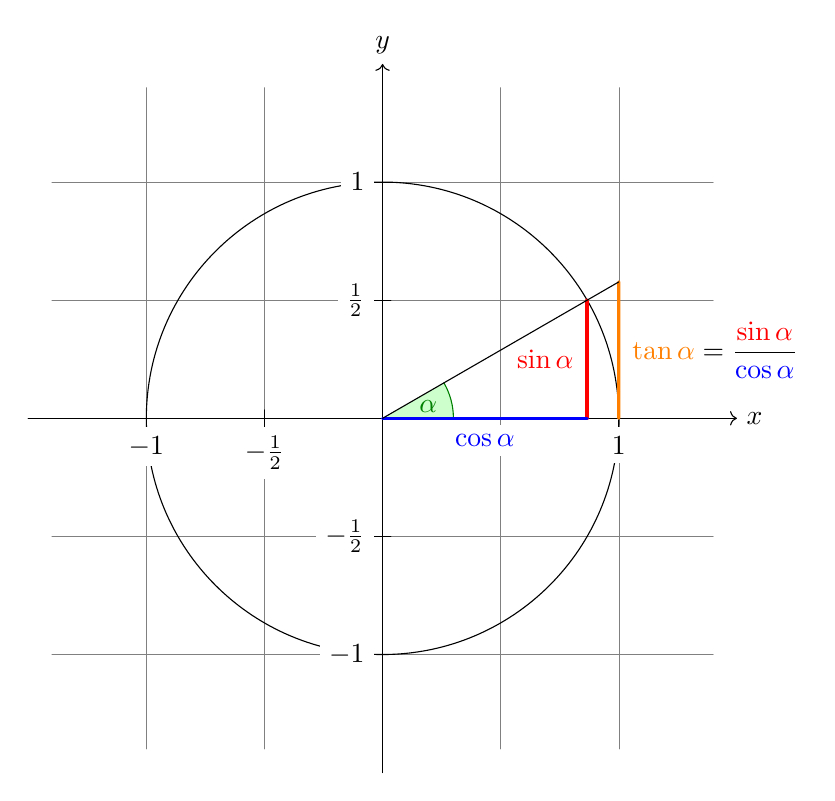
\begin{tikzpicture}[scale=3,line cap=round,
      % Styles
      axes/.style=,
      important line/.style={very thick},
      information text/.style={rounded corners,fill=red!10,inner sep=1ex}]
      % Colors
        \colorlet{anglecolor}{green!50!black}
        \colorlet{sincolor}{red}
        \colorlet{tancolor}{orange!80!black}
        \colorlet{coscolor}{blue}
        % The graphic
        \draw[help lines,step=0.5cm] (-1.4,-1.4) grid (1.4,1.4);
        \draw (0,0) circle [radius=1cm];
        \begin{scope}[axes]
        \draw[->] (-1.5,0) -- (1.5,0) node[right] {$x$} coordinate(x axis);
        \draw[->] (0,-1.5) -- (0,1.5) node[above] {$y$} coordinate(y axis);
        \foreach \x/\xtext in {-1, -.5/-\frac{1}{2}, 1}
        \draw[xshift=\x cm] (0pt,1pt) -- (0pt,-1pt) node[below,fill=white] {$\xtext$};
        \foreach \y/\ytext in {-1, -.5/-\frac{1}{2}, .5/\frac{1}{2}, 1}
        \draw[yshift=\y cm] (1pt,0pt) -- (-1pt,0pt) node[left,fill=white] {$\ytext$};
        \end{scope}
        \filldraw[fill=green!20,draw=anglecolor] (0,0) -- (3mm,0pt)
        arc [start angle=0, end angle=30, radius=3mm];
        \draw (15:2mm) node[anglecolor] {$\alpha$};
        \draw[important line,sincolor]
        (30:1cm) -- node[left=1pt,fill=white] {$\sin \alpha$} (30:1cm |- x axis);
        \draw[important line,coscolor]
        (30:1cm |- x axis) -- node[below=2pt,fill=white] {$\cos \alpha$} (0,0);
        \path [name path=upward line] (1,0) -- (1,1);
        \path [name path=sloped line] (0,0) -- (30:1.5cm);
        \draw [name intersections={of=upward line and sloped line, by=t}]
        [very thick,orange] (1,0) -- node [right=1pt,fill=white]
        {$\displaystyle \tan \alpha \color{black}=
        \frac{{\color{red}\sin \alpha}}{\color{blue}\cos \alpha}$} (t);
        \draw (0,0) -- (t);
      \end{tikzpicture}
    \end{center}
    We know that
    \begin{align*}
      0 \leq \sin(x) \leq x
    \end{align*}
    so as $x\rightarrow 0^+$, $\sin(x) \rightarrow 0$. Similarly, if $x\rightarrow 0^{-}$, then
    \begin{align*}
      \lim_{x\rightarrow 0^{-}}\sin(x) &= \lim_{y\rightarrow 0^{+}} \sin(-y)\\
                                       &= -\lim_{y\rightarrow 0^{+}}\sin(y)\\
                                       &= 0
    \end{align*}
    and
    \begin{align*}
      \lim_{x\rightarrow 0^+} \cos(x) &= \lim_{x\rightarrow 0^{+}} \sqrt{1-\sin^2(x)}\\
                                      &= 1\\
      \lim_{x\rightarrow 0^{-}} \cos(x) &= \lim_{y\rightarrow 0^{+}} \cos(-y)\\
                                        &= \lim_{y\rightarrow 0^{+}}\cos(y)\\
                                        &= 1
    \end{align*}
    \begin{description}
      \item[Claim:] 
        \begin{align*}
          \lim_{x\rightarrow 0}\frac{\sin(x)}{x} &= 1
        \end{align*}
      \item[Proof:] Let $x\rightarrow 0$
        \begin{align*}
          \frac{\sin(x)}{2} \leq \frac{x}{2} &\leq \frac{\tan(x)}{2}\\
          0 \leq \frac{\sin(x)}{x} &\leq 1\\
          \cos(x) &\leq \frac{\sin(x)}{x}\\
          \cos(x) \leq \frac{\sin(x)}{x} &\leq 1\\
          1 \leq \frac{\sin(x)}{x} &\leq 1
        \end{align*}
    \end{description}
  \end{problem}
  \begin{problem}{Strictly Positive Limits}
    Let $D\subseteq \R$, $f:D\rightarrow \R$. Let $c$ be a cluster point of $D$. If $\lim_{x\rightarrow c}f(x) = L > 0$, then $\exists \delta > 0$ and $\exists t > 0$ such that $f(x) > t$ for $x\in \dot{V}_{\delta}(c) \cap D$.
    \tcblower
    Let $\varepsilon = \frac{L}{2}$. Then, $V_{\varepsilon} = (L/2,3L/2)$. So, $\exists \delta > 0$ such that $x\in \dot{V}_{\delta}(c) \Rightarrow f(x) \in V_{\varepsilon}(L)$. Set $t = L/2$.
  \end{problem}
  \begin{problem}{One-Sided Limits}
    Let $f: D\rightarrow \R$.\\
    
    \textbf{Cluster Points:}
    \begin{enumerate}[(i)]
      \item A number $c\in D$ is a right cluster point if $\forall \delta > 0$, $\exists x\in (c,c+\delta) \cap D$
      \item A number $c\in D$ is a left cluster point if $\forall \delta > 0$, $\exists x\in (c-\delta,c) \cap D$.
    \end{enumerate}
    \textbf{Limits:}
    \begin{enumerate}[(i)]
      \item $\displaystyle \lim_{x\rightarrow c^{+}} f(x) = L \xLeftrightarrow{\text{def}}$
        \begin{align*}
          (\forall \varepsilon > 0)(\exists \delta > 0) \ni x\in (c,c+\delta)\cap D \Rightarrow f(x)\in V_{\varepsilon}(L)
        \end{align*}
      \item $\displaystyle \lim_{x\rightarrow c^{-}} f(x) = L \xLeftrightarrow{\text{def}}$
        \begin{align*}
          (\forall \varepsilon > 0)(\exists \delta > 0) \ni x\in (c-\delta,c) \cap D \Rightarrow f(x)\in V_{\varepsilon}(L)
        \end{align*}
    \end{enumerate}
    \textbf{Sequential Definition:}
    \begin{enumerate}[(i)]
      \item Let $c$ be a right cluster point of $D$. $\lim_{x\rightarrow c^{+}} f(x) = L$ if and only if $\forall (x_n)_n \in D\cap (c,\infty)$ with $(x_n)_n \rightarrow c$, we have $(f(x_n))_n \rightarrow L$
      \item Let $c$ be a left cluster point of $D$. $\lim_{x\rightarrow c^{-}} f(x) = L$ if and only if $\forall (x_n)_n \in (-\infty,c) \cap D$ with $(x_n)_n \rightarrow c$, we have $(f(x_n))_n \rightarrow L$.
    \end{enumerate}
  \end{problem}
  \begin{problem}{}
    Let $f:D\rightarrow \R$. Let $c$ be a cluster point of $D$.
    \begin{align*}
      \lim_{x\rightarrow c}f(x) = L \Leftrightarrow \lim_{x\rightarrow c^{-}}f(x) = \lim_{x\rightarrow c^{+}}f(x) = L
    \end{align*}
  \end{problem}
  \begin{problem}{Infinite Limits}
    Let $f: D\rightarrow \R$, and $c$ be a limit point of $D$. Then,
    \begin{align*}
      \lim_{x\rightarrow c}f(x) = \infty \xLeftrightarrow{\text{def}} (\forall M \geq 0)(\exists \delta > 0) \ni x\in \dot{V}_{\delta}(c)\cap D \Rightarrow f(x) \geq M
    \end{align*}
    \vspace{4pt}
    \rule{\textwidth}{0.4pt}
    \vspace{4pt}
    We can also define
    \begin{align*}
      \lim_{x\rightarrow c}f(x) &= -\infty\\
      \lim_{x\rightarrow c^{\pm}}f(x) &= \pm \infty\\
    \end{align*}
  \end{problem}
  \begin{problem}{Infinite Limits, Example}
    \begin{align*}
      \lim_{x\rightarrow 1^{-}}\frac{1}{1-x} &= -\infty
    \end{align*}
    \begin{description}
      \item[Proof:] Let $M\geq 0$ be large. We want $f(x) \geq M$.
        \begin{align*}
          \frac{1}{1-x} &\geq M\\
          1-x &\leq \frac{1}{M}\\
          x &\geq 1-\frac{1}{M}
        \end{align*}
        Set $\delta = \frac{1}{M}$. If $x\in (1-\delta,1)$, then $x\geq 1-\frac{1}{M}$. So, by our work above, $f(x) \geq M$.
    \end{description}
  \end{problem}
  \begin{problem}{Limits at Infinity}
    Let $f: [a,\infty) \rightarrow \R$, $L\in\R$. Then,
    \begin{align*}
      \lim_{x\rightarrow \infty}f(x) = L \xLeftrightarrow{\text{def}} (\forall \varepsilon > 0)(\exists K \geq a) \ni x\geq K \Rightarrow f(x)\in V_{\varepsilon}(L)
    \end{align*}
    \vspace{4pt}
    \rule{\textwidth}{0.4pt}
    \vspace{4pt}
    Similarly, we can define for $f: (-\infty,b] \rightarrow \R$, $L\in \R$
    \begin{align*}
      \lim_{x\rightarrow -\infty} f(x) = L \xLeftrightarrow{\text{def}} (\forall \varepsilon > 0)(\exists K\leq b) \ni x\leq K \Rightarrow f(x)\in V_{\varepsilon}(L)
    \end{align*}
    and for $f: [a,\infty)$ where
    \begin{align*}
      \lim_{x\rightarrow\infty}f(x) = \infty \xLeftrightarrow{\text{def}} (\forall M \geq 0)(\exists K\geq a) \ni x\geq K \Rightarrow f(x) \geq M
    \end{align*}
    and the respective sequential definitions.
  \end{problem}
  \begin{problem}{Limits at Infinity, Example}
    Let $n\in \N$.
    \begin{align*}
      \lim_{x\rightarrow\infty}x^{n} = \infty
    \end{align*}
    \tcblower
    \begin{description}
      \item[Proof:] Let $M$ be large. We want $x^{n} \geq M$. Then, $x\geq M^{1/n}$. Set $K = M^{1/n}$.
    \end{description}
    \vspace{4pt}
    \rule{\textwidth}{0.4pt}
    \vspace{4pt}
    \begin{align*}
      \lim_{x\rightarrow -\infty}x^{n} &= \begin{cases}
        +\infty,&n = 2k\\
        -\infty,& n= 2k+1
      \end{cases}
    \end{align*}
    \vspace{4pt}
    \rule{\textwidth}{0.4pt}
    \vspace{4pt}
    \begin{align*}
      p(x) &= \sum_{k=1}^{n}a_kx^k\\
      \lim_{x\rightarrow\infty}p(x) &= \begin{cases}
        +\infty,&a_n > 0\\
        -\infty&a_n < 0
      \end{cases}
    \end{align*}
    Let $g(x) = x^n$.
    \begin{align*}
      \frac{p(x)}{g(x)} &= a_n + a_{n-1}\frac{1}{x} + \cdots + a_{0}\frac{1}{x^n}\\
      \lim_{x\rightarrow\infty}\frac{p(x)}{g(x)} &= a_n
    \end{align*}
    \begin{problem}{Lemma}
      If $f,g: [a,\infty)\rightarrow \R$, and $g(x) > 0$. If
      \begin{align*}
        \lim_{x\rightarrow \infty}\frac{f(x)}{g(x)} &= L \neq 0
      \end{align*}
      \begin{enumerate}[(1)]
        \item If $L > 0$, then $\lim_{x\rightarrow\infty} f(x) = \infty \Leftrightarrow \lim_{x\rightarrow\infty}g(x) = \infty$
        \item If $L < 0$, then $\lim_{x\rightarrow\infty} f(x)= -\infty \Leftrightarrow \lim_{x\rightarrow\infty}g(x) = +\infty$
      \end{enumerate}
    \end{problem}
    Apply the lemma to $p(x),~x^n$.
  \end{problem}
\end{document}
